\documentclass[twoside,titlepage]{report}

\usepackage{amssymb,amsmath,amsfonts,amsthm,stmaryrd,fancyhdr,graphicx,color}
\usepackage{microtype}
\usepackage{verbatim}
%\usepackage{showkeys} %%% This package will show you your labels
                       %%% and should be commented out for the 
                       %%% final print out.
\usepackage{makeidx} %%% gives us our groovy index
%\usepackage[noDcommand]{kpfonts}

\makeindex

%\usepackage{layout} %%% Use command \layout in document to see margins
%%% Use package mathpazo to get another font

%%% These margins are set for 10 pt font size. 
%%% while some may find them to be too large, they 
%%% are set so that no more than 72 characters will
%%% be on any line.  This will help the readability 
%%% of the document.  If the font size is ever increased
%%% then the margins should be increased a bit too.
\oddsidemargin 62pt
\evensidemargin 62pt
\textwidth 345pt
\headheight 14pt




%%% Header and Footer Options
\renewcommand{\headrulewidth}{0.0pt} %%% this takes out the line 
%%%
%\rhead[]{\textsl{\leftmark}}  %%%
%\rfoot[]{\thepage}            %%% Options for 2 sided documents
%\lhead[\textsl{\rightmark}]{} %%%
%\lfoot[\thepage]{}            %%%
%%%
\lhead[\textsl{\rightmark}]{\textsl{\leftmark}} %%% Options for 1 sided documents
\cfoot[]{}                      %%% With typing on the *left* page
\rhead[]{}                                      %%% 
%%%
\cfoot[\thepage]{\thepage} %%% needed for both types of documents
%%% End Header and Footer Options


%%% This sets how the enumerate command works
\renewcommand{\theenumi}{$(\mathrm{\arabic{enumi}})$}
\renewcommand{\labelenumi}{\theenumi}


%%% This bit of code gives us our nice proof environment.
\renewenvironment{proof}[1][\proofname]{\begin{trivlist}\item[\hskip \labelsep \itshape \bfseries #1{}\hspace{2ex}]}
{\qed\end{trivlist}}
%%%


%%% This next bit of code defines all our theorem environments
\newtheoremstyle{SlantTheorem}{\topsep}{\topsep}%%% space between body and thm
		{\slshape}                      %%% Thm body font
		{}                              %%% Indent amount (empty = no indent)
		{\bfseries\sffamily}            %%% Thm head font
		{}                              %%% Punctuation after thm head
		{3ex}                           %%% Space after thm head
		{\thmname{#1}\thmnumber{ #2}\thmnote{ \bfseries(#3)}}%%% Thm head spec
\theoremstyle{SlantTheorem}
\newtheorem{thm}{Theorem}
\newtheorem*{cor}{Corollary}
\newtheorem*{para}{Paradox}
\newtheorem*{con}{Construction}
\newtheorem*{conj}{Conjecture}
\newtheorem{lem}[thm]{Lemma}
\newtheorem*{war}{WARNING}
\newtheorem*{eg}{Example}

\newtheoremstyle{Definition}
{\topsep}{\topsep}{}{}{\sffamily\bfseries}{}{3ex}{}
\theoremstyle{Definition}
\newtheorem*{dfn}{Definition}

\newtheoremstyle{Exercises}
{\topsep}{\topsep}{}{}{\bfseries}{}{3ex}{}
\theoremstyle{Exercises}
\newtheorem*{ques}{Question}



\newtheoremstyle{problem}{\topsep}{\topsep}%%% space between body and thm
		{}                      %%% Thm body font
		{}                              %%% Indent amount (empty = no indent)
		{\bfseries}            %%% Thm head font
		{)}                    %%% Punctuation after thm head
		{ }                           %%% Space after thm head
		{\thmnumber{#2}\thmnote{ \bfseries (#3)}}%%% Thm head spec
\theoremstyle{problem}
\newtheorem{prob}{}[section]
\renewcommand{\theprob}{\arabic{prob}}


%%% This set of code gives us the unnumbered footnotes
\long\def\symbolfootnote[#1]#2{\begingroup\def\thefootnote{\fnsymbol{footnote}}
\footnote[#1]{#2}\endgroup}


%%% This set of code is all of our user defined commands
\newcommand{\bysame}{\mbox{\rule{3em}{.4pt}}\,}
\newcommand{\N}{\mathbb N}
\newcommand{\Z}{\mathbb Z}
\newcommand{\R}{\mathbb R}
\newcommand{\Q}{\mathbb Q}
\newcommand{\A}{\mathbb A}
\newcommand{\C}{\mathcal C}
\newcommand{\D}{\mathcal D}
\newcommand{\F}{\mathcal F}
\newcommand{\ph}{\varphi}
\newcommand{\ep}{\varepsilon}
\newcommand{\aph}{\alpha}
\newcommand{\QM}{\begin{center}{\huge\textbf{?}}\end{center}}
\renewcommand{\le}{\leqslant}
\renewcommand{\ge}{\geqslant}
\renewcommand{\a}{\wedge}
\renewcommand{\v}{\vee}
\renewcommand{\l}{\ell}
\newcommand{\mat}{\mathsf}
\renewcommand{\vec}{\mathbf}
\renewcommand{\subset}{\subseteq}
\renewcommand{\supset}{\supseteq}
\renewcommand{\emptyset}{\varnothing}
\renewcommand{\qedsymbol}{$\blacksquare$}
\renewcommand{\bibname}{References and Further Reading}
\renewcommand{\abstractname}{Distributing this Document}
\newcommand{\tri}{\triangle}
\newcommand{\minipad}{\vspace{1ex}}
\newcommand{\problems}{\subsection*{Problems for Section~\thesection}\hrule\vspace{1ex}}


\begin{document}

%%%% Front matter


\newpage

\begin{fullwidth}
~\vfill
\thispagestyle{empty}
\setlength{\parindent}{0pt}
\setlength{\parskip}{\baselineskip}
Copyright \copyright~2013 Bart Snapp and Bradford Findell

\vspace{.5cm}

\noindent
This work is licensed under the Creative Commons:
\begin{center}
Attribution-NonCommercial-ShareAlike License 
\end{center}
To view a copy of this license, visit
\[
\texttt{http://creativecommons.org/licenses/by-nc-sa/3.0/}
\]


\vspace{.5cm}
\noindent This document was typeset on \today.
\end{fullwidth}


\chapter*{Preface}
\addcontentsline{toc}{chapter}{Preface}


These notes are designed with future middle grades mathematics
teachers in mind.  While most of the material in these notes would be
accessible to an accelerated middle grades student, it is our hope
that the reader will find these notes both interesting and
challenging.  In some sense we are simply taking the topics from a
middle grades class and pushing ``slightly beyond'' what one might
typically see in schools. In particular, there is an emphasis on the
ability to communicate mathematical ideas.  Three goals of these notes
are:
\begin{itemize}
\item To enrich the reader's understanding of both numbers and algebra. 
From the basic algorithms of arithmetic---all of which have algebraic
underpinnings---to the existence of irrational numbers, we hope to show
the reader that numbers and algebra are deeply connected.
\item To place an emphasis on problem solving. The reader will be exposed 
to problems that ``fight-back.'' Worthy minds such as yours deserve
worthy opponents. Too often mathematics problems fall after a single
``trick.'' Some worthwhile problems take time to solve and cannot be done
in a single sitting.
\item To challenge the common view that mathematics is a body of knowledge 
to be memorized and repeated. The art and science of doing mathematics
is a process of reasoning and personal discovery followed by
justification and explanation. We wish to convey this to the reader,
and sincerely hope that the reader will pass this on to others as
well.
\end{itemize}
In summary---you, the reader, must become a doer of mathematics.  To
this end, many questions are asked in the text that follows. Sometimes
these questions are answered; other times the questions are left for
the reader to ponder. To let the reader know which questions are left
for cogitation, a large question mark is displayed:
\QM
The instructor of the course will address some of these questions. If
a question is not discussed to the reader's satisfaction, then we
encourage the reader to put on a thinking-cap and think, think, think!
If the question is still unresolved, go to the World Wide Web and
search, search, search!

This document is open-source. It is licensed under the Creative
Commons Attribution-NonCommercial-ShareAlike (CC BY-NC-SA)
License. Loosely speaking, this means that this document is available
for free. Anyone can get a free copy of this document 
from the following sites:
\[
\texttt{http://www.math.osu.edu/\~{}snapp/1165/}
\]
\[
\texttt{http://www.math.osu.edu/\~{}findell.2}
\]
Please report corrections, suggestions, gripes, complaints, and
criticisms to Bart Snapp at \texttt{snapp@math.osu.edu} or Brad Findell
at \texttt{findell.2@osu.edu}


\section*{Thanks and Acknowledgments}

This document has a somewhat lengthy history. In the Fall of 2005 and
Spring of 2006, Bart Snapp gave a set of lectures at the University of
Illinois at Urbana-Champaign. His lecture notes were typed and made
available as an open-source textbook. During subsequent semesters, those notes
were revised and modified under the supervision of Alison Ahlgren and
Bart Snapp. Many people have made contributions,
including Tom Cooney, Melissa Dennison, and Jesse Miller. A number of
students also contributed to that document by either typing original
hand-written notes or suggesting problems. They are: Camille Brooks,
Michelle Bruno, Marissa Colatosti, Katie Colby, Anthony `Tino'
Forneris, Amanda Genovise, Melissa Peterson, Nicole Petschenko, Jason
Reczek, Christina Reincke, David Seo, Adam Shalzi, Allice Son, Katie
Strle, and Beth Vaughn.

In 2009, Greg Williams, a Master of Arts in Teaching student at
Coastal Carolina University, worked with Bart Snapp to produce an
early draft of the chapter on isometries.

In the Winter of 2010 and 2011, Bart Snapp gave a new set of lectures
at the Ohio State University. In this course the previous lecture
notes were heavily modified, resulting in a new text \textit{Parallels
in Geometry}.  In 2012 and 2013, Bart Snapp and Brad Findell 
continued revising these notes.  

\makeatletter %% adds space so that the numbers of the toc don't bump
\renewcommand{\l@section}{\@dottedtocline{1}{5em}{5em}}
\renewcommand{\l@subsection}{\@dottedtocline{2}{5em}{5em}}
\renewcommand{\l@subsubsection}{\@dottedtocline{3}{5em}{5em}}
\makeatother


\setcounter{tocdepth}{1}
\tableofcontents

%%%%
\newpage
\pagenumbering{arabic}
\pagestyle{fancy}
%%%%%%%%%%%%%%%%%%%%%%%%%%%%%%%%%%%%%%%%
%%%%%%% Sections to be included %%%%%%%%
%%%%%%%%%%%%%%%%%%%%%%%%%%%%%%%%%%%%%%%%

\chapter{Proof by Picture}

\begin{quote}
A picture is worth a thousand words.

\hfill---Unknown
\end{quote}


\section{Basic Set Theory}

The word \textit{set} has more definitions in the dictionary than any
other word. In our case we'll use the following definition:

\begin{definition}\index{set} 
A \textbf{set} is any collection of elements for which we can always
tell whether an element is in the set or not.
\end{definition}

\begin{question} 
What are some examples of sets? What are some examples of things that
are not sets?
\end{question}
\QM

If we have a set $X$ and the element $x$ is inside of $X$, we write:
\[
x\in X\index{e@$\in$}\index{set theory symbols!in@$\in$}
\]
This notation is said ``$x$ in $X$.'' Pictorially we can imagine this
as:
\[
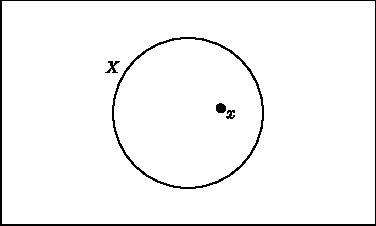
\includegraphics{../graphics/set1.pdf}
\]

\begin{definition} 
A \textbf{subset}\index{subset} $Y$ of a set $X$ is a set $Y$ such
that every element of $Y$ is also an element of $X$. We denote this
by:
\[
Y\subset X\index{set theory symbols!subset@$\subset$}
\] 
\end{definition}

If $Y$ is contained in $X$, we will sometimes loosely say that $X$ is
\textit{bigger} than $Y$.

\begin{question} 
Can you think of a set $X$ and a subset $Y$ where saying $X$ is bigger
than $Y$ is a bit misleading?
\end{question}
\QM

\begin{question} 
How is the meaning of the symbol $\in$ different from the meaning of
the symbol $\subset$?
\end{question}
\QM


\subsection{Union}


\begin{definition}\index{union}\index{u@$\cup$}\index{set theory symbols!union@$\cup$} Given two sets $X$ and $Y$, $X$ \textbf{union} $Y$ is the set of all the elements in $X$ or $Y$. We denote this by $X\cup Y$.  \fixnote{This is inclusive or.}
\end{definition}

Pictorially, we can imagine this as:

\[
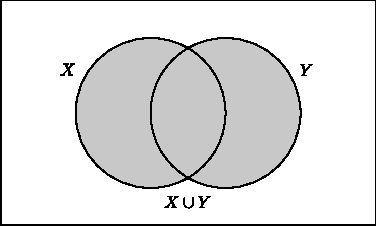
\includegraphics{../graphics/set2.pdf}
\]



\subsection{Intersection}

\begin{definition}\index{intersection}\index{set theory symbols!intersection@$\cap$} Given two sets $X$ and $Y$, 
$X$ \textbf{intersect} $Y$ is the set of all the elements that are simultaneously in $X$ and in $Y$. We denote this by $X\cap Y$. 
\end{definition}

Pictorially, we can imagine this as:
\[
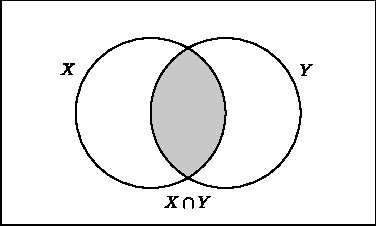
\includegraphics{../graphics/set3.pdf}
\]

\begin{question} Consider the sets $X$ and $Y$ below:
\[
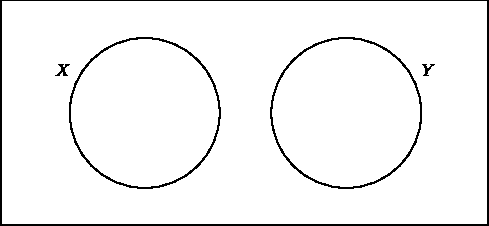
\includegraphics{../graphics/set4.pdf}
\]
What is $X\cap Y$?
\end{question}

I'll take this one: Nothing! We have a special notation for the set with no elements, it is called the \index{empty set}\textbf{empty set}. We denote the empty set by the symbol $\emptyset$.\index{set theory symbols!emptyset@$\emptyset$}  \fixnote{Include subtleties about the empty set.}




\subsection{Complement}

\begin{definition}\index{complement}\index{set theory symbols!complement@$-$} Given two sets $X$ and $Y$, 
$X$ \textbf{complement} $Y$ is the set of all the elements that are in $X$ and are not in $Y$. We denote this by $X-Y$.
\end{definition}

Pictorially, we can imagine this as:
\[
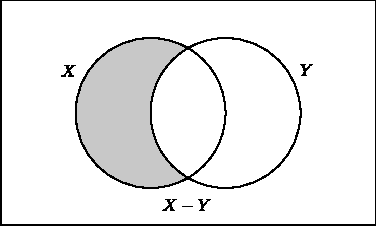
\includegraphics{../graphics/set5.pdf}
\]

\begin{question} Check out the two sets below:
\[
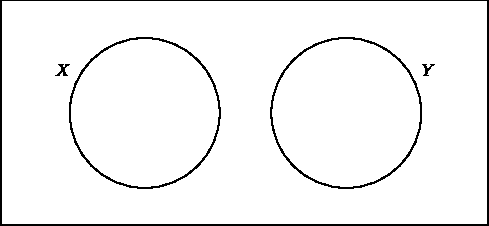
\includegraphics{../graphics/set4.pdf}
\]
What is $X-Y$? What is $Y-X$?
\end{question}
\QM


\subsection{Putting Things Together}

OK, let's try something more complex:

\begin{question} Prove that:
\[
X\cup (Y \cap Z) = (X \cup Y)\cap (X \cup Z)
\]
\end{question}

\begin{proof} 
Look at the left-hand side of the equation first. We can represent the
elements in $Y\cap Z$ with shaded region in the following diagram:
\[
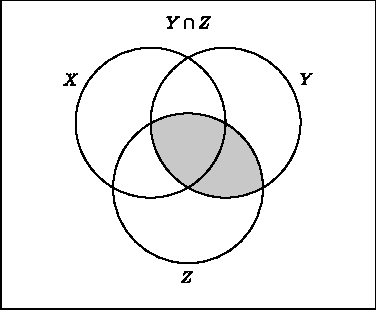
\includegraphics{../graphics/setproof.pdf}
\]
So the union of this region with $X$ is represented the shaded
region in this diagram.
\[
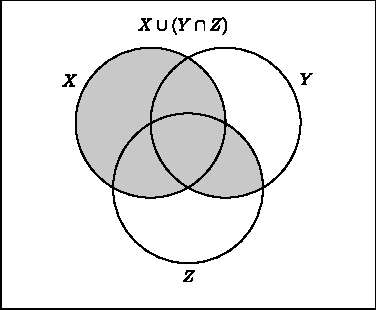
\includegraphics{../graphics/setproof1.pdf}
\]
Now, looking at the right-hand side of the equation, $X\cup Y$ is
represented by this shaded region:
\[
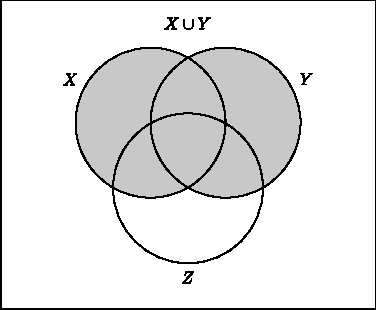
\includegraphics{../graphics/setproof2.pdf}
\]
And $X\cup Z$ is represented by this shaded region:
\[
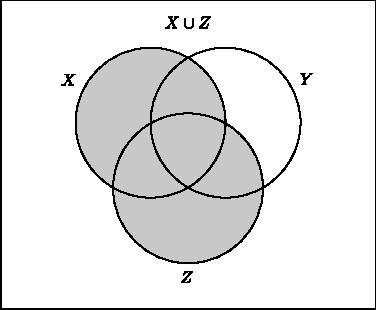
\includegraphics{../graphics/setproof3.pdf}
\]
The region shaded in both of the diagrams, which is the
intersection of $X\cup Y$ and $X\cup Z$, is represented by the shaded
region below.
\[
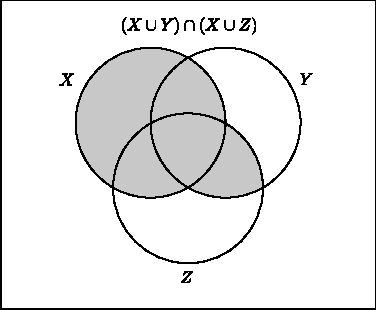
\includegraphics{../graphics/setproof4.pdf}
\]
Comparing the diagrams representing the left-hand and right-hand sides
of the equation, we see that the same regions are shaded, and so we
are done.
\end{proof}

\begin{problems}
\fixnote{Add a problem about exclusive or.}
\begin{enumerate}
\item Given two sets $X$ and $Y$, explain what is meant by $X\cup Y$.
\item Given two sets $X$ and $Y$, explain what is meant by $X\cap Y$.
\item Given two sets $X$ and $Y$, explain what is meant by $X - Y$.
\item Explain the difference between the symbols $\in$ and $\subset$.
\item If we let $X$ be the set of ``right triangles'' and we let $Y$ be the set of ``equilateral triangles'' does the picture below show the relationship between these two sets?
\[
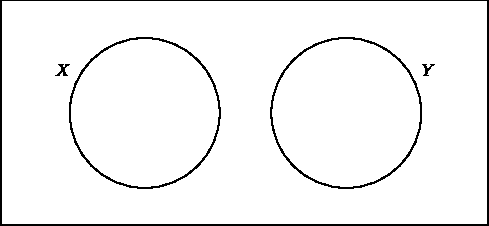
\includegraphics{../graphics/set4.pdf}
\]
Explain your reasoning.
\item If $X = \{1,2,3,4,5\}$ and $Y = \{3,4,5,6\}$ find:
\begin{enumerate}
\item $X\cup Y$
\item $X\cap Y$
\item $X-Y$
\item $Y-X$
\end{enumerate}
In each case explain your reasoning. 
\item Let $n\Z$ represent the integer multiples of $n$. So for example:
\[
3\Z = \{\dots,-12,-9,-6,-3,0,3,6,9,12,\dots\}
\]
Compute the following:
\begin{enumerate}
\item $3\Z\cap 4\Z$
\item $2\Z\cap 5\Z$
\item $3\Z\cap 6\Z$
\item $4\Z\cap 6\Z$
\item $4\Z\cap 10\Z$
\end{enumerate}
In each case explain your reasoning. 
\item Make a general rule for intersecting sets of the form $n\Z$ and
  $m\Z$. Explain why your rule works.
\item Prove that:
\[
X = (X\cap Y) \cup (X-Y)
\]
\item Prove that:
\[
X-(X-Y) = (X\cap Y)
\]
\item Prove that:
\[
X \cup (Y-X) = (X\cup Y)
\]
\item Prove that:
\[
X \cap (Y-X) = \emptyset
\]
\item Prove that:
\[
(X-Y)\cup (Y-X) = (X\cup Y)-(X\cap Y)
\]
\item Prove that:
\[
X\cup (Y \cap Z) = (X \cup Y)\cap (X \cup Z)
\]
\item Prove that:
\[
X\cap (Y \cup Z) = (X \cap Y)\cup (X \cap Z)
\]
\item Prove that:
\[
X - (Y \cap Z) = (X -Y)\cup (X - Z)
\]
\item Prove that:
\[
X - (Y \cup Z) = (X -Y)\cap (X -Z)
\]
\item If $X\cup Y = X$, what can we say about the relationship between the sets $X$ and $Y$? Explain your reasoning.
\item If $X\cup Y = Y$, what can we say about the relationship between the sets $X$ and $Y$? Explain your reasoning.
\item If $X\cap Y = X$, what can we say about the relationship between the sets $X$ and $Y$? Explain your reasoning.
\item If $X\cap Y = Y$, what can we say about the relationship between the sets $X$ and $Y$? Explain your reasoning.
\item If $X-Y =\emptyset$, what can we say about the relationship between the sets $X$ and $Y$? Explain your reasoning.
\item If $Y-X =\emptyset$, what can we say about the relationship between the sets $X$ and $Y$? Explain your reasoning.
\end{enumerate}
\end{problems}


\newpage



\section{Tessellations}

Go to the internet and look up M.C.\ Escher.\index{Escher, M.C.} He
was an artist. Look at some of his work. When you do your search be
sure to include the word ``tessellation'' OK? Back already? Very
good. Sometimes Escher worked with tessellations. What's a
tessellation? I'm glad you asked:

\begin{definition}\index{tessellation} A \textbf{tessellation} is a pattern of 
polygons fitted together to cover the entire plane without
overlapping.  
\end{definition}
While it is impossible to actually cover the entire plane with shapes,
if we give you enough of a tessellation, you should be able to continue
it's pattern indefinitely.  Here are pieces of tessellations:
\[
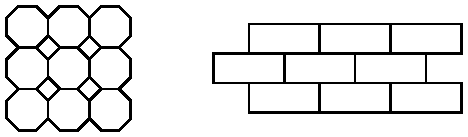
\includegraphics{../graphics/semiRegTess.pdf}
\]
On the left we have a tessellation of a square and an octagon. On the
right we have a ``brick-like'' tessellation.

\begin{definition}\index{tessellation!regular}\index{regular!tessellation}
A tessellation is called a \textbf{regular tessellation} if it is
composed of copies of a single regular polygon and these polygons meet
vertex to vertex.\index{regular!polygon}
\end{definition}


\begin{example} Here are some examples of regular tessellations:
\[
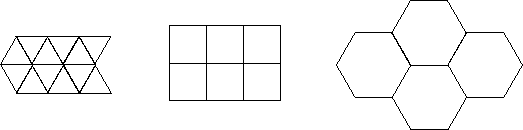
\includegraphics{../graphics/regtess.pdf}
\]
\end{example}

Johannes Kepler\index{Kepler, Johannes}, who lived from 1571--1630,
was one of the first people to study tessellations. He certainly knew
the next theorem:

\begin{theorem} There are only $3$ regular tessellations.
\end{theorem}

\begin{question} Why is the theorem above true?
\end{question}
\QM

Since one can prove that there are only three regular tessellations,
and we have shown three above, then that is all of them. On the other
hand there are lots of nonregular tessellations. Here are two
different ways to tessellate the plane with a
triangle:\index{tessellation!triangles}
\[
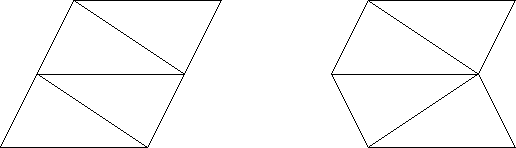
\includegraphics{../graphics/triangletess.pdf}
\]
Here is a way that you can tessellate the plane with any old
quadrilateral:
\[\index{tessellation!any quadrilateral}\index{quadrilateral!tessellation of}
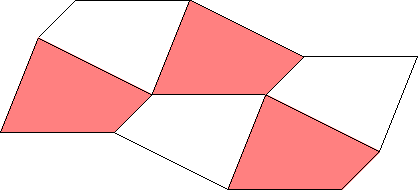
\includegraphics{../graphics/quadtess.pdf}
\]

\subsection{Tessellations and Art}

How does one make art with tessellations? To start, a little
decoration goes a long way. Check this out: Decorate two squares as
such:
\[

\includegraphics{../graphics/lightningsquares.pdf}
\]
Tessellate them randomly in the plane to get this lightning-like picture:
\[

\includegraphics{../graphics/lightningtess.pdf}
\]
\begin{question} 
What sort of picture do you get if you tessellate these decorated
squares randomly in a plane?
\[
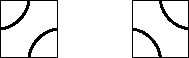
\includegraphics{../graphics/watersquares.pdf}
\]
\end{question}
\QM

Another way to go is to start with your favorite tessellation:
\[
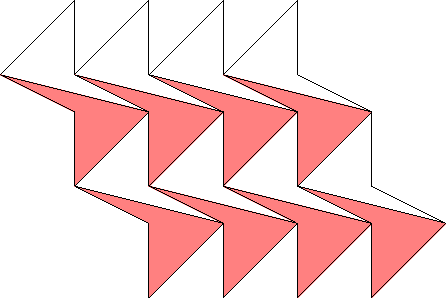
\includegraphics{../graphics/nonconvextess.pdf}
\]
Then you modify it a bunch to get something different:
\[
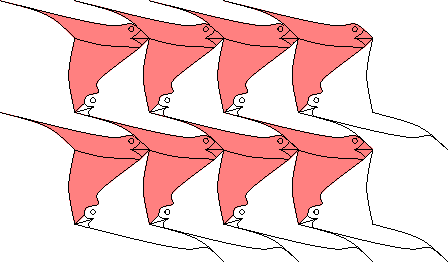
\includegraphics{../graphics/birdstess.pdf}
\]

\begin{question} What kind of art can you make with tessellations?
\end{question}
\QM


I'm not a very good artist, but I am a mathematician. So let's use a
tessellation to give a proof! Let me ask you something:

\begin{question} What is the most famous theorem in mathematics? 
\end{question}
Probably the Pythagorean Theorem comes to mind. Let's recall the statement of the Pythagorean Theorem:

\begin{theorem}[Pythagorean Theorem]\index{Pythagorean Theorem} Given a right triangle, the sum of the squares of the 
lengths of the two legs equals the square of the length of 
the hypotenuse.  Symbolically, if $a$ and $b$ represent the 
lengths of the legs and $c$ is the length of the hypotenuse, 
\[
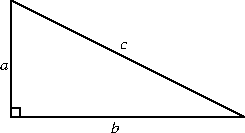
\includegraphics{../graphics/pbppyth.pdf}
\]
then 
\[
a^2 + b^2 = c^2.
\]
\end{theorem}


Let's give a proof! Check out this tessellation involving $2$ squares:
\[
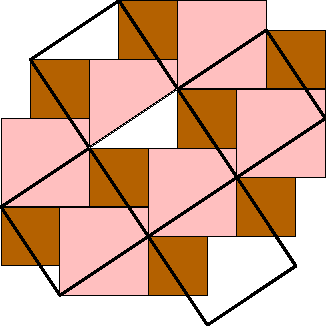
\includegraphics{../graphics/pbppyth2.pdf}
\]
\begin{question} How does the picture above ``prove'' the Pythagorean Theorem?
\end{question}
\begin{proof}[Solution]  
The white triangle is our right triangle. The area of the middle
overlaid square is $c^2$, the area of the small dark squares is $a^2$,
and the area of the medium lighter square is $b^2$. Now label all the
``parts'' of the large overlaid square:
\[
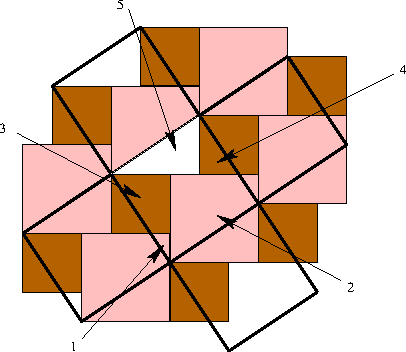
\includegraphics{../graphics/pbppyth2a.pdf}
\]
From the picture we see that
\begin{align*}
a^2 &= \{\text{3 and 4}\}\\
b^2 &= \{\text{1, 2, and 5}\}\\
c^2 &= \{\text{1, 2, 3, 4, and 5}\}
\end{align*}
Hence
\[
c^2 = a^2 + b^2
\]
Since we can always put two squares together in this pattern, this
proof will work for any right triangle.
\end{proof}

\begin{question} Can you use the above tessellation to give a dissection proof of the Pythagorean Theorem?
\end{question}
\QM



\begin{problems}

\begin{enumerate}
\item Show two different ways of tessellating the plane with a given scalene triangle. Label your picture as necessary.
\item Show how to tessellate the plane with a given quadrilateral. Label your picture.
\item Show how to tessellate the plane with a nonregular hexagon. Label your picture.
\item Give an example of a polygon with $9$ sides that tessellates the plane.
\item Give examples of polygons that tessellate and polygons that do
  not tessellate.
\item Give an example of a triangle that tessellates the plane where
  both $4$ and $8$ angles fit around each vertex.
\item True or False: Explain your conclusions.
\begin{enumerate}
\item There are exactly 5 regular tessellations.
\item Any quadrilateral tessellates the plane.
\item Any triangle will tessellate the plane.
\item If a triangle is used to tessellate the plane, then it is always
  the case that exactly $6$ angles will fit around each vertex.
\item If a polygon has more than 6 sides, then it cannot tessellate the plane.
\end{enumerate}
\item Given a regular tessellation, what is the sum of the angles
  around a given vertex?
\item Given that the regular octagon has $135$ degree angles, explain
  why you cannot give a regular tessellation of the plane with a
  regular octagon.
\item \label{tesstable} Fill in the following table:
\begin{center}
\begin{tabular}{|c || c| c| c|}\hline
 Regular & Does it      &  Measure & If it tessellates, how  \\
 $n$-gon & tessellate?  &  of an angle &  many surround each vertex?  \\
\hline\hline
$3$-gon &  &  &  \\ \hline
$4$-gon &  &  &  \\ \hline
$5$-gon &  &  &  \\ \hline
$6$-gon &  &  &  \\ \hline
$7$-gon &  &  &  \\ \hline
$8$-gon &  &  &  \\ \hline
$9$-gon &  &  &  \\ \hline
$10$-gon &  &  &  \\ \hline
\end{tabular}
\end{center}
Hint: A regular $n$-gon has interior angles of $180(n-2)/n$ degrees. 
\begin{enumerate}
\item What do the shapes that tessellate have in common?
\item Make a graph with the number of sides of an $n$-gon on the
  horizontal axis and the measure of a single angle on the vertical
  axis. Briefly describe the relationship between the number of sides
  of a regular $n$-gon and the measure of one of its angles.
\item What regular polygons \textit{could} a bee use for building
  hives? Give some reasons that bees seem to use hexagons.\index{bees}
\end{enumerate}
\item Considering that the regular $n$-gon has interior angles of
  $180(n-2)/n$ degrees, and Problem \ref{tesstable} above, prove that
  there are only 3 regular tessellations of the plane.
\item Explain how the following picture ``proves'' the Pythagorean
  Theorem.
\[
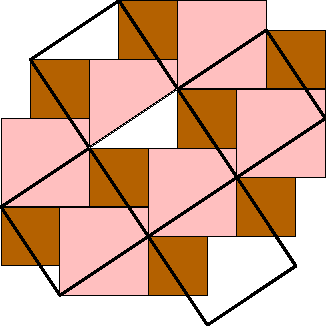
\includegraphics{../graphics/pbppyth2.pdf}
\]
\end{enumerate}
\end{problems}


\newpage



\section{Proof by Picture}
\marginnote{Most of the \textit{pictures} from this section are adapted from the wonderful source books: \cite{nelsen} and \cite{nelsen1}.}  

Pictures generally do not constitute a proof on their own. However, a
good picture can show insight and communicate concepts better than
words alone. In this section we will show you pictures giving the idea
of a proof and then ask you to supply the words to finish off the
argument. 


\subsection{Proofs Involving Right Triangles}

Let's start with something easy:

\begin{question} Explain how the following picture ``proves'' that
  the area of a right triangle is half the base times the height.
\[
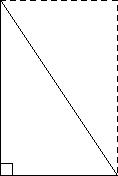
\includegraphics{../graphics/pbpAreaRight.pdf}
\]
\end{question}
\QM 

That wasn't so bad was it? Now for a game of \textit{whose-who}:

\begin{question} What is the most famous theorem in mathematics? 
\end{question}
Probably the Pythagorean Theorem comes to mind. Let's recall the statement of the Pythagorean Theorem:

\begin{theorem}[Pythagorean Theorem]\index{Pythagorean Theorem} Given a right triangle, the sum of the squares of the 
lengths of the two legs equals the square of the length of 
the hypotenuse.  Symbolically, if $a$ and $b$ represent the 
lengths of the legs and $c$ is the length of the hypotenuse, 
\[
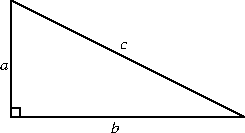
\includegraphics{../graphics/pbppyth.pdf}
\]
then 
\[
a^2 + b^2 = c^2.
\]
\end{theorem}
\begin{question} What is the converse to the Pythagorean Theorem? Is it true? How do you prove it?
\end{question}
\QM

While everyone may know the Pythagorean Theorem, not as many know how to prove it. Euclid's proof goes kind of like this: 

Consider the following picture:
\[
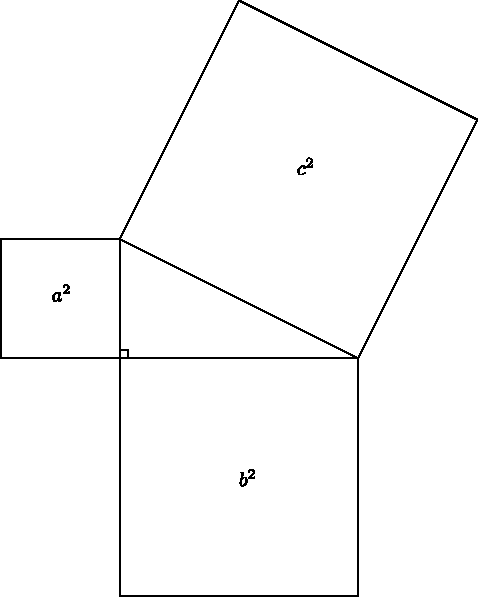
\includegraphics[scale=0.8]{../graphics/pbppythsqr.pdf}
\]
Now, cut up the squares $a^2$ and $b^2$ in such a way that they fit into $c^2$ perfectly. When you give a proof that involves cutting up the shapes and putting them back together, it is called a \textbf{dissection proof}.\index{dissection proof} The trick to ensure that this is actually a proof is in making sure
that your dissection will work no matter what right triangle you are
given. Does it sound complicated? Well it can be. 


Is there an easier proof?  Sure, look at:
\[
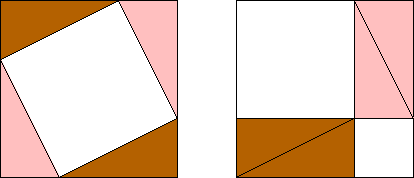
\includegraphics{../graphics/pbppyth1.pdf}
\]
\begin{question} How does the picture above ``prove'' the Pythagorean Theorem?
\end{question}


\begin{proof}[Solution] Both of the large squares above are the same size. Moreover both the unshaded regions above must have the same area. The large white square on the left has an area of $c^2$ and the two white squares on the right have a combined area of $a^2 + b^2$. Thus we see that:
\[
c^2 = a^2 + b^2
\]
\end{proof}


Now a paradox:

\begin{paradox}\index{paradox!triangle dissection} What is wrong with this picture?
\[
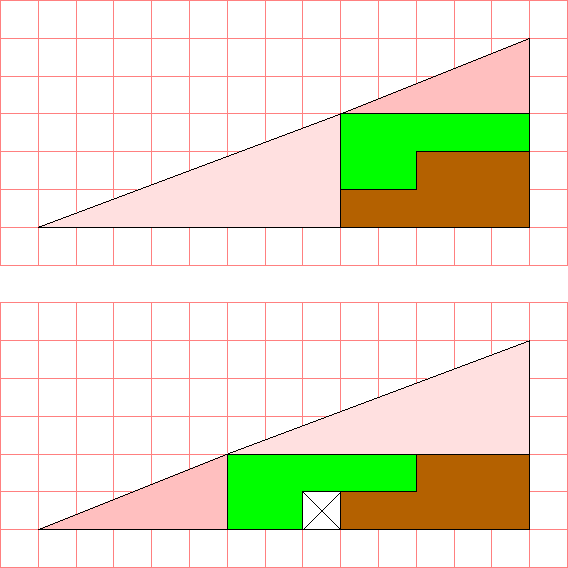
\includegraphics[scale=0.8]{../graphics/triparadox.pdf}
\]
\end{paradox}

\begin{question} 
How does this happen?   
% (See CITATION ERROR % \cite{gardner2} 
% Chapter 8, for a wonderful discussion of puzzling pictures like this one.)
\end{question}
\QM

\subsection{Proofs Involving Boxy Things}

Consider the problem of \textit{Doubling the Cube}.\index{doubling the cube} If a mathematician asks us to double a cube, he or she is asking us to double the \textbf{volume} of a given cube. One may be tempted to merely double each side, but this doesn't double the volume! 

\begin{question} Why doesn't doubling each side of the cube double the volume of the cube? 
\end{question}
\QM

Well, let's answer an easier question first. How do you double the area of a square? Does taking each side and doubling it work? 
\[
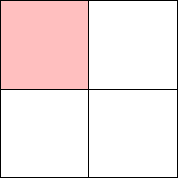
\includegraphics{../graphics/pbpsquare.pdf}
\]
No!  You now have four times the area. So you \textbf{cannot} double the area of a square merely by doubling each side.
What about for the cube? Can you double the volume of a cube merely by doubling the length of every side? Check this out:
\[
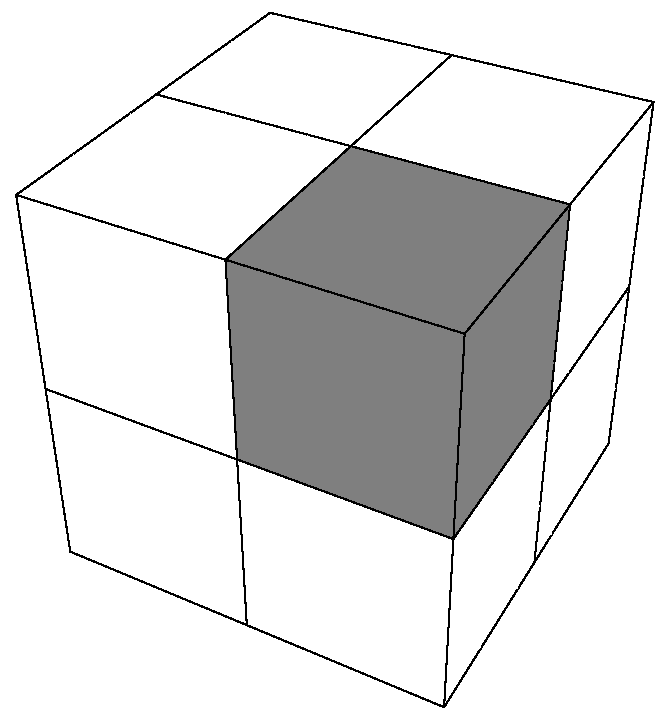
\includegraphics[scale=.4]{../graphics/119VolumeCube.pdf}
\]
Ah, so the answer is again no. If you double each side of a cube you have $8$ times the volume.

\begin{question}
What happens to the area of a square if you multiply the sides by an
arbitrary integer? What about the volume of a cube? Can you explain
what is happening here?
\end{question} 
\QM



\subsection{Proofs Involving Infinite Sums}

As is our style, we will start off with a question:

\begin{question} Can you add up an infinite number of terms and still get a 
finite number?
\end{question}


Consider $1/3$.  Actually, consider the decimal notation for $1/3$:
\[
\frac{1}{3} = .333333333333333333333333333333\dots
\]
But this is merely the sum:
\[
.3 + .03 + .003 + .0003 + .00003 + .000003 + \cdots
\]
It stays less than $1$ because the terms get so small so 
quickly.  Are there other infinite sums of this sort?  You 
bet! Check out this picture:
\[
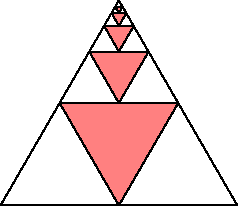
\includegraphics{../graphics/pbptriangle.pdf}
\]
\begin{question} Explain how the picture above ``proves'' that:
\[
\frac{1}{4} + \left(\frac{1}{4}\right)^2 +  \left(\frac{1}{4}\right)^3 +  \left(\frac{1}{4}\right)^4 +  \left(\frac{1}{4}\right)^5 + \cdots = \frac{1}{3}
\]
\end{question}

\begin{proof}[Solution] Let's take it in steps.  If the big triangle has area 
$1$, the area of the shaded region below is $1/4$. 
\[
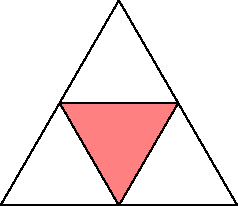
\includegraphics{../graphics/pbptriangle1.pdf}
\]
We also see that the area of the shaded region below 
\[
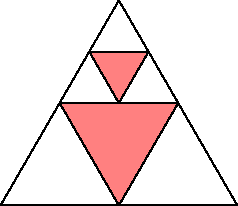
\includegraphics{../graphics/pbptriangle2.pdf}
\]
is:
\[
\frac{1}{4} + \left(\frac{1}{4}\right)^2
\]
Continuing on in this fashion we see that the area of all the shaded regions is:
\[
\frac{1}{4} + \left(\frac{1}{4}\right)^2 +  \left(\frac{1}{4}\right)^3 +  \left(\frac{1}{4}\right)^4 +  \left(\frac{1}{4}\right)^5 + \cdots
\]
But look, the unshaded triangles have twice as much area as 
the shaded triangle.  Thus the shaded triangles must have an
area of $1/3$.
\end{proof}



\subsection{Thinking Outside the Box}


A \textit{calisson}\index{calisson} is a French candy that sort of looks like two equilateral triangles stuck together. They usually come in a hexagon-shaped box. 

\begin{question} How do the calissons fit into their hexagon-shaped box?
\end{question}

If you start to put the calissons into a box, you quickly see that they can be placed in there with exactly three different orientations:
\[
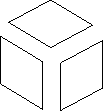
\includegraphics{../graphics/pbporicas.pdf}
\]
\begin{theorem}\label{T:cal} In any packing, the number of calissons with a given orientation is exactly one-third the total number of calissons in the box.
\end{theorem}

Look at this picture:
\[
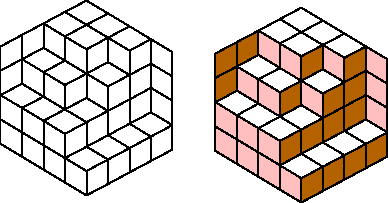
\includegraphics{../graphics/pbpcas.pdf}
\]

\begin{question} How does the picture above ``prove'' Theorem~\ref{T:cal}? Hint: Think outside the box!
\end{question}
\QM




\begin{problems}
\begin{enumerate}
\item Explain the rule
\[
\text{even} + \text{even} = \text{even}
\]
in two different ways. First give an explanation based on
pictures. Second give an explanation based on algebra. 
\item Explain the rule
\[
\text{odd} + \text{even} = \text{odd}
\]
in two different ways. First give an explanation based on
pictures. Second give an explanation based on algebra.
\item Explain the rule
\[
\text{odd} + \text{odd} = \text{even}
\]
in two different ways. First give an explanation based on
pictures. Second give an explanation based on algebra.
\item Explain the rule
\[
\text{even} \cdot \text{even} = \text{even}
\]
in two different ways. First give an explanation based on
pictures. Second give an explanation based on algebra.
\item Explain the rule
\[
\text{odd} \cdot \text{odd} = \text{odd}
\]
in two different ways. First give an explanation based on
pictures. Second give an explanation based on algebra.
\item Explain the rule
\[
\text{odd} \cdot \text{even} = \text{even}
\]
in two different ways. First give an explanation based on
pictures. Second give an explanation based on algebra.
\item\label{P:RTA} Explain how the following picture ``proves'' that
  the area of a right triangle is half the base times the height.
\[
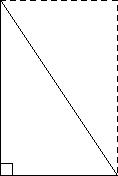
\includegraphics{../graphics/pbpAreaRight.pdf}
\]

\item Suppose you know that the area of a \textbf{right} triangle is
  half the base times the height. Explain how the following picture
  ``proves'' that the area of \textbf{every} triangle is half the base times the
  height.
\[
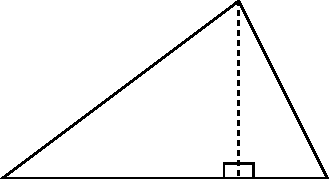
\includegraphics{../graphics/pbpDisTri.pdf}
\]
Now suppose that a student, say \textit{Geometry Giorgio} attempts to
solve a similar problem. Again knowing that the area of a right
triangle is half the base times the height, he draws the following
picture:
\[
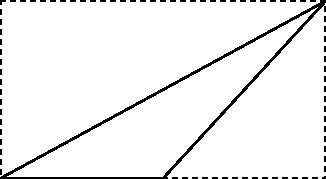
\includegraphics{../graphics/pbpDisTriGio.pdf}
\]
\textit{Geometry Giorgio} states that the diagonal line cuts the
rectangle in half, and thus the area of the triangle is half the base
times the height. Is this correct reasoning? If so, give a complete
explanation. If not, give correct reasoning based on \textit{Geometry
  Giorgio}'s picture.


\item Suppose you know that the area of a \textbf{right} triangle is
  half the base times the height. Explain how the following picture
  ``proves'' that the area of any triangle is half the base times the
  height. Note, this way of thinking is the basis for Cavalieri's
  Principle.\index{Cavalieri's Principle}
\[
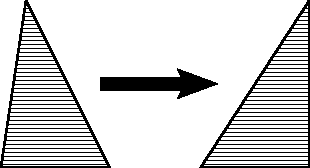
\includegraphics{../graphics/pbpShearTri.pdf}
\]
\item Explain how the following picture ``proves'' that the area of
  any parallelogram is base times height. Note, this way of thinking
  is the basis for Cavalieri's Principle.\index{Cavalieri's Principle}
\[
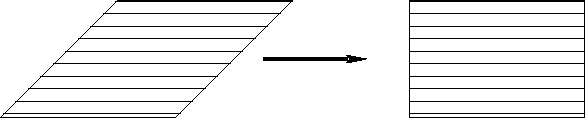
\includegraphics{../graphics/pbpShearPara.pdf}
\]

\item Explain how to use a picture to ``prove'' that a triangle of a
  given area could have an arbitrarily large perimeter.

\item Give two explanations of how the following picture ``proves''
  the Pythagorean Theorem, one using algebra and one without algebra. 
\[
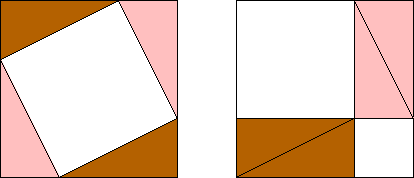
\includegraphics{../graphics/pbppyth1.pdf}
\]
\item Give two explanations of how the following picture ``proves''
  the Pythagorean Theorem, one using algebra and one without algebra. 
\[
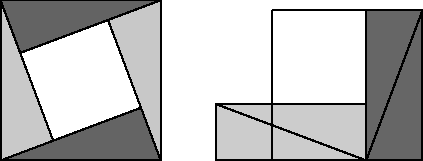
\includegraphics{../graphics/pbppyth3.pdf}
\]
\item Explain how the following picture ``proves'' the Pythagorean Theorem.
\[
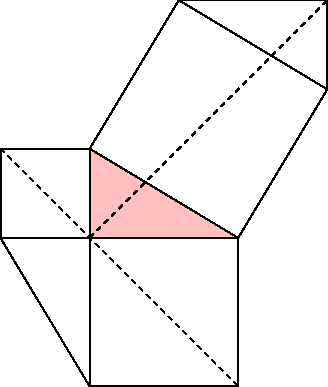
\includegraphics{../graphics/pbpdavinci.pdf}
\]
Note: This proof is due to Leonardo da Vinci.
%\item Explain how the following picture ``proves'' the Pythagorean Theorem.
%\[
%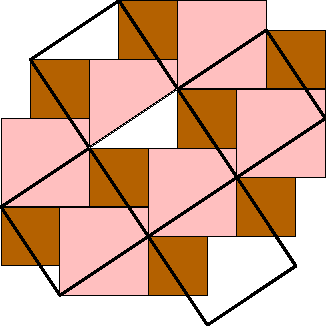
\includegraphics{../graphics/pbppyth2.pdf}
%\]
%\item Use the following tessellation to give a dissection proof of the Pythagorean Theorem.
%\[
%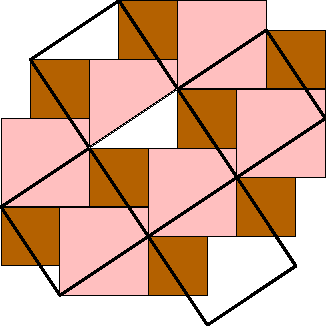
\includegraphics{../graphics/pbppyth2.pdf}
%\]
%\item Explain how the following picture ``proves'' the Pythagorean Theorem.
%\[
%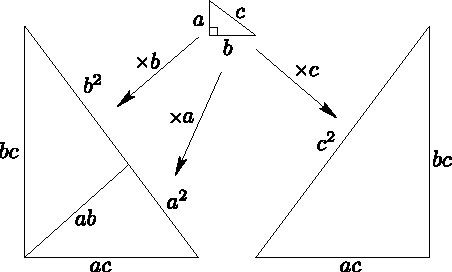
\includegraphics{../graphics/pbpdilation.pdf}
%\]
\item\label{P:pbptrap} Recall that a trapezoid is a quadrilateral with two parallel sides. Consider the following picture:
\[
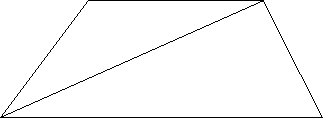
\includegraphics{../graphics/trap.pdf}
\]
How does the above picture prove that the area of a trapezoid is
\[
\mathrm{area}= \frac{h(b_1 + b_2)}{2},
\]
where $h$ is the height of the trapezoid and $b_1$, $b_2$, are the lengths of the parallel sides?
\item Explain how the following picture ``proves'' the Pythagorean Theorem.
\[
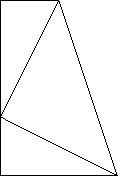
\includegraphics{../graphics/pbptrap.pdf}
\]
Note: This proof is due to James A.\ Garfield, the 20th President of the United States.
\item Look at Problem~\ref{P:pbptrap}. Can you use a similar picture
  to prove that the area of a parallelogram
\[
\includegraphics{../graphics/para.pdf}
\]
is the length of the base times the height?
\item Explain how the following picture ``proves'' that the area of a
  parallelogram is base times height.
\[
\includegraphics{../graphics/para3.pdf}
\]
Now suppose that a student, say \textit{Geometry Giorgio} attempts to
solve a similar problem. In an attempt to prove the formula for the
area of a parallelogram, \textit{Geometry Giorgio} draws the following
picture:
\[
\includegraphics{../graphics/paragiorgio.pdf}
\]
At this point \textit{Geometry Giorgio} says that he has proved the
formula for area of a parallelogram. What do you think of his picture?
Give a complete argument based on his picture.

\item Which of the above ``proofs'' for the formula for the area of a
  parallelogram is your favorite? Explain why.

\item Explain how the following picture ``proves'' that the area of a
  quadrilateral is equal to half of the area of the parallelogram
  whose sides are parallel to and equal in length to the diagonals of
  the original quadrilateral.
\[
\includegraphics[scale=.7]{../graphics/pbpquadarea.pdf}
\]

\item Explain how the following picture ``proves'' that if a
  quadrilateral has two opposite angles that are equal, then the
  bisectors of the other two angles are parallel or on top of each
  other.
\[
\includegraphics[scale=.7]{../graphics/119hw5_2.pdf}
\]



\break

\item\label{P:Tparadox1} Why might someone find the following picture
  disturbing? How would you assure them that actually everything is
  good and well in the geometrical world?
\[
\includegraphics[scale=.8]{../graphics/triparadox.pdf}
\]



\item\label{P:Tparadox2} Why might someone find the following picture
  disturbing? How would you assure them that actually everything is
  good and well in the geometrical world?
\[
\includegraphics[scale=.8]{../graphics/triparadox2.pdf}
\]


\item How could you explain to someone that doubling the lengths of each side of a cube does not double the volume of the cube?

\item\label{P:sq1}  Explain how the following picture ``proves'' that:
\[
\frac{1}{2} + \left(\frac{1}{2}\right)^2 +  \left(\frac{1}{2}\right)^3 +  \left(\frac{1}{2}\right)^4 +  \left(\frac{1}{2}\right)^5 + \cdots = 1
\]
\[
\includegraphics{../graphics/pbpsqgeo.pdf}
\]
\item\label{P:sq2}  Explain how the following picture ``proves'' that if $0 < r < 1$:
\[
r + r(1-r) + r(1-r)^2 + r(1-r)^3 + \cdots = 1
\]
\[
\includegraphics{../graphics/pbpgengeo.pdf}
\]
\item\label{P:tri1} Explain how the following picture ``proves'' that:
\[
\frac{1}{4} + \left(\frac{1}{4}\right)^2 +  \left(\frac{1}{4}\right)^3 +  \left(\frac{1}{4}\right)^4 +  \left(\frac{1}{4}\right)^5 + \cdots = \frac{1}{3}
\]
\[
\includegraphics{../graphics/pbptriangle.pdf}
\]
\item Considering Problem~\ref{P:sq1}, Problem~\ref{P:sq2}, and
  Problem~\ref{P:tri1} can you give a new picture ``proving'' that: 
\[
\frac{1}{4} + \left(\frac{1}{4}\right)^2 +  \left(\frac{1}{4}\right)^3 +  \left(\frac{1}{4}\right)^4 +  \left(\frac{1}{4}\right)^5 + \cdots = \frac{1}{3}
\]
Carefully explain the connection between your picture and the
mathematical expression above.

\item Explain how the following picture ``proves'' that  in any packing, the number of calissons with a given orientation is exactly one-third the total number of calissons in the box.
\[
\includegraphics{../graphics/pbpcas.pdf}
\]
\end{enumerate}
\end{problems}


\chapter{Compass and Straightedge Constructions}
\begin{quote} 
\begin{tabular}{rl}
\textit{Mephistopheles:} & I must say there is an obstacle \\
                         & That prevents my leaving:\\
                         & It's the pentagram on your threshold.\\
\textit{Faust:}          & The pentagram impedes you? \\
                         & Tell me then, you son of hell,\\
                         & If this stops you, how did you come in?\\
\textit{Mephistopheles:} & Observe! The lines are poorly drawn;\\
                         & That one, the outer angle, \\
                         & Is open, the lines don't meet.
\end{tabular}

\hfill---G\"othe, \textit{Faust} act I, scene III
\end{quote}

\section{Constructions}

About a century before the time of \index{Euclid}Euclid,
\index{Plato}Plato---a student of \index{Socrates}Socrates---declared
that the compass and straightedge should be the only tools of the
geometer. Why would he do such a thing? For one thing, both the the
compass and straightedge are fairly simple instruments. One draws
circles, the other draws lines---what else could possibly be needed to
study geometry? Moreover, rulers and protractors are far more complex
in comparison and people back then couldn't just walk to the campus
bookstore and buy whatever they wanted. However, there are other
reasons:
\begin{enumerate}        
\item Compass and straightedge constructions are \textbf{independent
  of units}.
\item Compass and straightedge constructions are \textbf{theoretically
  correct}.
\item Combined, the compass and straightedge seem like
  \textbf{powerful tools}.
\end{enumerate}



\paragraph{Compass and straightedge constructions are \textbf{independent of units}.} 
Whether you are working in centimeters or miles, compass and
straightedge constructions work just as well. By not being locked to
set of units, the constructions given by a compass and straightedge
have certain generality that is appreciated even today.


\paragraph{Compass and straightedge constructions are \textbf{theoretically correct}.} 
In mathematics, a correct method to solve a problem is more valuable
than a correct solution. In this sense, the compass and straightedge
are ideal tools for the mathematician. Easy enough to use that the
rough drawings that they produce can be somewhat relied upon, yet
simple enough that the tools themselves can be described
theoretically. Hence it is usually not too difficult to connect a
given construction to a formal proof showing that the construction is
correct.


\paragraph{Combined, the compass and straightedge seem like \textbf{powerful tools}.} 
No tool is useful unless it can solve a lot of problems. Without a
doubt, the compass and straightedge combined form a powerful
tool. Using a compass and straightedge, we are able to solve many
problems exactly. Of the problems that we cannot solve exactly, we can
always produce an approximate solution.





\index{constructions|see{compass and straightedge \textit{or}
    origami}} We'll start by giving the rules of compass and
straightedge constructions:

\subsubsection*{Rules for Compass and Straightedge Constructions}
\begin{enumerate}
\item You may only use a compass and straightedge.
\item You must have two points to draw a line.
\item You must have a point and a line segment to draw a circle. The
  point is the center and the line segment gives the radius.
\item Points can only be placed in two ways:
\begin{enumerate}
\item As the intersection of lines and/or circles.
\item As a \textbf{free point}\index{free point}, meaning the location
  of the point is not important for the final outcome of the
  construction.
\end{enumerate}
\end{enumerate}

Our first construction is also Euclid's first construction:

\begin{con}[Equilateral Triangle]\index{compass and straightedge!equilateral triangle} We wish to construct an equilateral triangle given the length of one 
side.
\begin{enumerate} 
\item Open your compass to the width of the line segment.
\item Draw two circles, one with the center being each end point 
of the line segment.
\item The two circles intersect at two points.  Choose one and 
connect it to both of the line segment's endpoints.
\end{enumerate}
\[
\includegraphics{../graphics/eqtri.pdf}
\]
\end{con}

Euclid's second construction will also be our second construction:

\begin{con}[Transferring a Segment]\index{compass and straightedge!transferring a segment}
Given a segment, we wish to move it so that it starts on a given
point, on a given line.
\begin{enumerate}        
\item Draw a line through the point in question.
\item Open your compass to the length of the line segment and draw a circle with the given point as its center.
\item The line segment consisting of the given point and the intersection of the circle and the line 
is the transferred segment.
\end{enumerate}
\end{con}

If you read \emph{The Elements}, you'll see that Euclid's construction is
much more complicated than ours.   Apparently, Euclid felt the need to
justify the ability to move a distance. Many sources say that Euclid
used what is called a \index{compass!collapsing}\index{collapsing
compass}\textit{collapsing compass}, that is a compass that collapsed
when it was picked up. However, I do not believe that such an
invention ever existed. Rather this is something that lives in the
conservative geometer's head.


Regardless of whether the difficulty of transferring distances was theoretical
or physical, we need not worry when we do it.  In fact, Euclid's
proof of the above theorem proves that our modern way of using the
compass to transfer distances is equivalent to using the so-called
collapsing compass.

\begin{ques} Exactly how would one prove that the modern compass is equivalent 
to the collapsing compass? Hint: See Euclid's proof.
\end{ques}
\QM


\begin{con}[Bisecting a Segment]\index{compass and straightedge!bisecting a segment} 
Given a segment, we wish to cut it in half.
\begin{enumerate}
\item Open your compass to the width of the segment.
\item Draw two circles, one with the center being at each end point 
of the line segment.
\item The circles intersect at two points.  Draw a line through 
these two points.
\item The new line bisects the original line segment.
\end{enumerate}
\[
\includegraphics{../graphics/bisectseg.pdf}
\]
\end{con}

\begin{con}[Perpendicular to a Line through a Point]\index{compass and straightedge!perpendicular to a line through a point}  
Given a point and a line, we wish to construct a line perpendicular to
the original line that passes through the given point.
\begin{enumerate}
\item Draw a circle centered at the point large enough  
       to intersect the line in two distinct points.
\item Bisect the line segment. The line used to do this 
       will be the desired line.
\end{enumerate}
\[
\includegraphics{../graphics/perpfrompoint.pdf}
\]
\end{con}





\begin{con}[Bisecting an Angle]\index{compass and straightedge!bisecting an angle} 
We wish to divide an angle in half.
\begin{enumerate}
\item Draw a circle with its center being the vertex of the 
angle.
\item Draw a line segment where the circle intersects the lines.
\item Bisect the new line segment.  The bisector will bisect the angle.
\end{enumerate}
\[
\includegraphics{../graphics/bisectangle.pdf}
\]
\end{con}


We now come to a very important construction:

\begin{con}[Copying an Angle]\index{compass and straightedge!copying an angle} 
Given a point on a line and some angle, we wish to copy the 
given angle so that the new angle has the point as its 
vertex and the line as one of its edges.
\begin{enumerate}
\item Open the compass to a fixed width and make a circle 
centered at the vertex of the angle.
\item Make a circle of the same radius on the line with the point.
\item Open the compass so that one end touches the $1$st circle 
where it hits an edge of the original angle, with the other end of the compass extended to where the $1$st circle hits the other edge of the original angle.
\item Draw a circle with the radius found above with its center 
where the second circle hits the line.
\item Connect the point to where the circles meet. This is the other leg of the angle we are constructing.
\end{enumerate}
\[
\includegraphics{../graphics/copyangle.pdf}
\]
\end{con}



\begin{con}[Parallel to a Line through a Point]\index{compass and straightedge!parallel to a line through a point} 
 Given a line and a point, we wish to construct another line parallel
 to the first that passes through the given point.
\begin{enumerate}
\item Draw a circle around the given point that passes through the given line at two points.
\item We now have an isosceles triangle, duplicate this triangle.
\item Connect the top vertexes of the triangles and we get a parallel line.
\end{enumerate}
\vspace{1cm}
\[
\includegraphics{../graphics/parallel.pdf}
\]
\end{con}


\begin{ques} Can you give another different construction?
\end{ques}
\QM




\newpage

\subsection*{Problems for Section~\thesection}\hrule\vspace{1ex}
\begin{enumerate}
\item What are the rules for compass and straightedge constructions?
\item What is a collapsing compass? Why don't we use them or worry about them any more?
\item Prove that the collapsing compass is equivalent to the modern compass.
\item Given a line segment, construct an equilateral triangle whose edge has the length of the given segment. Explain the steps in your construction.
\item Use a compass and straightedge to bisect a given line segment. Explain the steps in your construction.
\item Given a line segment with a point on it, construct a line perpendicular to the segment that passes through the given point. Explain the steps in your construction.
\item Use a compass and straightedge to bisect a given angle. Explain the steps in your construction.
\item Given an angle and some point, use a compass and straightedge to copy the angle so that the new angle has as its vertex the given point. Explain the steps in your construction.
\item Given a point and line, construct a line perpendicular to the given line that passes through the given point. Explain the steps in your construction.
\item Given a point and line, construct a line parallel to the given line that passes through the given point. Explain the steps in your construction.
\item Given a length of $1$, construct a triangle whose perimeter is a
  multiple of $6$. Explain the steps in your construction.
\item Construct a $30$-$60$-$90$ right triangle. Explain the steps in your
  construction.
\item Given a length of $1$, construct a triangle with a perimeter of
  $3 + \sqrt{5}$. Explain the steps in your construction.
\item Given a length of $1$, construct a triangle with a perimeter that is a multiple of
  $2 + \sqrt{2}$. Explain the steps in your construction.
\item Here is a circle and here is the side length of an inscribed
  regular $5$-gon.
\[
\includegraphics{../graphics/5gonPiece.pdf}
\]
Construct the regular $5$-gon. Explain the steps in your construction.
\item Here is a piece of a regular $7$-gon.
\[
\includegraphics{../graphics/7gonPiece.pdf}
\]
Construct the entire regular $7$-gon. Explain the steps in your
construction.
\end{enumerate}

\newpage



\section{Anatomy of Figures}


In studying geometry we seek to discover the points that can be
obtained given a set of rules. In our case the set of rules consists
of the rules for compass and straightedge constructions.

\begin{ques} 
In regards to compass and straightedge constructions, what is a
\textit{point}?
\end{ques}
\QM

\begin{ques}
In regards to compass and straightedge constructions, what is a
\textit{line}?
\end{ques}
\QM


\begin{ques}
In regards to compass and straightedge constructions, what is a
\textit{circle}?
\end{ques}
\QM


OK, those are our basic figures, pretty easy right? Now I'm going to
quiz you about them:

\begin{ques} 
Place two points randomly in the plane. Do you expect to be able to
draw a single line that connects them?
\end{ques}
\QM

\begin{ques} 
Place three points randomly in the plane. Do you expect to be able to
draw a single line that connects them?
\end{ques}
\QM

\begin{ques} 
Place two lines randomly in the plane. How many points do you expect
them to share?
\end{ques}
\QM


\begin{ques} 
Place three lines randomly in the plane. How many points do you expect
all three lines to share?
\end{ques}
\QM


\begin{ques} 
Place three points randomly in the plane. Will you (almost!) always be
able to draw a circle containing these points? If no, why not? If yes,
how do you know?
\end{ques}
\QM




\subsection{Lines Related to Triangles}

Believe it or not, in mathematics we often try to study the simplest
objects as deeply as possible. After the objects listed above,
triangles are among the most basic of geometric figures, yet there is
much to know about them.  There are several lines that are commonly
associated to triangles. Here they are:
\begin{itemize}
\item Perpendicular bisectors of the sides.
\item Bisectors of the angles.
\item Altitudes of the triangle.
\item Medians of the triangle. 
\end{itemize}

The first two lines above are self-explanatory. The next two need definitions.

\begin{dfn}\index{altitude} 
An \textbf{altitude} of a triangle is a line segment originating at a
vertex of the triangle that meets the line containing the opposite
side at a right angle.
\end{dfn}


\begin{dfn}\index{median} 
A \textbf{median} of a triangle is a line segment that connects a
vertex to the midpoint of the opposite side.
\end{dfn}

\begin{ques} 
The intersection of any two lines containing the altitudes of a
triangle is called an \textbf{orthocenter}\index{orthocenter}. How
many orthocenters does a given triangle have?
\end{ques}
\QM


\begin{ques} 
The intersection of any two medians of a triangle is called a
\textbf{centroid}\index{centroid}. How many centroids does a given
triangle have?
\end{ques}
\QM


\begin{ques} What is the physical meaning of a centroid?
\end{ques}
\QM




\subsection{Circles Related to Triangles}


There are also two circles that are commonly associated to
triangles. Here they are:
\begin{itemize}
\item The circumcircle.
\item The incircle.
\end{itemize}

These aren't too bad. Check out the definitions.

\begin{dfn}\index{circumcircle}\index{circumcenter}
The \textbf{circumcircle} of a triangle is the circle that contains
all three vertexes of the triangle. Its center is called the
\textbf{circumcenter} of the triangle.
\[
\includegraphics[width=2in]{../graphics/circumcircle.pdf}
\]
\end{dfn}

\begin{ques} Does every triangle have a circumcircle?
\end{ques}
\QM

\begin{dfn}\index{incircle}\index{incenter}
The \textbf{incircle} of a triangle is the largest circle that will
fit inside the triangle. Its center is called the \textbf{incenter} of
the triangle.
\[
\includegraphics[width=2in]{../graphics/incircle.pdf}
\]
\end{dfn}


\begin{ques} Does every triangle have an incircle?
\end{ques}
\QM


\begin{ques} 
Are any of the lines described above related to these circles and/or
centers? Clearly articulate your thoughts.
\end{ques}
\QM


\newpage



\subsection*{Problems for Section~\thesection}\hrule\vspace{1ex}
\begin{enumerate}
\item Compare and contrast the idea of ``intersecting sets'' with the
  idea of ``intersecting lines.''
\item Place three points in the plane. Give a detailed discussion
  explaining how they may or may not be on a line.
\item Place three lines in the plane. Give a detailed discussion explaining
  how they may or may not intersect.
\item Explain how a perpendicular bisector is different from an
  altitude. Draw an example to illustrate the difference.
\item Explain how a median is different from an angle bisector.  Draw an
  example to illustrate the difference.
\item What is the name of the point that is the same distance from all
  three sides of a triangle? Explain your reasoning.
\item What is the name of the point that is the same distance from all
  three vertexes of a triangle? Explain your reasoning.
\item Could the circumcenter be outside the triangle? If so, draw a
  picture and explain. If not, explain why not using pictures as
  necessary.
\item Could the orthocenter be outside the triangle? If so, draw a
  picture and explain. If not, explain why not using pictures as
  necessary.
\item Could the incenter be outside the triangle? If so, draw a
  picture and explain. If not, explain why not using pictures as
  necessary.
\item Could the centroid be outside the triangle? If so, draw a
  picture and explain. If not, explain why not using pictures as
  necessary.
\item Are there shapes that do not contain their centroid? If so, draw
  a picture and explain. If not, explain why not using pictures as
  necessary.
\item Draw an equilateral triangle. Now draw the lines containing the
  altitudes of this triangle. How many orthocenters do you have as
  intersections of lines in your drawing? Hints:
\begin{enumerate}
\item More than one.
\item How many triangles are in the picture you drew?
\end{enumerate}
\item Given a triangle, construct the circumcenter. Explain the steps
  in your construction.\index{circumcenter}
\item Given a triangle, construct the orthocenter. Explain the steps
  in your construction.\index{orthocenter}
\item Given a triangle, construct the incenter. Explain the steps in
  your construction.\index{incenter}
\item Given a triangle, construct the centroid. Explain the steps in
  your construction.\index{centroid}
\item Given a triangle, construct the incircle. Explain the steps in
  your construction.\index{incircle}
\item Given a triangle, construct the circumcircle. Explain the steps
  in your construction.\index{circumcircle}
\item Given a circle, give a construction that finds its center. 
\item Where is the circumcenter of a right triangle? Explain your
  reasoning.
\item Where is the orthocenter of a right triangle? Explain your
  reasoning.
\item Can you draw a triangle where the circumcenter, orthocenter,
  incenter, and centroid are all the same point?  If so, draw a
  picture and explain. If not, explain why not using pictures as
  necessary.
\item True or False: Explain your conclusions.
\begin{enumerate}
\item An altitude of a triangle is always perpendicular to a line
  containing some side of the triangle.
\item An altitude of a triangle always bisects some side of the
  triangle.
\item The incenter is always inside the triangle.
\item The circumcenter, the centroid, and the orthocenter always lie in a line.
\item The circumcenter can be outside the triangle.
\item The orthocenter is always inside the triangle.
\item The centroid is always inside the incircle.
\end{enumerate}
\item Given 3 distinct points not all in a line, construct a circle
  that passes through all three points. Explain the steps in your
  construction.
\end{enumerate}

\newpage

\section{Trickier Constructions}

\begin{ques} 
How do you construct regular polygons? In particular, how do you
construct regular: $3$-gons, $4$-gons, $5$-gons, $6$-gons, $7$-gons,
$8$-gons, $10$-gons, $12$-gons, $17$-gons, $24$-gons, and $144$-gons?
\end{ques}
\QM

Well the equilateral triangle is easy. It was the first construction
that we did. What about squares? What about regular hexagons? It turns
out that they aren't too difficult. What about pentagons? Or say
$n$-gons? We'll have to think about that. Let's leave the difficult
land of $n$-gons and go back to thinking about nice, three-sided
triangles.

\begin{con}[SAS Triangle]\index{compass and straightedge!SAS triangle}  
Given two sides with an angle between them, we wish to construct the
triangle with that angle and two adjacent sides.
\begin{enumerate}
\item Transfer the one side so that it starts at the vertex of the
  angle.
\item Transfer the other side so that it starts at the vertex. 
\item Connect the end points of all moved line segments.
\end{enumerate}
\end{con}

The ``SAS'' in this construction's name spawns from the fact that it
requires two sides with an angle \textit{between} them. The SAS
Theorem states that we can obtain a unique triangle given two sides
and the angle between them.


\begin{con}[SSS Triangle]\index{compass and straightedge!SSS triangle} 
Given three line segments we wish to construct the triangle that has
those three sides if it exists.
\begin{enumerate}
\item Choose a side and select one of its endpoints.
\item Draw a circle of radius equal to the length of the second side
  around the chosen endpoint.
\item Draw a circle of radius equal to the length of the third side
  around the other endpoint.
\item Connect the end points of the first side and the intersection of
  the circles. This is the desired triangle.
\end{enumerate}
\end{con}


\begin{ques} 
Can this construction fail to produce a triangle? If so, show how. If
not, why not?
\end{ques}
\QM

\begin{ques}
Remember earlier when we asked about the converse to the Pythagorean
Theorem?\index{Pythagorean Theorem} Can you use the construction above
to prove the converse of the Pythagorean Theorem?
\end{ques}
\QM

\begin{ques}
Can you state the SSS Theorem?
\end{ques}
\QM


\begin{con}[SAA Triangle]\index{compass and straightedge!SAA triangle} 
Given a side and two angles, where the given side does not touch one
of the angles, we wish to construct the triangle that has this side
and these angles if it exists.
\begin{enumerate}
\item Start with the given side and place the adjacent angle at one of
  its endpoints.
\item Move the second angle so that it shares a leg with the leg of
  the first angle--not the leg with the side.
\item Extend the side past the first angle, forming a new angle with
  the leg of the second angle.
\item Move this new angle to the other endpoint of the side, extending
  the legs of this angle and the first angle will produce the desired
  triangle.
\end{enumerate}
\end{con}


\begin{ques} 
Can this construction fail to produce a triangle? If so, show how. If
not, why not?
\end{ques}
\QM

\begin{ques}
Can you state the SAA Theorem?
\end{ques}
\QM

\begin{ques} What about other combinations of S's and A's?
\[
\text{SSS},\quad \text{SSA},\quad \text{SAS},\quad \text{SAA},\quad \text{ASA},\quad \text{AAA} 
\]
\end{ques}
\QM

\subsection{Challenge Constructions}

\begin{ques} 
How can you construct a triangle given the length of one side $s$, the
length of the median to that side $m$, and the length of the
altitude of the opposite angle $a$?
\end{ques}

\begin{proof}[Follow-Along] 
Use these lengths and follow the directions below.
\[
\includegraphics{../graphics/challenge1.pdf}
\]
\begin{enumerate}
\item Start with the given side.
\item Since the median hits our side at the center, bisect the given
  side.
\item Make a circle of radius equal to the length of the median
  centered at the bisector of the given side.
\item Construct a line parallel to our given line of distance equal to
  the length of the given altitude away.
\item Where the line and the circle intersect is the third point of
  our triangle. Connect the endpoints of the given side and the new
  point to get the triangle we want.
\end{enumerate}
\end{proof}


\begin{ques} How can you construct a triangle given one angle $\alpha$, the 
length of an adjacent side $s$, and the altitude to that side $a$?
\end{ques}

\begin{proof}[Follow-Along]
Use these and follow the directions below.
\[
\includegraphics{../graphics/challenge2.pdf}
\]
\begin{enumerate}
\item Start with a line containing the side.
\item Put the angle at the end of the side.
\item Draw a parallel line to the side of the length of the altitude
  away.
\item Connect the angle to the parallel side. This is the third
  vertex. Connect the endpoints of the given side and the new point to
  get the triangle we want.
\end{enumerate}
\end{proof}


\begin{ques} How can you construct a circle with a given radius tangent 
to two other circles?
\end{ques}

\begin{proof}[Follow-Along]
Use these and follow the directions below.
\[
\includegraphics{../graphics/challenge3.pdf}
\]
\begin{enumerate}
\item Let $r$ be the given radius, and let $r_1$ and $r_2$ be the
  radii of the given circles.
\item Draw a circle of radius $r_1 + r$ around the center of the
  circle of radius $r_1$.
\item Draw a circle of radius $r_2 + r$ around the center of the
  circle of radius $r_2$.
\item Where the two circles drawn above intersect is the center of the
  desired circle.
\end{enumerate}
\end{proof}


\begin{ques} 
Place two tacks in a wall. Insert a sheet of paper so that the edges
hit the tacks and the corner passes through the imaginary line between
the tacks. Mark where the corner of the piece of paper touches the
wall. Repeat this process, sliding the paper around. What curve do you
end up drawing?
\end{ques}
\QM

\begin{ques} How can you construct a triangle given an angle and the 
length of the opposite side?
\end{ques}

\begin{proof}[Solution] 
We really can't solve this problem completely because the information
given doesn't uniquely determine a triangle. However, we can still say
something. Here is what we can do:
\begin{enumerate}
\item Put the known angle at one end of the line segment. Note in the
  picture below, it is at the left end of the line segment and it is
  opening downwards.
\item Construct the perpendicular bisector of the given segment.
\item See where the bisector in Step 2 intersects the perpendicular of
  the other leg of the angle drawn from the vertex of the angle.
\item Draw arc centered at the point found in Step 3 that
  touches the endpoints of the original segment.
\end{enumerate}
\[
\includegraphics{../graphics/challenge4.pdf}
\]
Every point on the arc is a valid choice for the vertex of the
triangle.
\end{proof}

\begin{ques} Why does the above method work?
\end{ques}
\QM

\begin{ques}\index{boat!lost at night} 
You are on a boat at night. You can see three lighthouses, and you
know their position on a map.  Also you know the angles of the light
rays between the lighthouses as measured from the boat.  How do you
figure out where you are?
\end{ques}
\QM

\subsection{Problem Solving Strategies}

The harder constructions discussed in this section can be difficult to
do. There is no rote method to solve these problems, hence you must
rely on your brain. Here are some hints that you may find helpful:

\paragraph{Construct what you can.} 
You should start by constructing anything you can, even if you don't
see how it will help you with your final construction. In doing so you
are ``chipping away'' at the problem just as a rock-cutter chips away
at a large boulder. Here are some guidelines that may help when
constructing triangles:
\begin{enumerate}
\item If a side is given, then you should draw it.
\item If an angle is given and you know where to put it, draw it.
\item If an altitude of length $\l$ is given, then draw a line
  parallel to the side that the altitude is perpendicular to. This new
  line must be distance $\l$ from the side.
\item If a median is given, then bisect the segment it connects to and
  draw a circle centered around the bisector, whose radius is the
  length of the median.
\item If you are working on a figure, construct any ``mini-figures''
  inside the figure you are trying to construct. For example, many of
  the problems below ask you to construct a triangle. Some of these
  constructions have right-triangles inside of them, which are easier
  to construct than the final figure.
\end{enumerate}



\paragraph{Sketch what you are trying to find.} 
It is a good idea to try to sketch the figure that you are trying to
construct. Sketch it accurately and label all pertinent parts. If
there are special features in the figure, say two segments have the
same length or there is a right-angle, make a note of it on your
sketch. Also mark what is unknown in your sketch. We hope that doing
this will help organize your thoughts and get your ``brain juices''
flowing.\index{brain juices}

\begin{ques} Why are the above strategies good?
\end{ques}
\QM

\newpage


\subsection*{Problems for Section~\thesection}\hrule\vspace{1ex}
\begin{enumerate}

%%% In Polya's book ``Mathematical Discovery'' he has some interesting
%%% notation for problems like the ones we give below. It may be good to
%%% use something like that in the future.

\item Construct a square. Explain the steps in your construction.

\item Construct a regular hexagon. Explain the steps in your construction.


\item Your friend Margy is building a clock. She needs to know how to align
the twelve numbers on her clock so that they are equally spaced on a
circle. Explain how to use a compass and straightedge construction to
help her out. Illustrate your answer with a construction and explain
the steps in your construction.

\item Construct a triangle given two sides of a triangle and the angle
  between them. Explain the steps in your construction.

\item State the SAS Theorem.

\item Construct a triangle given three sides of a triangle. Explain
  the steps in your construction.

\item State the SSS Theorem.


\item Construct a triangle given a side and two angles where one of
  the angles does not touch the given side. Explain the steps in your
  construction.

\item State the SAA Theorem.

\item Construct a triangle given a side between two given
  angles. Explain the steps in your construction.

\item State the ASA Theorem.

\item Explain why when given an isosceles triangle, that two
  of its angles have equal measure. Hint: Use the SAS Theorem.


\item Construct a figure showing that a triangle cannot always be
  uniquely determined when given an angle, a side adjacent to that
  angle, and the side opposite the angle. Explain the steps in your
  construction and explain how your figure shows what is
  desired. Explain what this says about the possibility of a SSA
  theorem.  Hint: Draw many pictures to help yourself out.

\item Give a construction showing that a triangle is uniquely
  determined if you are given a right-angle, a side touching that
  angle, and another side not touching the angle. Explain the steps in
  your construction and explain how your figure shows what is desired.

\item Construct a triangle given two adjacent sides of a triangle and
  a median to one of the given sides. Explain the steps in your
  construction.

\item Construct a triangle given two sides and the altitude to the
  third side. Explain the steps in your construction.

\item Construct a triangle given a side, the median to the side, and
  the angle opposite to the side. Explain the steps in your
  construction.

%\item Construct a triangle given two altitudes and an angle touching
%  one of them. Explain the steps in your construction. %% TANGENTS NEEDED


\item Construct a triangle given an altitude, and two angles not
  touching the altitude. Explain the steps in your construction.

\item Construct a triangle given the length of one side, the length of
  the the median to that side, and the length of the altitude of the
  opposite angle. Explain the steps in your construction.

\item Construct a triangle, given one angle, the length of an adjacent
  side and the altitude to that side. Explain the steps in your
  construction.

\item Construct a circle with a given radius tangent to two other
  given circles. Explain the steps in your construction.

\item Does a given angle and a given opposite side uniquely determine
  a triangle? Explain your answer.

\item You are on the bank of a river. There is a tree directly in
  front of you on the other side of the river. Directly left of you is
  a friend a known distance away. Your friend knows the angle starting
  with them, going to the tree, and ending with you. How wide is the
  river? Explain your work.

\item You are on a boat at night. You can see three lighthouses, and
  you know their position on a map.  Also you know the angles of the
  light rays from the lighthouses.  How do you figure out where you
  are? Explain your work.

\item Construct a triangle given an angle, the length of a side
  adjacent to the given angle, and the length of the angle's bisector
  to the opposite side. Explain the steps in your construction.

\item Construct a triangle given an angle, the length of the opposite
  side, and the length of the altitude of the given angle. Explain the
  steps in your construction.

\item Construct a triangle given one side, the length of the altitude
  of the opposite angle, and the radius of the circumcircle. Explain
  the steps in your construction.

\item Construct a triangle given one side, the length of the altitude
  of an adjacent angle, and the radius of the circumcircle. Explain
  the steps in your construction.

\item Construct a triangle given one side, the length of the median
  connecting that side to the opposite angle, and the radius of the
  circumcircle. Explain the steps in your construction.  

\item Construct a triangle given one angle and the lengths of the
  altitudes to the two other angles. Explain the steps in your
  construction.

\item Construct a circle with a given radius tangent to two given
  intersecting lines. Explain the steps in your construction.

\item Given a circle and a line, construct another circle of a given
  radius that is tangent to both the original circle and line. Explain
  the steps in your construction.

\item Construct a circle with three smaller circles of equal size
  inside such that each smaller circle is tangent to the other two and
  the larger outside circle. Explain the steps in your construction.

\end{enumerate}


\chapter{Folding and Tracing Constructions}
\begin{quote} 
We don't even know if Foldspace introduces us to one universe or
many\dots

\hfill---Frank Herbert
\end{quote}

\section{Constructions}

While origami as an art form is quite ancient, folding and tracing constructions
in mathematics are relatively new. The earliest mathematical
discussion of folding and tracing constructions that I know of appears in
T.\ Sundara Row's book \textit{Geometric Exercises in Paper Folding},
\cite{row}, first published near the end of the Nineteenth Century. In
the Twentieth Century it was shown that every construction that is
possible with a compass and straightedge can be done with
folding and tracing. Moreover, there are constructions that are possible via
folding and tracing that are \textit{impossible} with compass and straightedge
alone. This may seem strange as you can draw a circle with a compass,
yet this seems impossible to do via paper-folding. We will address
this issue in due time. Let's get down to business---here are the
rules of folding and tracing constructions:


\subsubsection{Rules for Folding and Tracing Constructions}
\begin{enumerate}
\item You may only use folds, a marker, and semi-transparent paper.
\item Points can only be placed in two ways:
\begin{enumerate}
\item As the intersection of two lines. 
\item By marking ``through'' folded paper onto a previously placed
  point. Think of this as when the ink from a permanent marker
  ``bleeds'' through the paper.
\end{enumerate}
\item Lines can only be obtained in three ways:
\begin{enumerate}
\item By joining two points---either with a drawn line or a fold.
\item As a crease created by a fold. 
\item By marking ``through'' folded paper onto a previously placed
  line.
\end{enumerate}
\item One can only fold the paper when:
\begin{enumerate}
\item Matching up points with points.
\item Matching up a line with a line.
\item Matching up two points with two intersecting lines.
\end{enumerate}
\end{enumerate}


Now we are going to present several basic constructions. Compare these
to the ones done with a compass and straightedge. We will proceed by
the order of difficulty of the construction.


\begin{construction}[Transferring a Segment]\index{folding and tracing!transferring a segment}  
Given a segment, we wish to move it so that it starts on a given
point, on a given line.
\end{construction}


\begin{construction}[Copying an Angle]\index{folding and tracing!copying an angle} 
Given a point on a line and some angle, we wish to copy the given
angle so that the new angle has the point as its vertex and the line
as one of its edges.
\end{construction}

Transferring segments and copying angles using folding and tracing without a
``bleeding marker'' can be tedious. Here is an easy way to do it: 
\begin{center}
\textbf{Use 2 sheets of paper and a pen that will mark through multiple
sheets.}
\end{center}

\begin{question} 
Can you find a way to do the above constructions without using a
marker whose ink will pass through paper?
\end{question}
\QM

\begin{construction}[Bisecting a Segment]\index{folding and tracing!bisecting a segment} 
Given a segment, we wish to cut it in half.
\begin{enumerate}
\item Fold the paper so that the endpoints of the segment meet.
\item The crease will bisect the given segment.
\end{enumerate}
\[
\includegraphics{../graphics/origamiBisect.pdf}
\]
\end{construction}

\begin{question} 
Which rule for folding and tracing constructions are we using above?
\end{question}
\QM


\begin{construction}[Perpendicular through a Point]\index{folding and tracing!perpendicular through a point}  
Given a point and a line, we wish to construct a line perpendicular to
the original line that passes through the given point.
\begin{enumerate}
\item Fold the given line onto itself so that the crease passes though
  the given point.
\item The crease will be the perpendicular line.
\end{enumerate}
\[
\includegraphics{../graphics/origamiPerpPoint.pdf}
\]
\end{construction}

\begin{question} Which rule for folding and tracing constructions are we using above?
\end{question}
\QM




\begin{construction}[Bisecting an Angle]\index{folding and tracing!bisecting an angle} 
We wish to divide an angle in half.
\begin{enumerate}
\item Fold a point on one leg of the angle to the other leg so that
  the crease passes though the vertex of the angle.
\item The crease will bisect the angle.
\end{enumerate}
\[
\includegraphics{../graphics/origamiBangle.pdf}
\]
\end{construction}


\begin{question} Which rule for folding and tracing constructions are we using above?
\end{question}
\QM



\begin{construction}[Parallel through a Point]\index{folding and tracing!parallel through a point} 
 Given a line and a point, we wish to construct another line parallel
 to the first that passes through the given point.
\begin{enumerate}
\item Fold a perpendicular line through the given point.
\item Fold a line perpendicular to this new line through the given
  point.
\end{enumerate}
\[
\includegraphics{../graphics/origamiParaPoint.pdf}
\]
\end{construction}



Now there may be a pressing question in your head:

\begin{question} 
How the heck are we going to fold a circle?
\end{question}

First of all, remember the definition of a circle:

\begin{definition}\index{circle}
A \textbf{circle} is the set of points that are a fixed distance from
a given point.
\end{definition}

\begin{question} Is the center of a circle part of the circle?
\end{question}
\QM

Secondly, remember that when doing compass and straightedge
constructions we can \textbf{only} mark points that are intersections
of lines and lines, lines and circles, and circles and circles. Thus
while we technically draw circles, we can only actually mark certain
points on circles.  When it comes to folding and tracing constructions, drawing a
circle amounts to marking points a given distance away from a given
point---that is exactly what we can do with compass and straightedge
constructions.


\begin{construction}[Intersection of a Line and a Circle]
\index{folding and tracing!intersection of a line and a circle} We wish to
construct the points where a given line meets a given circle. Note: A
circle is given by a point on the circle and the central point.
\begin{enumerate} 
\item Fold the point on the circle onto the given line so that the
  crease passes through the center of the circle.
\item Mark this point though both sheets of paper onto the line.
\end{enumerate}
\[
\includegraphics{../graphics/origamiCircLine.pdf}
\]
\end{construction}

\begin{question} Which rule for folding and tracing constructions are we using above?
\end{question}
\QM

\begin{question} How could you check that your folding and tracing construction is correct?
\end{question}
\QM

\begin{construction}[Equilateral Triangle]\index{folding and tracing!equilateral triangle} 
We wish to construct an equilateral triangle given the length of one
side.
\begin{enumerate} 
\item Bisect the segment.
\item Fold one end of the segment onto the bisector so that the crease
  passes through the other end of the segment. Mark this point onto
  the bisector.
\item Connect the points.
\end{enumerate}
\[
\includegraphics{../graphics/origamiTriangle.pdf}
\]
\end{construction}

\begin{question} Which rules for folding and tracing constructions are we using above?
\end{question}
\QM







\begin{construction}[Intersection of Two Circles]\index{folding and tracing!intersection of two circles} 
We with to intersect two circles, each given by a center point and a
point on the circle. 
\begin{enumerate}
\item Use four sheets of tracing paper. On the first sheet, mark the
  centers of both circles. On the next two sheets, mark the center and
  point on each of the circle---one circle per sheet. 
\item Simply move the two sheets with the centers and points on the
  circles, so that the centers are over the centers from the first
  sheet, and the points on the circles coincide. Now on the fourth
  sheet, mark all points.
\end{enumerate}
\end{construction}
\QM


Think about the definition of a circle. In a similar fashion we can
define other common geometric figures:


\begin{definition} 
Given a point and a line, a \textbf{parabola}\index{parabola} is the
set of points such that each of these points is the same distance from
the given point as it is from the given line.
\[
\includegraphics[angle=90,scale=.4]{../graphics/parabolapointline.pdf}
\]
\end{definition}

We can also form a parabola from an \textit{envelope of
  tangents}:\index{envelope of tangents}
\[
\includegraphics[scale=.6]{../graphics/envelope.pdf}
\]
Using a similar idea we can essentially obtain a parabola using
folding and tracing.

\begin{construction}[Parabola]\index{folding and tracing!parabola} 
Given a point and a line we wish to construct a parabola.
\begin{enumerate}
\item Make a series of equally spaced marks on your line. 
\item Fold the point onto the marks.
\item Repeat the above step until an envelope of tangents forms.
\end{enumerate}
\end{construction}

\begin{question} 
Considering the definition of the parabola, can you explain why the
above construction makes sense?
\end{question}
\QM

\begin{question} Can you give a compass and straightedge construction of a parabola?
\end{question}
\QM

Our final basic folding and tracing construction is one that \textbf{cannot} be
done with compass and straightedge alone.\marginnote{This construction was discovered by S.T.\ Gormsen and verified by S.H.\ Kung.}



\begin{construction}[Angle Trisection]\index{trisecting the angle}\index{folding and tracing!trisecting the angle}
We wish to divide an angle into thirds.
\begin{enumerate}
\item Bisect the given angle.
\item Find two points (one on each leg of the angle) equidistant from the vertex of the angle.
\item Fold the two points found above so that one of them lands on the
  extension (behind the angle) of the angle bisector and one lands on
  the line containing the other leg of the triangle---this will be
  behind the vertex. You are basically folding the angle back over
  itself.
\item The crease from the last step will intersect the angle bisector
  at some point, mark it.
\item The angle with the above mark as its vertex, the bisector found
  above as one of its legs, and the line to either of the points found
  in step 2 above will be one third of the starting angle.
\end{enumerate}
\[
\includegraphics{../graphics/origamiTrisection.pdf}
\]
\end{construction}


\begin{problems}
\begin{enumerate}
\item What are the rules for folding and tracing constructions?
\item Use folding and tracing to bisect a given line segment. Explain the steps in
  your construction.
\item Given a line segment with a point on it, use folding and tracing to
  construct a line perpendicular to the segment that passes through
  the given point. Explain the steps in your construction.
\item Use folding and tracing to bisect a given angle. Explain the steps in your
  construction.
\item Given a point and line, use folding and tracing to construct a line parallel
  to the given line that passes through the given point. Explain the
  steps in your construction.
\item Given a point and line, use folding and tracing to construct a line
  perpendicular to the given line that passes through the given
  point. Explain the steps in your construction.
\item Given a circle (a center and a point on the circle) and line,
  use folding and tracing to construct the intersection. Explain the steps in your
  construction.
\item Given a line segment, use folding and tracing to construct an equilateral
  triangle whose edge has the length of the given segment. Explain the
  steps in your construction.
\item Explain how to use folding and tracing to transfer a segment.
\item Given an angle and some point, use folding and tracing to copy the angle so
  that the new angle has as its vertex the given point. Explain the
  steps in your construction.
\item Explain how to use folding and tracing to construct envelope of tangents for
  a parabola.
\item Explain how to use folding and tracing to trisect a given angle.
\item Use folding and tracing to construct a square. Explain the steps in your construction.
\item Use folding and tracing to construct a regular hexagon. Explain the steps in
  your construction.
\item Morley's Theorem states:\index{Morley's Theorem}
If you trisect the angles of any triangle with lines, then those lines
form a new equilateral triangle inside the original triangle.\index{equilateral triangle}\index{trisecting the angle}
\[
\includegraphics[scale=.5]{../graphics/morley.pdf}
\]
Give a folding and tracing construction illustrating Morley's Theorem. Explain the
steps in your construction.
\item Given a length of $1$, construct a triangle whose perimeter is a
  multiple of $6$. Explain the steps in your construction.
\item Construct a $30$-$60$-$90$ right triangle. Explain the steps in your
  construction.
\item Given a length of $1$, construct a triangle with a perimeter of
  $3 + \sqrt{5}$. Explain the steps in your construction.
\end{enumerate}
\end{problems}

\newpage


\section{Anatomy of Figures Redux}


Remember, in studying geometry we seek to discover the points that can
be obtained given a set of rules. Now the set of rules consists of the
rules for folding and tracing constructions.

\begin{question} 
In regards to folding and tracing constructions, what is a \textit{point}?
\end{question}
\QM

\begin{question}
In regards to folding and tracing constructions, what is a \textit{line}?
\end{question}
\QM


\begin{question}
In regards to folding and tracing constructions, what is a \textit{circle}?
\end{question}
\QM


OK, those are our basic figures, pretty easy right? Now I'm going to
quiz you about them (I know we've already gone over this, but it is
fundamental so just smile and answer the questions):

\begin{question} 
Place two points randomly in the plane. Do you expect to be able to
draw a single line that connects them?
\end{question}
\QM

\begin{question} 
Place three points randomly in the plane. Do you expect to be able to
draw a single line that connects them?
\end{question}
\QM

\begin{question} 
Place two lines randomly in the plane. How many points do you expect
them to share?
\end{question}
\QM


\begin{question} 
Place three lines randomly in the plane. How many points do you expect
all three lines to share?
\end{question}
\QM


\begin{question} 
Place three points randomly in the plane. Will you (almost!) always be
able to draw a circle containing these points? If no, why not? If yes,
how do you know?
\end{question}
\QM


%%%%%%%%%%%%%%%%%%%%%%%%%%%%%%%%%%%%%%%%%%%%%%%%%%%%%%%%%%%%%%%
%%%%%%%%%%%%%%%%%%%%%%%%%%%%%%%%%%%%%%%%%%%%%%%%%%%%%%%%%%%%%%%
%\subsection{Parallel Lines}
%
%When working with geometry in the plane we have the following fact:
%
%\begin{quote}
%Given a line and a point there is a unique line parallel to the first
%line that passes through the given point.
%\end{quote}
%
%If you recall the Construction of a Parallel through a Point, you
%might say that this fact is self-evident. The key word in the
%statement above is \textit{unique}. This means ``one and only.''
%
%HERE HERE HERE HERE HERE HERE
%
% HOW TO DO THIS JUSTICE???
% I was thinking to use ASA and Euclid's axioms - but is that 
% the right way to go? I'm just not sure - maybe I should see 
% what they do in the Missouri books.
%%%%%%%%%%%%%%%%%%%%%%%%%%%%%%%%%%%%%%%%%%%%%%%%%%%%%%%%%%%%%%%
%%%%%%%%%%%%%%%%%%%%%%%%%%%%%%%%%%%%%%%%%%%%%%%%%%%%%%%%%%%%%%%



\begin{problems}
\begin{enumerate}
\item In regards to folding and tracing constructions, what is a \textit{circle}?
  Compare and contrast this to a naive notion of a circle.
\item Explain how a perpendicular bisector is different from an
  altitude. Use folding and tracing to illustrate the difference.
\item Explain how a median different from an angle bisector.  Use
  folding and tracing to illustrate the difference.
\item Given a triangle, use folding and tracing to construct the
  circumcenter. Explain the steps in your
  construction.\index{circumcenter}
\item Given a triangle, use folding and tracing to construct the
  orthocenter. Explain the steps in your
  construction.\index{orthocenter}
\item Given a triangle, use folding and tracing to construct the incenter. Explain
  the steps in your construction.\index{incenter}
\item Given a triangle, use folding and tracing to construct the centroid. Explain
  the steps in your construction.\index{centroid}
\item Could the circumcenter be outside the triangle? If so explain
  how and use folding and tracing to give an example. If not, explain why not
  using folding and tracing to illustrate your ideas.
\item Could the orthocenter be outside the triangle? If so explain how and
  use folding and tracing to give an example. If not, explain why not using
  folding and tracing to illustrate your ideas.
\item Could the incenter be outside the triangle? If so explain how
  and use folding and tracing to give an example. If not, explain why not using
  folding and tracing to illustrate your ideas.
\item Could the centroid be outside the triangle? If so explain how
  and use folding and tracing to give an example. If not, explain why not using
  folding and tracing to illustrate your ideas.
\item Where is the circumcenter of a right triangle? Explain your
  reasoning and illustrate your ideas with folding and tracing.
\item Where is the orthocenter of a right triangle?  Explain your
  reasoning and illustrate your ideas with folding and tracing.


\item The following picture shows a triangle that has been folded
  along the dotted lines:
\[
\includegraphics{../graphics/origamiPBPTri.pdf}
\]
Explain how the picture ``proves'' the following statements:
\begin{enumerate}
\item The interior angles of a triangle sum to $180^\circ$. 
\item The area of a triangle is given by $bh/2$. 
\end{enumerate}
\item Use folding and tracing to construct a triangle given the length of one
  side, the length of the the median to that side, and the length of
  the altitude of the opposite angle. Explain the steps in your
  construction.
\item Use folding and tracing to construct a triangle given one angle, the length
  of an adjacent side and the altitude to that side. Explain the steps
  in your construction.
\item Use folding and tracing to construct a triangle given one angle and the
  altitudes to the other two angles. Explain the steps in your
  construction.
\item Use folding and tracing to construct a triangle given two sides and the
  altitude to the third side. Explain the steps in your construction.
\end{enumerate}
\end{problems}




\chapter{Coordinate Constructions}
\begin{quote} 
As long as algebra and geometry have been separated, their progress
have been slow and their uses limited; but when these two sciences
have been united, they have lent each mutual forces, and have marched
together towards perfection.


\hfill---Joseph Louis Lagrange
\end{quote}

\section{Constructions}

One of the deepest and powerful aspects of mathematics is that it
allows one to see connections between disparate areas. So far we have
used different physical techniques (compass and straightedge
constructions along with origami constructions) to solve similar
problems. Take a minute and reflect upon that---isn't it cool that
similar problems can be solved by such different methods?  You back?
OK---so let's see if we can solidify these connections through
abstraction and in the process, make a third connection. We are going
to see the algebra behind the geometry we've done. Making these
connections isn't easy and can be scary. Thankfully, you are a
fearless (yet gentle) reader.




\subsubsection{Rules for Coordinate Constructions}
\index{line!Coordinate Geometry}\index{circle!Coordinate
  Geometry}\index{point!Coordinate Geometry}

\begin{enumerate}
\item A point is an ordered pair $(x,y)$ of real numbers $x$ and
  $y$. Points can only be placed as the intersection of lines and/or
  circles.
\item Lines are defined as all points $(x,y)$ that are solutions to
  equations of the form
\[
ax + by = c \qquad \text{for given $a,b,c$.}
\]
\item Circles centered at $(a,b)$ of radius $c$ are defined as all
  solutions to equations of the form
\[
(x-a)^2 + (y-b)^2 = c^2 \qquad \text{for given $a,b,c$.}
\]
\item The distance between two points $A = (a_x,a_y)$ and $B =
  (b_x,b_y)$ is given by
\[
d(A,B) = \sqrt{(a_x-b_x)^2 + (a_y - b_y)^2}.
\]
\index{d@$d$!Euclidean}\index{distance!Euclidean}
\end{enumerate}



Just as we have done before, we will present several basic
constructions. Compare these to the ones done with a compass and
straightedge and the ones done by folding and tracing. We will proceed
by the order of difficulty of the construction.


\begin{construction}[Bisecting a Segment]\index{coordinate geometry!bisecting a segment} 
Given a segment, we wish to cut it in half.
\begin{enumerate}
\item Let $(x_1,y_1)$ and $(x_2,y_2)$ be the endpoints of your segment.
\item We claim the midpoint is:
\[
\left(\frac{x_1+x_2}{2},\frac{y_1+y_2}{2} \right)
\]
\end{enumerate}
\end{construction}

\begin{question} Can you explain why this works?
\end{question}
\QM



\begin{construction}[Parallel through a Point]\index{coordinate geometry!parallel through a point} 
 Given a line and a point, we wish to construct another line parallel
 to the first that passes through the given point.
\begin{enumerate}
\item Let $ax + by = c$ be the line and let $(x_0,y_0)$ be the point.
\item Set $c_0 = ax_0 + by_0$.
\item The line $ax + by= c_0$ is the desired parallel line.
\end{enumerate}
\end{construction}

\begin{question} Can you explain why this works?
\end{question}
\QM


\begin{construction}[Perpendicular through a Point]\index{coordinate geometry!perpendicular through a point}  
Given a point and a line, we wish to construct a line perpendicular to
the original line that passes through the given point.
\begin{enumerate}
\item Let $(x_0,y_0)$ be the given point and let $ax + by = c$ be the
  given line.
\item Find $c_0 = bx_0 - ay_0$.
\item The desired line is $bx + (-a)y = c_0$.
\end{enumerate}
\end{construction}

\begin{question} 
Can you explain why this works? Can you give some examples of it in
action?
\end{question}
\QM

\begin{construction}[Line between two Points]\index{coordinate geometry!line between two points} 
Given two points, we wish to give the line connecting them.
\begin{enumerate}
\item Call the two points $(x_1,y_1)$ and $(x_2,y_2)$.
\item Write
\begin{align*}
ax_1 + by_1 &= c, \\
ax_2 + by_2 &= c.
\end{align*}
\item Solve for $-a/b$ and $c$. 
\end{enumerate}
\end{construction}

\begin{example}
Suppose you want to find the line between the points $(3,1)$ and
$(2,5)$. Write
\begin{align*}
a\cdot 3 + b\cdot 1 &= c, \\
a\cdot 2 + b\cdot 5 &= c,
\end{align*}
and subtract these equations to get:
\[
a - b\cdot 4 = 0
\]
Now we see 
\begin{align*}
-b\cdot 4 &= -a,\\
-4 &= -a/b.
\end{align*}
Now we can take \textbf{any} values of $a$ and $b$ that make the
equation above true, and plug them back in to $a\cdot 3 + b =c$ to
obtain $c$. \textbf{You should explain why this works!} I choose $a = 4$ and $b=1$. From this I see that $c = 13$ so the line we desire is:
\[
4x + y = 13
\]
\end{example}


\begin{construction}[Intersection of a Line and a Circle]\index{coordinate geometry!intersection of a line and a circle} 
We wish to find the points where a given line meets a given
circle. 
\begin{enumerate} 
\item Let $ax + by = c$ be the given line.
\item Let $(x-x_0)^2 + (y-y_0)^2 = r^2$ be the given circle.
\item Solve for $x$ and $y$.
\end{enumerate}
\end{construction}

\begin{question}
Can you give an example and draw a picture of this construction?
\end{question}
\QM


\begin{construction}[Bisecting an Angle]\index{coordinate geometry!bisecting an angle} 
We wish to divide an angle in half.
\begin{enumerate}
\item Find two points on the angle equidistant from the vertex.
\item Bisect the segment connecting the point above.
\item Find the line connecting the vertex to the bisector above.
\end{enumerate}
\end{construction}

\begin{question}
Can you give an example and draw a picture of this construction?
\end{question}
\QM




\begin{construction}[Intersection of Two Circles]\index{coordinate geometry!intersection of two circles} 
Given two circles, we wish to find the points where they meet.
\begin{enumerate} 
\item Let $(x-a_1)^2 + (y-b_1)^2 = c_1^2$ be the first circle.
\item Let $(x-a_2)^2 + (y-b_2)^2 = c_2^2$ be the second circle.
\item Solve for $x$ and $y$.
\end{enumerate}
\end{construction}


\begin{question}
Can you give an example and draw a picture of this construction? How
many examples should you give for ``completeness'' sake?
\end{question}
\QM



\begin{question}\index{coordinate geometry!equilateral triangle} 
We wish to construct an equilateral triangle given the length of one
side. Can you do this?
\end{question}
\QM






\begin{problems}
\begin{enumerate}
\item What are the rules for coordinate constructions?
\item Explain how to transfer a segment using coordinate
  constructions. 
\item Explain how to copy an angle using coordinate constructions (but don't actually do it!)
\item Given two points, use coordinate constructions to construct a
  line between both points. Explain the steps in your construction.
\item Given segment, use coordinate constructions to bisect the
  segment. Explain the steps in your construction.
\item Given a point and line, use coordinate constructions to
  construct a line parallel to the given line that passes through the
  given point. Explain the steps in your construction.
\item Given a point and line, use coordinate constructions to
  construct a line perpendicular to the given line that passes through
  the given point. Explain the steps in your construction.
\item Given a line and a circle, use coordinate constructions to
  construct the intersection of these figures. Explain the steps in
  your construction.
\item Use coordinate constructions to bisect a given angle. Explain
  the steps in your construction.
\item Given two circles, use coordinate constructions to
  construct the intersection of these figures. Explain the steps in
  your construction.
\item Use algebra to help explain why lines intersect in zero, one, or
  infinitely many points.
\item Use algebra to help explain why circles and lines intersect in
  zero, one, or two points.
\item Use algebra to help explain why circles intersect in zero, one,
  two, or infinitely many points.
\item Use coordinate constructions to construct an equilateral
  triangle. Explain the steps in your construction.
\item Use coordinate constructions to construct a square. Explain the
  steps in your construction.
\item Use coordinate constructions to construct a regular
  hexagon. Explain the steps in your construction.
\end{enumerate}
\end{problems}

\newpage


\section{Brave New Anatomy of Figures}

Once more, in studying geometry we seek to discover the points that
can be obtained given a set of rules. Now the set of rules consists of
the rules for coordinate constructions.

\begin{question} 
In regards to coordinate constructions, what is a \textit{point}?
\end{question}
\QM

\begin{question}
In regards to coordinate constructions, what is a \textit{line}?
\end{question}
\QM


\begin{question}
In regards to coordinate constructions, what is a \textit{circle}?
\end{question}
\QM


Now I'm going to quiz you about them (I know we've already gone over
this \textit{twice}, but it is fundamental so just smile and answer
the questions):

\begin{question} 
Place two points randomly in the plane. Do you expect to be able to
draw a single line that connects them?
\end{question}
\QM

\begin{question} 
Place three points randomly in the plane. Do you expect to be able to
draw a single line that connects them?
\end{question}
\QM

\begin{question} 
Place two lines randomly in the plane. How many points do you expect
them to share?
\end{question}
\QM


\begin{question} 
Place three lines randomly in the plane. How many points do you expect
all three lines to share?
\end{question}
\QM


\begin{question} 
Place three points randomly in the plane. Will you (almost!) always be
able to draw a circle containing these points? If no, why not? If yes,
how do you know?
\end{question}
\QM





\subsection{Parabolas}


Recall the definition of a \textit{parabola}:
\begin{definition} 
Given a point and a line, a \textbf{parabola}\index{parabola} is the
set of points such that each of these points is the same distance from
the given point as it is from the given line.
\[
\includegraphics[angle=90,scale=.4]{../graphics/parabolapointline.pdf}
\]
Fancy folks call the point the \textbf{focus}\index{focus of a
  parabola} and they call the line the
\textbf{directrix}.\index{directrix}
\end{definition}

However I know that you---being rather cosmopolitan in your knowledge
and experience---know that from a coordinate geometry point of view
that the formula for a parabola should be \textit{something} like:
\[
y = ax^2 + bx + c
\]
\begin{question}
How do you rectify these two different notions of a parabola?
\end{question}
I'm feeling chatty, so let me take this one. What would be really nice
is if we could extract the focus and directrix from any formula of the
form $y = ax^2 + bx + c$. I think we'll work it for a specific
example. Consider:
\[
y = 3x^2 + 6x - 7
\]
\paragraph{Step 1} Complete the square. Write:
\begin{align*}
y &= 3x^2 + 6x -7 \\
 &= 3(x^2 + 2x) -7 \\ 
 &= 3(x^2 + 2x + 1 - 1) -7 \\
 &= 3(x^2 + 2x + 1) - 3 -7\\ 
 &= 3(x + 1)^2 - 10
\end{align*}


\paragraph{Step 2} Compare with the following basic form:
\[
y = u(x-v)^2 +w 
\]
Given a parabola in the form above, we have that
\[
\text{focus}:\left(v, w+\frac{1}{4u}\right) \qquad\text{and}\qquad \text{directrix}:y = w - \frac{1}{4u}.
\]
So in our case the focus is at 
\[
\left(-1, -10 + \frac{1}{12}\right)
\]
and our directrix is the line
\[
y = -10-\frac{1}{12}.
\]

\begin{question} 
Can you use the distance formula to show that every point on the
parabola is the same distance from focus as it is from the directrix?
\end{question}
\QM




\begin{problems}
\begin{enumerate}
\item In regards to coordinate constructions, what is a
  \textit{point}?  Compare and contrast this to a naive notion of a
  point.
\item In regards to coordinate constructions, what is a \textit{line}?
  Compare and contrast this to a naive notion of a line.
\item In regards to coordinate constructions, what is a
  \textit{circle}?  Compare and contrast this to a naive notion of a
  circle. In particular, explain how the formula for the circle
  arises.
\item Explain what is meant by the \textit{focus} of a parabola.
\item Explain what is meant by the \textit{directrix} of a parabola.
\item Will the following formula
\[
y = ax^2 + bx + c
\]
really plot \textit{any} parabola in the plane? If so why? If not, can you give
a formula that will? Explain your reasoning.

\item For each parabola given, find the focus and directrix:
\begin{enumerate}
\item $y = x^2$ 
\item $y = 7x^2$
\item $y = -2x^2$
\item $y = x^2 - 4x$
\item $y = x^2 -12$
\item $y = x^2-x+1$
\item $y = x^2+2x-5$
\item $y = 2x^2-3x-7$
\item $y = -17x^2+42x-3$
\item $x = y^2 -5y$
\item $x = 3y^2 -23 y + 17$
\end{enumerate}
In each case explain your reasoning.
\item Explain in general terms (without appealing to an example) how
  to find the focus and directrix of a parabola $y = ax^2 + bx +c$.
\item Use coordinate constructions to construct the circle that passes
  through the points:
\[
A = (0,0), \qquad B = (3,3), \qquad C = (4,0).
\]
Sketch this situation and explain your reasoning.
\item Consider the points 
\[
A = (1,1) \qquad\text{and}\qquad B=(5,3).
\]
\begin{enumerate}
\item Find the midpoint between $A$ and $B$. 
\item Find the line the connects $A$ and $B$. Use algebra to show that
  the midpoint found above is actually on this line.
\item Use algebra to show that this midpoint is equidistant from both
  $A$ and $B$.
\end{enumerate}
Sketch this situation and explain your reasoning in each step above.

\item Consider the parabola $y = x^2/4  + x + 2$. 
\begin{enumerate}
\item Find the focus and directrix of this parabola.
\item Sketch the parabola by plotting points. 
\item Use folding and tracing to fold the envelope of tangents of the parabola.
\end{enumerate}
Present the above items simultaneously on a single graph. Explain the
steps in your work.

\item Consider the following line and circle:
\[
x - y = -1\qquad\text{and}\qquad (x-1)^2 + (y-1)^2 = 5 
\]
Use algebra to find their points of intersection. What were the
degrees of the equations you solved to find these points? Sketch this
situation and explain your reasoning.

\item Consider the following two circles:
\[
x^2 + y^2 = 5\qquad \text{and}\qquad (x-1)^2 + (y-1)^2 = 5
\]
Use algebra to find their points of intersection. What were the
degrees of the equations you solved to find these points? Sketch this situation and explain your
reasoning.

\item Consider the following two circles:
\[
(x+1)^2 + (y-1)^2 = 9\qquad \text{and}\qquad (x-3)^2 + (y-2)^2 = 4
\]
Use algebra to find their points of intersection. What were the
degrees of the equations you solved to find these points? Sketch this
situation and explain your reasoning.

\item Explain how to find the minimum or maximum of a parabola of the form:
\[
y = ax^2 + bx + c
\]
\item Given a triangle, use coordinate constructions to construct the
  circumcenter. Explain the steps in your
  construction.\index{circumcenter}
\item Given a triangle, use coordinate constructions to construct the
  orthocenter. Explain the steps in your
  construction.\index{orthocenter}
\item Given a triangle, use coordinate constructions to construct the
  incenter. Explain the steps in your construction.\index{incenter}
\item Given a triangle, use coordinate constructions to construct the
  centroid. Explain the steps in your construction.\index{centroid}
\item Use coordinate constructions to construct a triangle given the
  length of one side, the length of the the median to that side, and
  the length of the altitude of the opposite angle. Explain the steps
  in your construction.
\item Use coordinate constructions to construct a triangle given one
  angle, the length of an adjacent side and the altitude to that
  side. Explain the steps in your construction.
\item Use coordinate constructions to construct a triangle given one
  angle and the altitudes to the other two angles. Explain the steps
  in your construction.
\item Use coordinate constructions to construct a triangle given two
  sides and the altitude to the third side. Explain the steps in your
  construction.
\end{enumerate}
\end{problems}

\newpage







\section{Constructible Numbers}

We've now practiced three types of constructions:
\begin{enumerate}
\item Compass and straightedge constructions.
\item Folding and Tracing constructions.
\item Coordinate constructions.
\end{enumerate}
You may be wondering what is meant by the words ``constructible
numbers.'' Imagine a line with two points on it:
\[
\includegraphics{../graphics/numberline.pdf}
\]
Label the left point $0$ and the right point $1$. If we think of this
as a starting point for a number line, then a \textbf{constructible
  number} is nothing more than a point we can obtain on the above
number line using one of the construction techniques above starting
with the points $0$ and $1$.  
\begin{enumerate}
\item Denote the set of numbers constructible by compass and
  straightedge with $\C$.\index{C@$\C$}\index{constructible numbers}
  We'll call $\C$ the set of \textit{constructible numbers}. 
\item Denote the set of numbers constructible by folding and tracing with
  $\F$.\index{F@$\F$}\index{folding and tracing numbers} We'll call $\F$ the set
  of \textit{folding and tracing numbers}.
\item Denote the set of numbers constructible by coordinate
  constructions with $\D$.\index{D@$\D$}\index{Descartes numbers} We'll
  call $\D$ the set of \textit{Descartes numbers}\marginnote{Be warned,
    this notion of so-called ``Descartes numbers'' is unique to these
    pages.}.
\end{enumerate}
Mostly in this chapter we'll be talking about $\C$. You'll have to
deal with $\F$ and $\D$ yourself.

\begin{question} Exactly what numbers are in $\C$?
\end{question}
\QM\index{set theory symbols!in@$\in$}\index{e@$\in$}

How do we attack this question?  Well first let's get a bit of
notation. Recall that we use the symbol ``$\in$'' to mean \textit{is
  in}. So we know that $0$ and $1$ are \textit{in} the set of
constructible numbers. So we write
\[
0\in \C \qquad\text{and}\qquad 1\in\C.
\]

\begin{question}
Is this true for $\F$, the set of folding and tracing numbers? What about
$\D$, the set of Descartes numbers?
\end{question}
\QM

If we could use constructions to make the operations $+$, $-$, $\cdot$, and $\div$, then we would be able to say a lot more.  In fact we will  do just this. 

\begin{question} 
How does one add and subtract using a compass and straightedge?
\end{question} 
\QM

\begin{question} 
Starting with $0$ and $1$, what numbers could we add to our number
line by simply adding and subtracting?
\end{question}

At this point we have all the positive whole numbers, zero, and the
negative whole numbers. We have a special name for this set, we call
it the \textbf{integers}\index{integers} and denote it by the letter
$\Z$:
\[
\Z = \{\dots, -5, -4, -3, -2, -1, 0, 1,2,3,4,5,\dots \}. \index{Z@$\Z$}
\]
\begin{question}
Are the integers contained in $\F$, the set of folding and tracing numbers? Are
the integers contained in $\D$, the set of Descartes numbers?
\end{question}
\QM

We still have some more operations:

\begin{construction}[Multiplication]\index{compass and straightedge!multiplication}\index{similar triangles} 
This construction is based on the idea of similar triangles. Start
with given segments of length $a$, $b$, and $1$:
\begin{enumerate}
 \item Make a small triangle with the segment  of length $1$ and segment of length $b$.
 \item Now place the segment of length $a$ on top of the unit segment  with one end at the vertex.
 \item Draw a line parallel to the segment connecting the unit to the segment of length $b$ starting at the other end of segment of length $a$.
 \item The length from the vertex to the point that the line containing $b$ intersects the line drawn in Step $3$ is of length $a\cdot b$.
\end{enumerate}
\[
\includegraphics{../graphics/multiplication.pdf}
\]
\end{construction}
 

\begin{construction}[Division]\index{compass and straightedge!division}\index{similar triangles} 
This construction is also based on the idea of similar triangles.
Again, you start with given segments of length $a$, $b$, and $1$:
\begin{enumerate}
\item Make a triangle with  the segment of length $a$ and the segment of length $b$.
\item Put the unit along the segment of length $a$ starting at the vertex where the segment of length $a$ and the segment of length $b$ meet.
\item Make a line parallel to the third side of the triangle containing the segment of length $a$ and the segment of length $b$ starting at the end of the unit.
\item The distance from where the line drawn in Step $3$ meets the segment of length $b$ to the vertex is of length $b/a$.
\end{enumerate}
\[
\includegraphics{../graphics/division.pdf}
\]
\end{construction}
 
\begin{question}
What does our number line look like at this point?
\end{question}
 

Currently we have $\Z$, the integers, and all of the fractions. In other words:
\[
      \Q = \left\{\frac{a}{b}\text{ such that $a\in\Z$ and $b\in\Z$ with $b\ne 0$}\right\}\index{Q@$\Q$}
\]
Fancy folks will replace the words \textit{such that} with a colon ``:'' to get:
\[
 \Q = \left\{\frac{a}{b}:\text{$a\in\Z$ and $b\in\Z$ with $b\ne 0$}\right\}
\]
We call this set the \index{rational numbers}\textbf{rational numbers}.  The letter $\Q$ stands for the word \textit{quotient}, which should remind us of fractions.


In mathematics we study sets of numbers. In any field of science, the first step to understanding something is to classify it. One sort of classification that we have is the notion of a \textit{field}.

\begin{definition}\index{field} A \textbf{field} is a set of numbers, which we will call $F$, that is closed under two associative and commutative operations $+$ and $\cdot$ such that:
\begin{enumerate}
\item 
\begin{enumerate} 
\item There exists an additive identity $0\in F$ such that for all $x\in F$, 
\[
x+0=x.
\]
\item For all $x\in F$, there is an additive inverse $-x\in F$ such that 
\[
x+ (-x) =0.
\]
\end{enumerate}
\item \begin{enumerate}
\item There exists a multiplicative identity $1\in F$ such that for all $x\in F$, 
\[
x\cdot 1 =x.
\]
\item For all $x\in F$ where $x\ne  0$, there is a multiplicative inverse $x^{-1}$  such that 
\[
x\cdot x^{-1}= 1.
\]
\end{enumerate}
\item Multiplication distributes over addition. That is, for all $x,y,z\in F$
\[
x\cdot (y+z)=x\cdot y+x\cdot z.
\]
\end{enumerate}
\end{definition}

Now, a word is in order about three tricky words I threw in above: \textit{closed}, \textit{associative}, and \textit{commutative}: 

\begin{definition}\index{closed} A set $F$ is \textbf{closed} under an operation $\star$ if for all $x,y\in F$, $x\star y\in F$.   
\end{definition}

\begin{example} The set of integers, $\Z$, is closed under addition, but is not closed under division.
\end{example}

\begin{definition}\index{associative} An operation $\star$ is \textbf{associative} if for all $x$, $y$, and $z$
\[
x\star(y \star z) = (x \star y) \star z.
\]   
\end{definition}

\begin{definition}\index{commutative} An operation $\star$ is \textbf{commutative} if for all $x$, $y$
\[
x\star y  =  y \star x.
\]   
\end{definition}


\begin{question} Is $\Z$ a field?  Is $\Q$ a field?  Can you think of other fields?  What about the set of constructible numbers $\C$? What about the folding and tracing numbers $\F$? What about the Descartes numbers $\D$?
\end{question}
\QM

From all the constructions above we see that the set of constructible
numbers $\C$ is a field. However, which field is it? In fact, the set
of constructible numbers is bigger than $\Q$!

\begin{construction}[Square-Roots] Start with given segments of length $a$ and $1$:
\begin{enumerate}
\item  Put the segment of length $a$ immediately to the left of 
the unit segment on a line. 
\item Bisect the segment of length $a + 1$.
\item Draw an arc centered at the bisector that starts at one 
end of the line segment of length $a + 1$ and ends at the other end. 
\item Construct the perpendicular at the point where the segment of length $a$ meets the unit. 
\item The line segment connecting the meeting point of the segment of length $a$ and the unit to the arc drawn in Step $3$ is of length $\sqrt{a}$. 
\end{enumerate}
\[
\includegraphics{../graphics/sqrt.pdf}
\]
\end{construction}

This tells us that square-roots are constructible. In particular, the square-root of two is constructible. But the square-root of two is not rational! That is, there is no fraction
\[
\frac{a}{b} = \sqrt{2} \qquad \text{such that $a,b\in\Z$}.
\]

\begin{question} 
Can you remind me, how do we know that $\sqrt{2}$ is not rational?
\end{question}
\QM

\begin{question} 
Are square-roots found in $\F$, the set of folding and tracing numbers? What about
$\D$, the set of Descartes numbers?
\end{question}
\QM

OK, so how do we talk about a field that contains both $\Q$ and
$\sqrt{2}$? Simple, use this notation:\index{Qalpha@$\Q(\alpha)$}
\[
\Q(\sqrt{2})= \{\text{the smallest field containing both $\Q$ and $\sqrt{2}$}\}
\]
So the set of constructible numbers contains all of $\Q( \sqrt{2} )$. Does the set of constructible numbers contain even more numbers? Yes! In fact the $\sqrt{3}$ is also not rational, but is constructible. So here is our situation:
\[
\Z \subset \Q \subset \Q(\sqrt{2}) \subset \Q(\sqrt{2},\sqrt{3}) \subset \C
\]

So all the numbers in $\Q(\sqrt{2},\sqrt{3})$ are also in $\C$. But is
this all of $\C$? Hardly! We could keep on going, adding more and more
square-roots 'til the cows come home, and we still will not have our
hands on all of the constructible numbers. But all is not lost. We can
still say something:


\begin{theorem} 
The use of compass and straightedge alone on a field $F$ can at most
produce numbers in a field $F( \sqrt{\alpha} )$ where $\alpha \in F$.
\end{theorem}

\begin{question} Can you explain why the above theorem is true? Big hint: What is the relationship between $\C$ and $\D$?
\end{question}
\QM


The upshot of the above theorem is that the only numbers that are
constructible are expressible as a combination of rational numbers and
the symbols:
\[
+\quad -\quad \cdot\quad \div \quad \sqrt{\hspace{1em}}
\]

So what are examples of numbers that are not constructible? Well to
start $\sqrt[3]{2}$ is not constructible. Also $\pi$ is not
constructible. While both of these facts can be carefully explained,
we will spare you gentle reader---for now\marginnote{The most accessible
  discussion of this fact that I know of can be found in
  \cite{coruant}.}.

\begin{question} Which of the following numbers are constructible?
\[
3.1415926, \qquad \sqrt[16]{5}, \qquad \sqrt[3]{27}, \qquad \sqrt[6]{27}.
\]
\end{question}
\QM



\begin{problems}
\begin{enumerate}
\item Explain what the set denoted by $\Z$ is.
\item Explain what the set denoted by $\Q$ is.
\item Explain what the set $\C$ of constructible numbers is.
\item Given two line segments $a$ and $b$, construct $a+b$. Explain
  the steps in your construction.
\item Given two line segments $a$ and $b$, construct $a-b$. Explain
  the steps in your construction.
\item Given three line segments $1$, $a$, and $b$, construct $a\cdot
  b$. Explain the steps in your construction.
\item Given three line segments $1$, $a$, and $b$, construct
  $a/b$. Explain the steps in your construction.
\item Given a unit, construct $4/3$. Explain the steps in your
  construction.
\item Given a unit, construct $3/4$. Explain the steps in your
  construction.
\item Use the construction for multiplication to explain why when
  multiplying two numbers between $0$ and $1$, the product is always
  still between $0$ and $1$.
\item Explain why the construction for multiplication works.
\item Use the construction for division to explain why when dividing a
  positive number by a number between $0$ and $1$, the quotient is
  always larger than the initial positive number.
\item Explain why the construction for division works.
\item Given a unit, construct $\sqrt{2}$. Explain the steps in your
  construction.
\item Use algebra to help explain why the construction for
  square-roots works.

\item Give relevant and revealing examples of numbers in the set $\Z$.
\item Give relevant and revealing examples of numbers in the set $\Q$.
\item Give relevant and revealing examples of numbers in the set
  $\Q(\sqrt{2})$.
\item Give relevant and revealing examples of numbers in the set
  $\Q(\sqrt{2},\sqrt{3})$.
\item Give relevant and revealing examples of numbers in the set
  $\Q(\sqrt{2},\sqrt{3},\sqrt{5})$.
\item Which of the following are constructible numbers? Explain your
  answers.
\begin{enumerate} 
\item $3.141$
\item $\sqrt[3]{5}$
\item $\sqrt{3 + \sqrt{17}}$
\item $\sqrt[8]{5}$
\item $\sqrt[10]{37}$
\item $\sqrt[16]{37}$
\item $\sqrt[3]{28}$
\item $\sqrt[3]{27}$
\item $\sqrt{13+\sqrt[3]{2} + \sqrt{11}}$
\item $3+ \sqrt[5]{4}$
\item $\sqrt{3+\sqrt{19} + \sqrt{10}}$
\end{enumerate}
\item Is $\sqrt{7}$ a rational number? Is it a constructible number?
  Explain your reasoning.
\item Is $\sqrt{8}$ a rational number? Is it a constructible number?
  Explain your reasoning.
\item Is $\sqrt{9}$ a rational number? Is it a constructible number?
  Explain your reasoning.
\item Is $\sqrt[3]{7}$ a rational number? Is it a constructible
  number? Explain your reasoning.
\item Is $\sqrt[3]{8}$ a rational number? Is it a constructible
  number? Explain your reasoning.
\item Is $\sqrt[3]{9}$ a rational number? Is it a constructible
  number? Explain your reasoning.
\end{enumerate}
\end{problems}

\newpage


\section{Impossibilities}\index{compass and straightedge!impossible problems}

Oddly enough, the importance of compass and straightedge 
constructions is not so much what we can construct, but what 
we cannot construct. It turns out that classifying what we cannot construct is an interesting question.  There are three classic problems which are 
impossible to solve with a compass and straightedge alone:
\begin{enumerate}
\item Doubling the cube.
\item Squaring the circle.
\item Trisecting the angle.
\end{enumerate}

\subsection{Doubling the Cube}\index{doubling the cube}

The goal of this problem is to double the volume of a given cube.  
This boils down to trying to construct roots to the equation:
\[
x^3-2=0
\]
But we can see that the only root of the above equation is $\sqrt[3]{2}$ and  we already know that this number is not constructible.  

\begin{question} Why does doubling the cube boil down to constructing a solution to the equation $x^3-2=0$?
\end{question}
\QM

\subsection{Squaring the Circle}\index{squaring the circle}  
Given a circle of radius $r$, we wish to 
construct a square that has the same area. Why would someone want to do such a thing? Well to answer this question you must ask yourself:

\begin{question} What is area?
\end{question}
\QM

So what is the deal with this problem? Well suppose you have a circle of radius 1. Its area is now $\pi$ square units. How long should the edge of a square be if it has the same area? Well the square should have sides of length $\sqrt{\pi}$ units. In 1882, it was proved that $\pi$ is not the root of any polynomial equation, and hence $\sqrt{\pi}$ is not constructible. Therefore, it is impossible to square the circle.



\subsection{Trisecting the Angle}\index{trisecting the angle}
This might sound like the easiest to understand, but it's a bit
subtle.  Given any angle, the goal is to trisect that angle.  It can
be shown that this cannot be done using a compass and straightedge. In
particular, it is impossible to trisect a $60$ degree angle with
compass and straightedge alone.  However, we are not saying that you
cannot trisect some angles with compass and straightedge alone, in
fact there are \textit{special} angles which can be trisected using a
compass and straightedge. However the methods used to trisect those
special angles will fail miserably in nearly all other cases.

\begin{question} Can you think of any angles that can be trisected 
using a compass and straightedge?
\end{question}
\QM

Just because it is impossible to trisect an arbitrary angle with
compass and straightedge alone does not stop people from trying.

\begin{question} 
If you did not know that it was impossible to trisect an arbitrary
angle with a compass and straightedge alone, how might you try to do
it?
\end{question}
\QM


One common way that people try to trisect angles is to take an angle,
make an isosceles triangle using the angle, and divide the line segment
opposite the angle into three equal parts. While you can divide the
opposite side into three equal parts, it in fact \textbf{never}
trisects the angle. When you do this procedure to acute angles, it
\emph{seems} to work, though it doesn't really. You can see that it
doesn't by looking at an obtuse angle:
\[
\includegraphics{../graphics/impostrisect.pdf}
\]
Trisecting the line segment opposite the angle clearly leaves the
middle angle much larger than the outer two angles. This happens
regardless of the measure of the angle. This mistake is common among
people who think that they can trisect an angle with compass and
straightedge alone.

\subsection{Folding and Tracing's Time to Shine}

We know that:
\[
\Z \subset \Q \subset \Q(\sqrt{2}) \subset \Q(\sqrt{2},\sqrt{3}) \subset \C = \D
\]
Where does the set of folding and tracing numbers $\F$ fit into the parade? I'll
tell you, if you promise not to tell anybody that I did\dots $\F$ is
the leader of the pack! We already know that you can trisect angles
using folding and tracing constructions. In fact you can even solve cubic
equations! We'll show you how to do this.

\begin{construction}[Solving Cubic Equations]\index{folding and tracing!solving cubic equations}\index{cubic equations!folding and tracing} We wish to solve equations of the form:
\[
x^3 + ax^2 + bx + c = 0
\]
\begin{enumerate}
\item Plot the points: $P_1 = (a,1)$ and $P_2 = (c,b)$.
\item Plot the lines: $\l_1: y = -1$ and $\l_2: x= -c$.
\item With a single fold, place $P_1$ onto $\l_1$ and $P_2$ onto $\l_2$.
\item The slope of the crease is a solution to $x^3 + ax^2 + bx + c =
  0$.
\end{enumerate}
\[
\includegraphics{../graphics/origamiCube.pdf}
\]
\end{construction}

\begin{question} How do we get the ``solution'' from the slope?
\end{question}
\QM

Since folding and tracing constructions can duplicate every compass and
straightedge construction and more, we have that $\C \subset \F$.


\begin{problems}
\begin{enumerate}
\item Explain the three classic problems that cannot be solved with a
  compass and straightedge alone.
\item Use a compass and straightedge construction to trisect an angle
  of $90^\circ$. Explain the steps in your construction.
\item Use a compass and straightedge construction to trisect an angle
  of $135^\circ$. Explain the steps in your construction.
\item Use a compass and straightedge construction to trisect an angle
  of $45^\circ$. Explain the steps in your construction.
\item Use a compass and straightedge construction to trisect an angle
  of $67.5^\circ$. Explain the steps in your construction.
\item Use folding and tracing to construct an angle of $20^\circ$. Explain the
  steps in your construction.
\item Use folding and tracing to construct an angle of $10^\circ$. Explain the
  steps in your construction.
\item Is it possible to use compass and straightedge constructions to
  construct an angle of $10^\circ$? Why or why not?
\item We have seen that:
\[
\Z \subset \Q \subset \Q(\sqrt{2}) \subset \Q(\sqrt{2},\sqrt{3})
\subset \C \subset \F
\]
Give explicit examples showing that the set inclusions above are
strict---none of them are set equality. Explain your reasoning.
\item Use folding and tracing to find a solution to the following cubic equations:
\begin{enumerate}
\item $x^3-x^2 -x+1= 0$ 
\item $x^3-2x^2 -x + 2 = 0$ 
\item $x^3 -3x-2=0$
\item $x^3-4x^2 +5x-2=0$
\item $x^3-2x^2-5x+6=0$
\end{enumerate}
Explain the steps in your constructions.
\end{enumerate}
\end{problems}

\section{Functions and More Functions}

To be written. 

\fixnote{This section is about coordinates, functions, and parametric equations.}




\chapter{City Geometry}
\begin{quote} 
I always like a good math solution to any love problem.

\hfill---Carrie Bradshaw
%You talkin' to me? You talkin' to me? You talkin' to me?
%
%\hfill---Travis Bickle
%
%Thank you very much! 
%\hfill---Latka Gravas
\end{quote}



\section{Welcome to the City}\marginnote{The approach taken in this section was adapted from \cite{krause}.}


One day I was walking through the city---that's right, New York City. I
had the most terrible feeling that I was lost. I had just passed a
\textit{Starbucks Coffee} on my left and a \textit{Sbarro Pizza} on my
right, when what did I see? Another \textit{Starbucks Coffee} and
\textit{Sbarro Pizza}! Three options occurred to me:
\begin{enumerate}
\item I was walking in circles.
\item I was at the nexus of the universe.\index{nexus of the universe}
\item New York City had way too many \textit{Starbucks} and \textit{Sbarro Pizzas}!
\end{enumerate}
Regardless, I was lost. My buddy Joe came to my rescue. He pointed out that the city is organized like a grid. 

``Ah! city geometry!'' I exclaimed.\index{city geometry}\index{geometry!City} At this point all Joe could say was
``Huh?''


\begin{question} What the heck was I talking about?
\end{question}

Let me tell you: \textit{Euclidean geometry}\index{geometry!Euclidean}
is regular old plane (not plain!) geometry. It is the geometry that
we've been exploring thus far in our journey.  In \textit{city
  geometry} we have points and lines, just like in Euclidean geometry.
However, most cities can be viewed as a grid of city blocks
\[
\includegraphics{../graphics/citygrid.pdf}
\]
and when we travel in a city, we can only travel on the streets---we
can't cut through the blocks. This means that we don't measure
distance as the crow flies. Instead we use the \textit{taxicab
  distance}:

\begin{definition}\index{taxicab distance}\index{d@$d$!taxicab}\index{distance!taxicab}Given two points $A = (a_x,a_y)$ and $B = (b_x,b_y)$, we define the
\textbf{taxicab distance} as:
\[
d_T(A,B) = |a_x - b_x| + |a_y - b_y|
\]
\end{definition}


\begin{example} Consider the following points:
\[
\includegraphics{../graphics/citygrideg1.pdf}
\]
Let $A = (0,0)$. Now we see that $B = (7,4)$. Hence
\begin{align*}
d_T(A,B) &= |0 - 7| + |0-4|\\
&= 7 + 4 \\
&= 11.
\end{align*}
Of course in real life, you would want to add in the appropriate units
to your final answer.
\end{example}

\begin{question} How do you compute the distance between $A$ and $B$ as the crow flies?
\end{question}
\QM

\begin{definition}\index{city geometry}\index{geometry!city}
The geometry where points and lines are those from Euclidean geometry
but distance is measured via taxicab distance is called \textbf{city
  geometry}.
\end{definition}

\begin{question} Compare and contrast the notion of a line in Euclidean geometry and in city geometry. In either geometry is a line the unique shortest path between any two points?
\end{question}
\QM



\subsection{(Un)Common Structures}

How different is life in city geometry from life in Euclidean
geometry? Let's find out!

\subsubsection{Triangles}

If we think back to Euclidean geometry, we
may recall some lengthy discussions on triangles. Yet so far, we have
not really discussed triangles in city geometry.

\begin{question} What does a triangle look like in city geometry and how do you measure its angles? \index{city geometry!triangle}\index{triangle!city geometry}
\end{question}

I'll take this one. Triangles look the same in city geometry as they
do in Euclidean geometry. Also, you measure angles in exactly the same
way. However, there is one minor hiccup. Consider these two triangles
in city geometry:
\[
\includegraphics{../graphics/citytri.pdf}
\]
\begin{question} 
What are the lengths of the sides of each of these triangles? Why is
this odd?
\end{question}
\QM 

Hence we see that triangles are a bit funny in city geometry.

\subsubsection{Circles}

Circles are also discussed in many geometry courses and this course is
no different. However, in city geometry the circles are a little less
round. The first question we must answer is the following:

\begin{question} What is a circle?
\end{question}

Well, a circle is the collection of all points equidistant from a
given point. So in city geometry, we must conclude that a circle of
radius $2$ would look like:
\[
\includegraphics{../graphics/citycircle.pdf}
\]
\index{circle!city geometry}\index{city geometry!circle}
\begin{question} What sort of shape should a city geometry compass draw?
\end{question}
\QM

\begin{question} 
How many points are there at the intersection of two circles in
Euclidean geometry? How many points are there at the intersection of
two circles in city geometry?
\end{question}
\QM


\begin{problems}
\begin{enumerate}
\item Given two points $A$ and $B$ in city geometry, does $d_T(A,B) =
  d_T(B,A)$? Explain your reasoning.
\item It was once believed that Euclid's five postulates
\begin{enumerate}
\item A line can be drawn from a point to any other point.
\item A finite line can be extended indefinitely.
\item A circle can be drawn, given a center and a radius.
\item All right angles are ninety degrees. 
\item If a line intersects two other lines such that the sum of the
  interior angles on one side of the intersecting line is less than
  the sum of two right angles, then the lines meet on that side and
  not on the other side.
\end{enumerate}
were sufficient to completely describe plane geometry.  Explain how
city geometry shows that Euclid's five postulates are \textbf{not}
enough to determine all of the familiar properties of the plane.

\item In Euclidean geometry are all equilateral triangles congruent
  assuming they have the same side length? Is this true in city
  geometry? Explain your reasoning.

\item How many points are there at the intersection of two circles in
  Euclidean geometry? How many points are there at the intersection of
  two circles in city geometry? Explain your reasoning.

\item What sort of shape should a city geometry compass draw? Explain
  your reasoning.

\item Give a detailed discussion of what happens if we attempt the
  compass and straightedge construction for an equilateral triangle
  using a city geometry compass.

\item Give a detailed discussion of what happens if we attempt the
  compass and straightedge construction for bisecting a segment using
  a city geometry compass.

\item Give a detailed discussion of what happens if we attempt the
  compass and straightedge construction for a perpendicular through a
  point using a city geometry compass.

\item Give a detailed discussion of what happens if we attempt the
  compass and straightedge construction for bisecting an angle using a
  city geometry compass.

\item Give a detailed discussion of what happens if we attempt the
  compass and straightedge construction for copying an angle using a
  city geometry compass.

\item Give a detailed discussion of what happens if we attempt the
  compass and straightedge construction for a parallel through a point
  using a city geometry compass.
\end{enumerate}
\end{problems}

\newpage


\section{Anatomy of Figures and the City}

When we study geometry, what do we seek? That's right---we wish to
discover the points that can be obtained given a set of rules. With
city geometry, the major rule involved is the taxicab distance. Let's
answer these questions!

\begin{question} 
In regards to city geometry, what is a \textit{point}?
\end{question}
\QM

\begin{question}
In regards to city geometry, what is a \textit{line}?
\end{question}
\QM


\begin{question}
In regards to city geometry, what is a \textit{circle}?
\end{question}
\QM


Now I'm going to quiz you about them (I know we've already gone over
this \textit{twice}, but it is fundamental so just smile and answer
the questions):

\begin{question} 
Place two points randomly in the plane. Do you expect to be able to
draw a single line that connects them?
\end{question}
\QM

\begin{question} 
Place three points randomly in the plane. Do you expect to be able to
draw a single line that connects them?
\end{question}
\QM

\begin{question} 
Place two lines randomly in the plane. How many points do you expect
them to share?
\end{question}
\QM


\begin{question} 
Place three lines randomly in the plane. How many points do you expect
all three lines to share?
\end{question}
\QM

\begin{question} 
Place three points randomly in the plane. Will you (almost!) always be
able to draw a city geometry circle containing these points? If no,
why not? If yes, how do you know?
\end{question}
\QM



\subsubsection{Midsets}



\index{city geometry!midset}\index{midset!city geometry}
\begin{definition}
Given two points $A$ and $B$, their \textbf{midset} is the set of points that are an equal distance away from both $A$ and $B$.
\end{definition}
\begin{question}
How do we find the midset of two points in Euclidean geometry? How do we find the midset of two points in city geometry?
\end{question}
In Euclidean geometry, we just take the the following line:
\[
\includegraphics{../graphics/emidset.pdf}
\]
If we had no idea what the midset should look like in Euclidean
geometry, we could start as follows:
\begin{itemize}
\item Draw circles of radius $r_1$ centered at both $A$ and $B$. If these
circles intersect, then their points of intersection will be in our
midset. (Why?)

\item Draw circles of radius $r_2$ centered at both $A$ and $B$. If these
circles intersect, then their points of intersection will be in our
midset.

\item We continue in this fashion until we have a clear idea of what the
midset looks like. It is now easy to check that the line in our
picture is indeed the midset.
\end{itemize}

How do we do it in city geometry? We do it basically the same way.

\begin{example} Suppose you wished to find the midset of two points in city geometry.

We start by fixing coordinate axes. Considering the diagram below, if
$A=(0,0)$, then $B=(5,3)$. We now use the same idea as in Euclidean
geometry. Drawing circles of radius $3$ centered at $A$ and $B$
respectively, we see that there are no points $3$ points away from
both $A$ and $B$. Since $d_T(A,B)=8$, this is to be expected. We will
need to draw larger taxicab circles before we will find points in the
midset. Drawing taxicab circles of radius $5$, we see that the points
$(1,4)$ and $(4,-1)$ are both in our midset.
\[
\includegraphics{../graphics/cmidset.pdf}
\]
Now it is time to sing along. You draw circles of radius $6$, to get
two more points $(1,5)$ and $(4,-2)$. Drawing circles with larger
radii yields more and more points ``due north'' of $(1,5)$ and ``due
south'' of $(4,-2)$. However, if we draw circles of radius $4$
centered at $A$ and $B$ respectively, their intersection is the line
segment between $(1,3)$ and $(4,0)$. Unlike Euclidean circles,
distinct city geometry circles can intersect in more than two points and
city geometry midsets can be more complicated than their Euclidean
counterparts. 
\end{example}

\begin{question}How do you draw the city geometry midset of $A$ and
$B$? What could the midsets look like?
\end{question}
\QM






\subsubsection{Parabolas}


Recall that a parabola is a set of points such that each of those
points is the same distance from a given point, $F$, as it is from a
given line, $D$. 
\[
\includegraphics[angle=90,scale=.4]{../graphics/parabolapointline.pdf}
\]
This definition still makes sense when we work with taxicab distance
instead of Euclidean distance. To start, choose a value $r$ and draw a
line parallel to $D$ at taxicab distance $r$ away from $D$. Now draw a
City circle of radius $r$ centered at $F$. The points of intersection
of this line and this circle will be $r$ away from $D$ and $r$ away
from $F$ and so will be points on our City parabola. Repeat this
process for different values of $r$. 
\[
\includegraphics{../graphics/cparabola.pdf}
\]
\index{city geometry!parabola}\index{parabola!city geometry}

Unlike the Euclidean case, the City parabola need not grow broader and
broader as the distance from the line increases. In the picture above,
as we go from $A$ to $B$ on the parabola, both the taxicab and
Euclidean distances to the line $D$ increase by $1$. The taxicab
distance from the point $F$ also increases by $1$ as we go from $A$ to
$B$ but the Euclidean distance increases by less than $1$. For the
Euclidean distance from $F$ to the parabola to keep increasing at the
same rate as the distance to the line $D$, the Euclidean parabola has
to keep spreading to the sides.

\begin{question}How do you draw city geometry parabolas? What do different parabolas look like?
\end{question}
\QM



\subsubsection{A Paradox}

To be completely clear on what a paradox is, here is the definition we
will be using:
\begin{definition}\index{paradox} A \textbf{paradox}\index{paradox} is a statement that seems to be contradictory. This means it seems both true and false at the same time. 
\end{definition}

There are many paradoxes in mathematics. By studying them we gain
insight---and also practice tying our brain into knots! Here is a paradox:

\begin{paradox} $\sqrt{2} = 2$.\index{paradox!$\sqrt{2}=2$}\index{sqrt2@$\sqrt{2}$}
\end{paradox}

\begin{proof}[False-Proof] Consider the following sequence of diagrams:
\[
\includegraphics[width=4in]{../graphics/root2para.pdf}
\]
On the far right-hand side, we see a right-triangle. Suppose that the
lengths of the legs of the right-triangle are one. Now by the
Pythagorean Theorem, the length of the hypotenuse is $\sqrt{1^2+1^2}
=\sqrt{2}.$

However, we see that the triangles coming from the left converge to
the triangle on the right. In every case on the left, the stair-step
side has length $2$. Hence when our sequence of stair-step triangles
converges, we see that the hypotenuse of the right-triangle will have
length $2$. Thus $\sqrt{2} = 2$.
\end{proof}

\begin{question} What is wrong with the proof above? 
\end{question}
\QM




\begin{problems}
\begin{enumerate}
\item Suppose that you have two triangles $\triangle ABC$ and $\triangle DEF$ in  city geometry such that
\begin{enumerate}
\item $d_T(A,B) = d_T(D,E)$.
\item $d_T(B,C) = d_T(E,F)$.
\item $d_T(C,A) = d_T(F,D)$.
\end{enumerate} 
Is it necessarily true that $\triangle ABC \equiv \triangle DEF$? Explain your reasoning.
\item In city geometry, if all the angles of $\triangle ABC$ are
  $60^\circ$, is $\triangle ABC$ necessarily an equilateral triangle?
  Explain your reasoning.
\item In city geometry, if two right triangles have legs of the same
  length, is it true that their hypotenuses will be the same length?
  Explain your reasoning.
\item Considering that $\pi$ is the ratio of the circumference of a
  circle to its diameter, what is the value of $\pi$ in city geometry?
  Explain your reasoning.

\item Considering that the area of a circle of radius $r$ is given by
  $\pi r^2$, what is the value of $\pi$ in city geometry? Explain your
  reasoning.

\item When is the Euclidean midset of two points equal to their city
  geometry midset? Explain your reasoning.
\item Find the city geometry midset of $(-2,2)$ and $(3,2)$.
\item Find the city geometry midset of $(-2,2)$ and $(4,-1)$.
\item Find the city geometry midset of $(-2,2)$ and $(2,2)$.
\item Draw the city geometry parabola determined by the point $(0,2)$
  and the line $y=0$.
\item Draw the city geometry parabola determined by the point $(3,0)$
  and the line $x=0$.
\item Draw the city geometry parabola determined by the point $(2,0)$ and
the line $y=x$.
\item Find the distance in city geometry from the point $(3,4)$ to the
  line $y = -1/3x$. Explain your reasoning. 
\item Draw the city geometry parabola determined by the point $(0,4)$
  and the line $y=x/3$. Explain your reasoning. 
\item Draw the city geometry parabola determined by the point $(0,6)$
  and the line $y=x/2$. Explain your reasoning. 
\item Draw the city geometry parabola determined by the point $(1,4)$
  and the line $y=2x/3$. Explain your reasoning. 
\item Draw the city geometry parabola determined by the point $(3,3)$
  and the line $y=x/2$. Explain your reasoning. 
\item Find all points $P$ such that $d_T(P,A)+d_T(P,B)=8$. Explain
  your work. (In Euclidean geometry, this condition determines an
  \textit{ellipse}. The solution to this problem could be called the
  \emph{city geometry ellipse}.)

\item True/False: Three noncollinear points lie on a unique Euclidean
  circle. Explain your reasoning.
\item True/False: Three noncollinear points lie on a unique city geometry
  circle. Explain your reasoning.

\item Explain why no Euclidean circle can contain three collinear
  points. Can a city geometry circle contain three collinear points? Explain
  your conclusion.

\item Can you find a false-proof showing that $\pi = 2$?


\end{enumerate}
\end{problems}

\newpage


\section{Getting Work Done}

If you are interested in \textit{real-world} types of problems, then
maybe city geometry is the geometry for you. The concepts that arise
in city geometry are directly applicable to everyday life.

\begin{question}
Will just bought himself a brand new gorilla suit.\index{gorilla suit}
He wants to show it off at three parties this Saturday night. The
parties are being held at his friends' houses: the
Antidisestablishment $(A)$, Hausdorff $(H)$, and the Wookie Loveshack
$(W)$. If he travels from party $A$ to party $H$ to party $W$, how far
does he travel this Saturday night?
\[
\includegraphics{../graphics/citygrideg2.pdf}
\]
\end{question} 
\begin{proof}[Solution] We need to compute
\[
d_T(A,H)+d_T(H,W)
\]
Let's start by fixing a coordinate system and making $A$ the
origin. Then $H$ is $(2,-5)$ and $W$ is $(-10,-2)$. Then
\begin{align*}
d_T(A,H) &=|0 - 2| + | 0 -(-5)|\\
&= 2+5\\
&=7
\end{align*}
 and 
\begin{align*}
d_T(H,W) &= | 2 - (-10) | + | -5 - (-2)|\\
&= 12 + 3 \\
&= 15.
\end{align*} 
Will must trudge $7+15 = 22$ blocks in his gorilla suit.
\end{proof}



Okay, that's enough monkey business---I feel like pizza and a movie.


\begin{question}
Brad and Melissa are going to downtown Champaign, Illinois. Brad wants
to go to \textit{Jupiter's} for pizza $(J)$ while Melissa goes to
\textit{Boardman's Art Theater} $(B)$ to watch a movie. Where should
they park to minimize the total distance walked by both?
\[
\includegraphics{../graphics/citygrideg3.pdf}
\]
\end{question}

\begin{proof}[Solution]
Again, let's set up a coordinate system so that we can say what points
we are talking about. If $J$ is $(0,0)$, then $B$ is $(-5,4)$.
\[
\includegraphics{../graphics/citygrideg4.pdf}
\]
No matter where they park, Brad and Melissa's two paths joined
together must make a path from $B$ to $J$. This combined path has to
be at least $9$ blocks long since $d_T(B,J)=9$. They should look for a
parking spot in the rectangle formed by the points
$(0,0),(0,4),(-5,0)$, and $(-5,4)$.

Suppose they park within this rectangle and call this point
$C$. Melissa now walks $4$ blocks from $C$ to $B$ and Brad walks $5$
blocks from $C$ to $J$. The two paths joined together form a path from
$B$ to $J$ of length $9$.

If they park outside the rectangle described above, for example at
point $D$, then the corresponding path from $B$ to $J$ will be longer
than $9$ blocks. Any path from $B$ to $J$ going through $D$ goes a
block too far west and then has to backtrack a block to the east
making it longer than $9$ blocks.
\end{proof}
\begin{question}
If we consider the same question in Euclidean geometry, what is the
answer?
\end{question}
\QM


\begin{question}
Tom is looking for an apartment that is close to Altgeld Hall $(H)$
but is also close to his favorite restaurant, \textit{Crane
  Alley}\index{Crane Alley} $(C)$. Where should Tom live?
\[
\includegraphics{../graphics/citygrideg6.pdf}
\]
\end{question}
\begin{proof}[Solution]
If we fix a coordinate system with its origin at Altgeld Hall, $H$,
then $C$ is at $(8,2)$. We see that $d_T(H,C)=10$. If Tom wants to
live as close as possible to both of these, he should look for an
apartment, $A$, such that $d_T(A,H)=d_T(A,C)=5$. He would then be
living halfway along one of the shortest paths from Altgeld to the
restaurant. Mark all the points $5$ blocks away from $H$. Now mark all
the points $5$ blocks away from $C$.
\[
\includegraphics{../graphics/citygrideg7.pdf}
\]
We now see that Tom should check out the apartments near $(5,0), (4,1)$, and $(3,2)$.
\end{proof}



\begin{problems}
\begin{enumerate}
\item Will just bought himself a brand new gorilla suit. He wants to
  show it off at three parties this Saturday night. The parties are
  being held at his friends' houses: the Antidisestablishment $(A)$,
  Hausdorff $(H)$, and the Wookie Loveshack $(W)$. If he travels from
  party $A$ to party $H$ to party $W$, how far does he travel this
  Saturday night? Explain your reasoning.
\[
\includegraphics{../graphics/citygrideg2.pdf}
\]
\item Brad and Melissa are going to downtown Champaign, Illinois. Brad
  wants to go to \textit{Jupiter's} for pizza $(J)$ while Melissa goes
  to \textit{Boardman's Art Theater} $(B)$ to watch a movie. Where
  should they park to minimize the total distance walked by both?
  Explain your reasoning.
\[
\includegraphics{../graphics/citygrideg3.pdf}
\]

\item Tom is looking for an apartment that is close to Altgeld Hall
  $(H)$ but is also close to his favorite restaurant, \textit{Crane
  Alley}\index{Crane Alley} $(C)$. Where should Tom live? Explain your
  reasoning.
\[
\includegraphics{../graphics/citygrideg6.pdf}
\]


\item Johann and Amber are going to German Village. Johann wants to go
  to \textit{Schmidt's} $(S)$ for a cream-puff while Amber goes to the
  \textit{Thurman Cafe} $(T)$ for some spicy wings. Where should they
  park to minimize the total distance walked by both if Amber insists
  that Johann should not have to walk a longer distance than her?
  Explain your reasoning.
\[
\includegraphics{../graphics/cityST.pdf}
\]

\item Han and Tom are going to downtown Clintonville. Han wants to go
  to get a haircut $(H)$ and Tom wants to look at the bookstore
  $(B)$. Where should they park to keep the total distance walked by
  both less than $8$ blocks? Explain your reasoning.
\[
\includegraphics{../graphics/cityBH.pdf}
\]

%\item A group of hooligans think it would be hilarious to place a
%  bucket on the Alma Mater's\marginnote{The Alma Mater is a statue of a
%    ``Loving Mother'' at the University of Illinois.} head, point
%  $A$. Moreover, these hooligans are currently at point $S$ and wish
%  to celebrate their accomplishment at \textit{Murphy's Pub}, point
%  $M$. If there are campus police at points $P$ and $Q$, what path
%  should the hooligans take from $S$ to $A$ to $M$ to best avoid
%  detainment for their hijinks? \index{bucket!Alma Mater} Explain your
%  reasoning.
%\[
%\includegraphics{../graphics/citygrideg8.pdf}
%\]


%\item Scott wants to live within 4 blocks of a cafe $(C)$, within 5
%  blocks of a bar $(B)$, and within 10 blocks of Altgeld Hall,
%  $(A)$. Where should he go apartment hunting? Explain your reasoning.
%\[
%\includegraphics{../graphics/citygrideg9.pdf}
%\]
\item The university is installing emergency phones across
  campus. Where should they place them so that their students are
  never more than a block away from an emergency phone? Explain your
  reasoning.
%%Now compare your answer to the map at
%%http://www.dps.uiuc.edu/ephone/. THIS IS GOOD---BUT WE NEED A GOOD
%%PICT

\item Tom and Ben have devised a ingenious\index{puzzle-stroll}
  \textit{Puzzle-Stroll} (aka a \textit{scavenger-hunt}).
  Here is one of the puzzles:
\begin{quote}
To find what you seek, you must be one with the city---using it's
distance, the treasure is $4$ blocks from $(A)$, $3$ blocks from
$(B)$, and $2$ blocks from $(C)$.
\end{quote}
\[
\includegraphics{../graphics/cityPS.pdf}
\]
Where's the treasure? Explain your reasoning.

\item Johann is starting up a new business, \textit{Cafe Battle
  Royale}\index{Battle Royale}. He knows mathematicians drink a lot of
  coffee so he wants it to be near Altgeld Hall. Balancing this
  against how expensive rent is near campus, he decides the cafe
  should be $3$ blocks from Altgeld Hall. Where should his cafe be
  located? Explain your reasoning.


\item \emph{Cafe Battle Royale, Inc}.\ is expanding. Johann wants his
  potential customers to always be within 4 blocks of one of his
  cafes.  Where should his cafes be located? Explain your reasoning.

\item There are hospitals located at $A,B$, and $C$. Ambulances should
  be sent to medical emergencies from whichever hospital is
  closest. Divide the city into regions in a way that will help the
  dispatcher decide which ambulance to send. Explain your reasoning.
\[
\includegraphics{../graphics/citygrideg10.pdf}
\]

\item Sylvia is going to open a new restaurant called
  \textit{Grillvia's} where customers make their own food and then she
  grills it for them. She wants her restaurant to be equidistant from
  the heart of Champaign $(C)$ and the heart of Urbana $(U)$. Where
  should she put her restaurant?  Explain your reasoning.
\[
\includegraphics{../graphics/cityGrill.pdf}
\]
\item Chris wants to live an equal distance from his favorite hangout
  \textit{Studio 35} $(S)$ and High Street $(H)$ where he can catch
  the Number 2 bus. Where should he live? Explain your reasoning.
\[
\includegraphics{../graphics/cityHigh.pdf}
\]
%\item Jennifer has just taken a job in Salt Lake City. She wants to
%  live an equal distance from the $228$ bus on Foothill Drive $(F)$
%  and her favorite restaurant, \textit{The Blue Plate Diner}
%  $(B)$. Where should Jennifer dwell? Explain your reasoning.
%\[
%\includegraphics{../graphics/citySalt.pdf}
%\]

\item Lisa just bought a 3-wheeled zebra-striped\index{zebra} electric
  car and its range is limited. Suppose that each day Lisa likes to go
  to work $(W)$, and then to the tea shop $(T)$ \textbf{or} the garden
  shop $(G)$ but not both, and then back home $(H)$. Where should Lisa
  live? Give several options depending on how efficient her
  zebra-striped car is. Explain your reasoning.
\[
\includegraphics{../graphics/cityZeb.pdf}
\]
\end{enumerate}
\end{problems}


\chapter{The Algebra of Isometries}

\begin{quote}
And since you know you cannot see yourself, so well as by reflection,
I, your glass, will modestly discover to yourself, that of yourself
which you yet know not of.

\hfill---William Shakespeare
\end{quote}




\section{Matrices as Functions}
So far in this course, we have discussed isometries without coordinates.  
In previous algebra courses, you may have used matrices to solve systems of equations.  
In this chapter, we bring these ideas together, for when we have a coordinate system, 
an isometry can be represented by a matrix.  
Thus, we again use powerful techniques of algebra to do geometry.  

We begin by revisiting the most important isometries, the basic rigid motions 
(translations, reflections, and rotations), this time with coordinates and matrices. 
To start us off, we need a little background on
matrices.\index{matrix}

\begin{question} 
What is a \textit{matrix}?
\end{question}
\QM

You might think of a matrix as just a jumble of large brackets and
numbers. However, we are going to think of matrices as
\textit{functions}. Just as we write $f(x)$ for a function $f$ acting
on a number $x$, we'll write:
\[
\mat{M} \vec{p} = \vec{q} 
\]
to represent a matrix $\mat{M}$ mapping point $\vec{p}$ to point
$\vec{q}$. A point $\vec p$ is often represented as an ordered pair of
coordinates, $\vec{p} = (x,y)$. However, to make things work out
nicely, we need to write our points all straight and narrow, with a
little buddy at the end:
\[
(x,y) \leadsto \begin{bmatrix} 
x \\ 
y \\
1
\end{bmatrix}
\]
Throughout this chapter, we will abuse notation slightly, freely
interchanging several notations for a point:
\[
\vec{p} \leftrightsquigarrow
(x,y) \leftrightsquigarrow
\begin{bmatrix} 
x \\ 
y \\
1
\end{bmatrix}
\]
With this in mind, our work will be done via matrices and
points that look like this:
\[
\mat{M} = 
\begin{bmatrix}
a & b & c \\ 
d & e & f \\
0 & 0 & 1
\end{bmatrix}\qquad\text{and}\qquad \vec{p} = 
\begin{bmatrix}
x \\
y \\
1
\end{bmatrix}
\]
Now recall the nitty gritty details of \textit{matrix
  multiplication}:\index{matrix!multiplication}
\begin{align*}
\mat{M} \vec{p} &= 
\begin{bmatrix}
a & b & c \\ 
d & e & f \\
0 & 0 & 1
\end{bmatrix}
\begin{bmatrix}
x \\
y \\
1
\end{bmatrix} \\
&= \begin{bmatrix}
ax + by + c\cdot 1\\
dx + ey + f\cdot 1\\
0\cdot x + 0 \cdot y  + 1\cdot 1
\end{bmatrix}\\
&= \begin{bmatrix}
ax + by + c\\ 
dx + ey + f\\
1
\end{bmatrix}
\end{align*}

\begin{question} Fine, but what does this have to do with geometry?
\end{question}

In this chapter we are going to study a special type of functions,
called \textit{isometries}. These are function that preserves
distances. Let's see what we mean by this:

\begin{definition} 
An \textbf{isometry}\index{isometry} is
a function $\mat{M}$ that maps points in the plane to other points in
the plane such that
\[
d(\vec{p}, \vec{q}) = d(\mat{M} \vec{p},\mat{M}\vec{q}),
\]
where $d$ is the distance function.
\end{definition}


\begin{question}
How do you compute the distance between two points again?
\end{question}
\QM

We're going to see that several ideas in geometry, specifically
translations, reflections, and rotations which all seem very
different, are actually all isometries. Hence, we will
be thinking of these concepts as matrices.



\subsection{Translations}

Of all the isometries, \textit{translations} are probably the
easiest. With a translation, all we do is move our object in a
straight line, that is, every point in the plane is moved the same
distance and the same direction. Let's see what happens to Louie
Llama\index{Louie Llama} when he is translated:
\[
\includegraphics{../graphics/transIdeaEg.pdf}
\]

Pretty simple eh? We can give a more ``mathematical'' definition of a
translation involving our newly-found knowledge of matrices! Check it:

\begin{definition}\index{translation}
A \textbf{translation}, denoted by $\mat{T}_{(u,v)}$, is a function
that moves every point a given distance $u$ in the $x$-direction and a
given distance $v$ in the $y$-direction. We will use the following
matrix to represent translations:
\[
\mat{T}_{(u,v)} = 
\begin{bmatrix}
1 & 0 & u \\ 
0 & 1 & v \\
0 & 0 & 1
\end{bmatrix}
\]
\end{definition}


\begin{example} 
Consider the point $\vec{p} = (-3,2)$. Use a matrix to translate
$\vec{p}$ $5$ units right and $4$ units down.
\[
\includegraphics{../graphics/transEg1.pdf}
\]
Here is how you do it:
\begin{align*}
\mat{T}_{(5,-4)} \vec{p} &= 
\begin{bmatrix}
1 & 0 & 5 \\ 
0 & 1 & -4 \\
0 & 0 & 1
\end{bmatrix}
\begin{bmatrix}
-3 \\
2 \\
1
\end{bmatrix}\\
&=
\begin{bmatrix}
-3 + 0 + 5\\
0 + 2 - 4 \\
0 + 0 + 1
\end{bmatrix}\\
&=
\begin{bmatrix}
2\\
-2 \\
1
\end{bmatrix}
\end{align*}
Hence, we end up with the point $(2,-2)$. But you knew that already,
didn't you?
\end{example}

\begin{question} 
Can you demonstrate with algebra why translations are isometries?
\end{question}
\QM


\begin{question} 
We know how to translate individual points. How do we move entire
figures and other funky shapes?
\end{question}
\QM


\subsection{Reflections}


The act of reflection has fascinated humanity for millennia.  It has a
strong effect on our perception of beauty and has a defined place in
art---not to mention how useful it is for the application
of make-up. Here is our definition of a reflection:

\begin{definition}\index{reflection}
The \textbf{reflection} across a line $\l$, denoted by $\mat{F}_\l$, is the
function that maps a point $\vec{p}$ to a point $\mat{F}_\l
\vec{p}$ such that:
\begin{enumerate}
\item If $\vec{p}$ is on $\l$, then $\mat{F}_\l \vec{p} = \vec{p}$.
\item If $\vec{p}$ is not on $\l$, then $\l$ is the perpendicular
  bisector of the segment connecting $\vec{p}$ and $\mat{F}_\l \vec{p}$. 
\end{enumerate}
\end{definition}

You might be saying, ``Huh?''  It's not as hard as it looks.  Check
out this picture of the situation, again Louie Llama\index{Louie Llama} 
will help us out:
\[
\includegraphics{../graphics/refIdeaEg.pdf}
\]

\subsubsection{A Collection of Reflections}

We are going to begin with a trio of reflections. We'll start with a
\textbf{horizontal reflection}\index{horizontal reflection}\index{reflection!horizontal} across the $y$-axis.  Using
our matrix notation, we write:
\[
\mat{F}_{x=0} =
\begin{bmatrix}
-1 & 0 & 0\\
 0 & 1 & 0\\
 0 & 0 & 1
\end{bmatrix}
\]

The next reflection in our collection is a \textbf{vertical
  reflection}\index{vertical reflection}\index{reflection!vertical}
across the $x$-axis.  Using our matrix notation, we write:
\[
\mat{F}_{y=0} =
\begin{bmatrix}
1 &  0 & 0\\
0 & -1 & 0\\
0 &  0 & 1
\end{bmatrix}
\]
The final reflection to add to our collection is a \textbf{diagonal
  reflection}\index{diagonal reflection}\index{reflection!diagonal}
across the line $y=x$.  Using our matrix notation, we write:
\[
\mat{F}_{y=x} =
\begin{bmatrix}
0 & 1 & 0\\
1 & 0 & 0\\
0 & 0 & 1
\end{bmatrix}
\]


\begin{example}
Consider the point $\vec{p} =(3,-1)$.  Use a matrix to reflect
$\vec{p}$ across the line $y = x$.
\[
\includegraphics{../graphics/refEg1.pdf}
\]
Here is how you do it:
\begin{align*}
\mat{F}_{y = x} \vec{p} &= 
\begin{bmatrix}
0 & 1 & 0 \\ 
1 & 0 & 0 \\
0 & 0 & 1
\end{bmatrix}
\begin{bmatrix}
3 \\
-1 \\
1
\end{bmatrix}\\
&=
\begin{bmatrix}
0-1+0\\
3+0+0 \\
0+0+1
\end{bmatrix}\\
&=
\begin{bmatrix}
-1\\
3 \\
1
\end{bmatrix}
\end{align*}
Hence we end up with the point $(-1,3)$. 
\end{example}

\begin{question}
Let $\vec{p}$ be some point in Quadrant I of the $(x,y)$-plane. What
reflection will map this point to Quadrant II? What about Quadrant IV?
What about Quadrant III?
\end{question}
\QM


\begin{question} 
Can you demonstrate with algebra why each of our reflections above are
isometries?
\end{question}
\QM




\subsection{Rotations}

Imagine that you are on a swing set, going higher and higher until you
are actually able to make a full circle\marginnote{Face it, I think we
  all dreamed of doing that when we were little---or in my case, last
  week.}. At the point where you are directly above where you would be
if the swing were at rest, where is your head, comparatively?  Your
feet?  Your hands?


Rotations should bring circles to mind. This is not a
coincidence. Check out our definition of a \textit{rotation}:

\begin{definition}\index{rotation}
A \textbf{rotation} of $\theta$ degrees about the origin, denoted by
$\mat{R}_\theta$, is a function that maps a point $\vec{p}$ to a point
$\mat{R}_\theta \vec{p}$ such that:
\begin{enumerate}
\item The points $\vec{p}$ and $\mat{R}_\theta \vec{p}$ are equidistant
  from the origin.
\item An angle of $\theta$ degrees is formed by $\vec{p}$, the origin, and
  $\mat{R}_\theta\vec{p}$.
\end{enumerate}
Louie Llama, can you do the honors?\index{Louie Llama}
\end{definition}
\[
\includegraphics{../graphics/rotIdeaEg.pdf}
\]
\begin{warning} 
Positive angles denote a counterclockwise rotation. Negative angles
denote a clockwise rotation.
\end{warning}

Looking back on trigonometry, there were some angles that kept on
coming up. Some of these were $90^\circ$, $60^\circ$, and $45^\circ$.
We'll focus on these angles too.
\[
\mat{R}_{90} =
\begin{bmatrix}
0 & -1 & 0\\
1 & 0 & 0\\
0 & 0 & 1
\end{bmatrix}
\qquad 
\mat{R}_{60} =
\begin{bmatrix}
\frac{1}{2} & \frac{-\sqrt{3}}{2} & 0\\
\frac{\sqrt{3}}{2} & \frac{1}{2} & 0\\
0 & 0 & 1
\end{bmatrix}
\qquad
\mat{R}_{45} =
\begin{bmatrix}
\frac{1}{\sqrt{2}} & \frac{-1}{\sqrt{2}} & 0\\
\frac{1}{\sqrt{2}} & \frac{1}{\sqrt{2}} & 0\\
0 & 0 & 1
\end{bmatrix}
\]


\begin{example} 
Consider the point $\vec{p} = (4,-2)$. Use a matrix to rotate
$\vec{p}$ $60^\circ$ about the origin.
\[
\includegraphics{../graphics/rotEg1.pdf}
\]
Here is how you do it:
\begin{align*}
\mat{R}_{60} \vec{p} &= 
\begin{bmatrix}
\frac{1}{2} & \frac{-\sqrt{3}}{2} & 0\\
\frac{\sqrt{3}}{2} & \frac{1}{2} & 0\\
0 & 0 & 1
\end{bmatrix}
\begin{bmatrix}
4 \\
-2 \\
1
\end{bmatrix}\\
&=
\begin{bmatrix}
2 +\sqrt{3} + 0\\
2\sqrt{3} -1 + 0 \\
0 + 0 + 1
\end{bmatrix}\\
&=
\begin{bmatrix}
2+\sqrt{3}\\
2\sqrt{3}-1 \\
1
\end{bmatrix}
\end{align*}
Hence, we end up with the point $(2+\sqrt{3},2\sqrt{3}-1)$.
\end{example}


\begin{question}
Do the numbers in the matrices above look familiar? If so, why?
\end{question}
\QM

\begin{question}
How do you rotate a point $180$ degrees?
\end{question}
\QM


\begin{question} 
Can you demonstrate with algebra why our rotations
above are isometries?
\end{question}
\QM


\begin{problems}
\begin{enumerate}
\item How do you compute the distance between two points $\vec{p}$ and
  $\vec{q}$ in the plane?
\item Use algebra to explain why: 
\[
d(\vec{p},\vec q) = d(\vec{p}-\vec q,\vec o) = d(\vec o,\vec{p}-\vec q)
\]
where $\vec o = (0,0)$.
\item What is an isometry?
\item What is a translation?
\item What is a rotation?
\item What is a reflection?
\item Reflecting back on this chapter, suppose I translate a point
  $\vec{p}$ to $\vec{p}'$. Does it make any difference if I move the
  point $\vec{p}$ along a wiggly path
\[
\includegraphics{../graphics/wiggle.pdf}
\]
or a straight path? Explain your reasoning.
\item Reflecting back on this chapter, is a rotation the continuous
  \textit{act} of \textit{moving} a point through an angle around some
  fixed point, or is it just a final picture compared to the initial
  one? Explain your reasoning.
\item In the vector illustrator \textit{Inkscape} there is an option
  to transform an image via a ``matrix.'' If you select this tool, you
  are presented with $6$ boxes to fill in with numbers:
\[
\begin{array}{|c|c|c|}
\hline
 & & \\
\hline
 & & \\
\hline
\end{array}
\]
Use what you've learned in this chapter to make a guess as to how this
tool works.
\item In what direction does a positive rotation occur?
\item Is a $270^\circ$ rotation the same as a $-90^\circ$ rotation?
  Explain your reasoning.
%\item Devise a way to explain translations using compass and
%  straightedge constructions.
%\item Devise a way to explain translations using origami
%  constructions.
%\item Devise a way to explain reflections using origami constructions.
%\item Devise a way to explain rotations using compass and straightedge
%  constructions.
\item Consider the following matrix:
\[
\mat{M} = 
\begin{bmatrix}
1 & 0 & 0\\
0 & 1 & 0\\
0 & 0 & 1
\end{bmatrix}
\]
Is $\mat{M}$ an isometry? Explain your reasoning.
\item Consider the following matrix:
\[
\mat{M} = 
\begin{bmatrix}
0 & 0 & 8\\
2 & 1 & 0\\
0 & 0 & 1
\end{bmatrix}
\]
Is $\mat{M}$ an isometry? Explain your reasoning.
\item Consider the following matrix:
\[
\mat{M} = 
\begin{bmatrix}
0  & -1  & 0\\
-1 & 0  & 0\\
0  & 0  & 1
\end{bmatrix}
\]
Is $\mat{M}$ an isometry? Explain your reasoning.
\item Consider the following matrix:
\[
\mat{M} = 
\begin{bmatrix}
0  & 2  & 0\\
-3 & 0  & 0\\
0  & 0  & 1
\end{bmatrix}
\]
\item Consider the following matrix:
\[
\mat{M} = 
\begin{bmatrix}
1  & 2  & 1\\
1 & 1  & 2\\
0  & 0  & 1
\end{bmatrix}
\]
Is $\mat{M}$ an isometry? Explain your reasoning.
\item Use a matrix to translate the point $(-1,6)$ three units right
  and two units up. Sketch this situation and explain your reasoning.
\item The matrix $\mat{T}_{(-2,6)}$ was used to translate the point
  $\vec{p}$ to $(-1,-3)$.  What is $\vec{p}$? Sketch this situation
  and explain your reasoning.
\item Use a matrix to reflect the point $(5,2)$ across the
  $x$-axis. Sketch this situation and explain your reasoning.
\item Use a matrix to reflect the point $(-3,4)$ across the
  $y$-axis. Sketch this situation and explain your reasoning.
\item Use a matrix to reflect the point $(-1,1)$ across the line
  $y=x$. Sketch this situation
  and explain your reasoning.
\item Use a matrix to reflect the point $(1,1)$ across the line
  $y=x$. Sketch this situation
  and explain your reasoning.
\item The matrix $\mat{F}_{y=0}$ was used to reflect the point $\vec{p}$
  to $(4,3)$.  What is $\vec{p}$? Explain your reasoning.
\item The matrix $\mat{F}_{y=0}$ was used to reflect the point $\vec{p}$
  to $(0,-8)$.  What is $\vec{p}$? Explain your reasoning.
\item The matrix $\mat{F}_{x=0}$ was used to reflect the point $\vec{p}$
  to $(-5,-1)$.  What is $\vec{p}$? Explain your reasoning.
\item The matrix $\mat{F}_{y=x}$ was used to reflect the point $\vec{p}$
  to $(9,-2)$.  What is $\vec{p}$? Explain your reasoning.
\item The matrix $\mat{F}_{y=x}$ was used to reflect the point $\vec{p}$
  to $(-3,-3)$.  What is $\vec{p}$? Explain your reasoning.
\item Considering the point $(3,2)$, use a matrix to rotate this point
  $60^\circ$ about the origin.  Sketch this situation and explain your
  reasoning.  
\item Considering the point $(\sqrt{2},-\sqrt{2})$, use a matrix to
  rotate this point $45^\circ$ about the origin.  Sketch this
  situation and explain your reasoning.
\item Considering the point $(-7,6)$, use a matrix to rotate this point
  $90^\circ$ about the origin.  Sketch this situation and explain your
  reasoning.  
\item Considering the point $(-1,3)$, use a matrix to rotate this point
  $0^\circ$ about the origin.  Sketch this situation and explain your
  reasoning.  
\item Considering the point $(0,0)$, use a matrix to rotate this point
  $120^\circ$ about the origin.  Sketch this situation and explain your
  reasoning.  
\item Considering the point $(1,1)$, use a matrix to rotate this point
  $-90^\circ$ about the origin.  Sketch this situation and explain your
  reasoning.  
\item The matrix $\mat{R}_{90}$ was used to rotate the point $\vec{p}$
  to $(2,-5)$.  What is $\vec{p}$? Explain your reasoning.
\item The matrix $\mat{R}_{60}$ was used to rotate the point $\vec{p}$
  to $(0,2)$.  What is $\vec{p}$? Explain your reasoning.
\item The matrix $\mat{R}_{45}$ was used to rotate the point $\vec{p}$
  to $(-\frac{1}{2}, \frac{5}{2})$.  What is $\vec{p}$? Explain your reasoning.
\item The matrix $\mat{R}_{-90}$ was used to rotate the point $\vec{p}$
  to $(4,3)$.  What is $\vec{p}$? Explain your reasoning.
\item If someone wanted to plot the graph of $y=x^2$, they might start
  by filling in the following table:
\[
\begin{array}{r | c}
 x & x^2 \\
\hline\hline
0  & \\\hline
1  & \\\hline
-1 & \\\hline
2  & \\\hline
-2 & \\\hline
3  & \\\hline
-3 & 
\end{array}
\]
Reflect each point you obtain from the table above about the line
$y=x$. Give a plot of this situation. What curve do you obtain? What
is this new curve's relationship to $y=x^2$? Explain your reasoning.
\item Some translation $\mat{T}$ was used to map point $\vec{p}$ to
  point $\vec{q}$.  Given $\vec{p}$ = $(1,2)$ and $\vec{q}$ = $(3,4)$,
  find $\mat{T}$ and explain your reasoning.
\item Some translation $\mat{T}$ was used to map point $\vec{p}$ to
  point $\vec{q}$.  Given $\vec{p}$ = $(-2,3)$ and $\vec{q}$ =
  $(2,3)$, find $\mat{T}$ and explain your reasoning.
\item Some reflection $\mat{F}$ was used to map point $\vec{p}$ to
  point $\vec{q}$.  Given $\vec{p}$ = $(1,4)$ and $\vec{q}$ =
  $(1,-4)$, find $\mat{F}$ and explain your reasoning.
\item Some reflection $\mat{F}$ was used to map point $\vec{p}$ to
  point $\vec{q}$.  Given $\vec{p}$ = $(5,0)$ and $\vec{q}$ = $(0,5)$,
  find $\mat{F}$ and explain your reasoning.
\item Some rotation $\mat{R}$ was used to map point $\vec{p}$ to point
  $\vec{q}$.  Given $\vec{p}$ = $(3,0)$ and $\vec{q}$ = $(0,3)$, find
  $\mat{R}$ and explain your reasoning.
\item Some rotation $\mat{R}$ was used to map point $\vec{p}$ to point
  $\vec{q}$.  Given $\vec{p}$ = $(\sqrt{2},\sqrt{2})$ and $\vec{q}$ =
  $(0,2)$, find $\mat{R}$ and explain your reasoning.
\item Some matrix $\mat{M}$ maps 
\begin{align*}
(0,0) &\mapsto (0,0), \\
(1,0) &\mapsto (3,0), \\
(0,1) &\mapsto (0,5).
\end{align*}
Find $\mat{M}$ and explain your reasoning.
\item Some matrix $\mat{M}$ maps 
\begin{align*}
(0,0) &\mapsto (-1,1), \\
(1,0) &\mapsto (3,0), \\
(0,1) &\mapsto (0,5).
\end{align*}
Find $\mat{M}$ and explain your reasoning.
\item Some matrix $\mat{M}$ maps 
\begin{align*}
(0,0) &\mapsto (1,1), \\
(1,0) &\mapsto (2,1), \\
(0,1) &\mapsto (1,2).
\end{align*}
Find $\mat{M}$ and explain your reasoning.
\item Some matrix $\mat{M}$ maps 
\begin{align*}
(0,0) &\mapsto (2,2), \\
(1,1) &\mapsto (3,3), \\
(-1,1) &\mapsto (1,3).
\end{align*}
Find $\mat{M}$ and explain your reasoning.
\item Some matrix $\mat{M}$ maps 
\begin{align*}
(0,0) &\mapsto (0,0), \\
(1,1) &\mapsto (0,3), \\
(-1,1) &\mapsto (5,0).
\end{align*}
Find $\mat{M}$ and explain your reasoning.
\item Some matrix $\mat{M}$ maps 
\begin{align*}
(0,0) &\mapsto (1,2), \\
(1,1) &\mapsto (-3,1), \\
(-1,1) &\mapsto (2,-3).
\end{align*}
Find $\mat{M}$ and explain your reasoning.

%\item\label{P:lineCoord}  Consider the line $3x+4y = 2$. 
%\begin{enumerate}
%\item If $\vec{p}$ is a point on the line, and the $x$-coordinate of
%  $\vec{p}$ is $6$, what is the $y$ coordinate?
%\item If $\vec{p}$ is a point on the line, and the $x$-coordinate of
%  $\vec{p}$ is $-3$, what is the $y$ coordinate?
%\item If $\vec{p}$ is a point on the line, what are the coordinates of
%  $\vec{p}$ purely in terms of $x$?
%\item Now consider the line $ax+by = c$. If $\vec{p}$ is a point on
%  the line, what are the coordinates of $\vec{p}$ in terms of $x$ and
%  $y$?
%\end{enumerate}
%\item Consider $\mat{T}_{(u,v)}$ and a line $\l: ax + by = c$. Use
%  algebra to explain why $\mat{T}_{(u,v)}\l$ is a new line and not
%  some other curve. Hint: See Problem~\ref{P:lineCoord}.
%\item Consider $\mat{T}_{(u,v)}$ and a line $\l: ax + by = c$. Use
%  algebra to explain why $\mat{T}_{(u,v)}\l$ is a new line that is
%  parallel to the original line. Hint: See Problem~\ref{P:lineCoord}.
\end{enumerate}
\end{problems}


\newpage








\section{The Algebra of Matrices}


\subsection{Matrix Multiplication}

We know how to multiply a matrix and a point. Multiplying two
matrices is a similar procedure:
\[
\begin{bmatrix}
a & b & c \\ 
d & e & f \\
g & h & i
\end{bmatrix}
\begin{bmatrix}
j & k & l \\ 
m & n & o \\
p & q & r
\end{bmatrix}
= \begin{bmatrix}
aj + bm + cp & ak + bn + cq & al + bo + cr \\
dj + em + fp & dk + en + fq & dl + eo + fr \\
gj + hm + ip & gk + hn + iq & gl + ho + ir 
\end{bmatrix}
\]

Variables are all good and well, but let's do this with actual
numbers. Consider the following two matrices:
\[
\mat{M} =
\begin{bmatrix}
1 & 2 & 3\\
4 & 5 & 6\\
7 & 8 & 9
\end{bmatrix}
\qquad\text{and}\qquad
\mat{I} = 
\begin{bmatrix}
1 & 0 & 0\\
0 & 1 & 0\\
0 & 0 & 1
\end{bmatrix}
\]
Let's multiply them together and see what we get:
\begin{align*}
\mat{M}\mat{I} &= \begin{bmatrix}
1 & 2 & 3\\
4 & 5 & 6\\
7 & 8 & 9
\end{bmatrix}
\begin{bmatrix}
1 & 0 & 0\\
0 & 1 & 0\\
0 & 0 & 1
\end{bmatrix} \\
&=
\begin{bmatrix}
1\cdot 1 + 2\cdot 0 + 3\cdot 0 & 1\cdot 0 + 2\cdot 1 + 3\cdot 0 & 1\cdot 0 + 2\cdot 0 + 3\cdot 1\\
4\cdot 1 + 5\cdot 0 + 6\cdot 0 & 4\cdot 0 + 5\cdot 1 + 6\cdot 0 & 4\cdot 0 + 5\cdot 0 + 6\cdot 1\\
7\cdot 1 + 8\cdot 0 + 9\cdot 0 & 7\cdot 0 + 8\cdot 1 + 9\cdot 0 & 7\cdot 0 + 8\cdot 0 + 9\cdot 1 
\end{bmatrix} \\
&=
\begin{bmatrix}
1 & 2 & 3\\
4 & 5 & 6\\
7 & 8 & 9
\end{bmatrix} \\
&= \mat{M}
\end{align*}

\begin{question}
What is $\mat{I}\mat{M}$ equal to?
\end{question}
\QM 

It turns out that we have a special name for $\mat{I}$.  We call it the \textbf{identity matrix}.\index{identity matrix}

\begin{warning}
Matrix multiplication is \textbf{not} generally commutative. Check it out:
\[
\mat{F} =
\begin{bmatrix}
1 & 0 & 0\\
0 & -1 & 0\\
0 & 0 & 1
\end{bmatrix}
\qquad\text{and}\qquad
\mat{R} = 
\begin{bmatrix}
0 & -1 & 0\\
1 & 0 & 0\\
0 & 0 & 1
\end{bmatrix}
\]
When we multiply these matrices, we get:
\begin{align*}
\mat{F}\mat{R} &= \begin{bmatrix}
1 & 0 & 0\\
0 & -1 & 0\\
0 & 0 & 1\\
\end{bmatrix}
\begin{bmatrix}
0 & -1 & 0\\
1 & 0 & 0\\
0 & 0 & 1\\
\end{bmatrix} \\
&=
\begin{bmatrix}
1\cdot 0 +  0\cdot 1 + 0\cdot 0 & 1\cdot (-1) +  0\cdot 0 + 0\cdot 0 & 1\cdot 0 +  0\cdot 0 + 0\cdot 1\\
0\cdot 0 + (-1)\cdot 1 + 0\cdot 0 & 0\cdot (-1) + (-1)\cdot 0 + 0\cdot 0 & 0\cdot 0 + (-1)\cdot 0 + 0\cdot 1\\
0\cdot 0 +  0\cdot 1 + 1\cdot 0 & 0\cdot (-1) +  0\cdot 0 + 1\cdot 0 & 0\cdot 0 +  0\cdot 0 + 1\cdot 1\\
\end{bmatrix} \\
&=
\begin{bmatrix}
0 & -1 & 0\\
-1 & 0 & 0\\
0 & 0 & 1\\
\end{bmatrix}
\end{align*}
On the other hand, we get:
\[
\mat{R}\mat{F} = \begin{bmatrix}
0 & 1 & 0\\
1 & 0 & 0\\
0 & 0 & 1
\end{bmatrix}
\]
\end{warning}

\begin{question}
Can you draw some nice pictures showing geometrically that matrix
multiplication is not commutative?
\end{question}
\QM

\begin{question}
Is it always the case that $(\mat{L}\mat{M})\mat{N} = \mat{L}(\mat{M}\mat{N})$?
\end{question}
\QM




\subsection{Compositions of Matrices}

It is often the case that we wish to apply several isometries
successively to a point. Consider the following:
\[
\mat{M} =
\begin{bmatrix}
a & b & c\\
d & e & f \\
0 & 0 & 1
\end{bmatrix}
\qquad
\mat{N} =
\begin{bmatrix}
g & h & i\\
j & k & l\\
0 & 0 & 1
\end{bmatrix}
\qquad\text{and}\qquad \vec{p} =
\begin{bmatrix}
x \\
y \\
1
\end{bmatrix}
\]
Now let's compute 
\begin{align*}
\mat{M}(\mat{N}\vec{p}) &= \begin{bmatrix}
a & b & c\\
d & e & f \\
0 & 0 & 1
\end{bmatrix} 
\left(
\begin{bmatrix}
g & h & i\\
j & k & l\\
0 & 0 & 1
\end{bmatrix}
\begin{bmatrix}
x \\
y \\
1
\end{bmatrix}
\right)\\
&= 
\begin{bmatrix}
a & b & c\\
d & e & f \\
0 & 0 & 1
\end{bmatrix} 
\begin{bmatrix}
gx+hy + i\\
jx+ky +l\\
1
\end{bmatrix} \\
&=
\begin{bmatrix}
agx+ahy +ai + bjx+bky+bl+c\\
dgx+dhy+ di + ejx+eky+el+f\\
1
\end{bmatrix}
\end{align*}
Now \textit{you} compute $(\mat{M}\mat{N})\vec{p}$ and compare what
\textit{you} get to what we got above.



\subsubsection{Compositions of Translations}

A composition of translations occurs when two or more successive
translations are applied to the same point. Check it out:
\begin{align*}
\mat{T}_{(5,-4)}\mat{T}_{(-3,2)} &= \begin{bmatrix}
1 & 0 &  5\\
0 & 1 & -4\\
0 & 0 &  1
\end{bmatrix}
\begin{bmatrix}
1 & 0 & -3\\
0 & 1 &  2\\
0 & 0 &  1
\end{bmatrix}\\
&=\begin{bmatrix}
1 & 0 &  2\\
0 & 1 & -2\\
0 & 0 &  1
\end{bmatrix}\\
&=\mat{T}_{(5+(-3),(-4)+2)}\\
&=\mat{T}_{(2,-2)}
\end{align*}

\begin{theorem}
The composition of two translations $\mat{T}_{(u,v)}$ and
$\mat{T}_{(s,t)}$ is equal to the translation $\mat{T}_{(u+s,v+t)}$.
\end{theorem}

\begin{question} How do you prove the theorem above?
\end{question}
\QM

\begin{question}
Can you give a single translation that is equal to the following composition?
\[
\mat{T}_{(-7,5)}\mat{T}_{(0,-6)}\mat{T}_{(2,8)}\mat{T}_{(5,-4)}
\]
\end{question}
\QM

\begin{question}
Are compositions of translations commutative?  Are they
associative?
\end{question}
\QM


\subsubsection{Compositions of Reflections}

A composition of reflections occurs when two or more successive
reflections are applied to the same point. Check it out:

\begin{align*}
\mat{F}_{y=0}\mat{F}_{y=x} &= \begin{bmatrix}
1 &  0 & 0\\
0 & -1 & 0\\
0 &  0 & 1
\end{bmatrix}
\begin{bmatrix}
0 & 1 & 0\\
1 & 0 & 0\\
0 & 0 & 1
\end{bmatrix}\\
&= \begin{bmatrix}
 0 & 1 & 0\\
-1 & 0 & 0\\
 0 & 0 & 1
\end{bmatrix}
\end{align*}


\begin{question}
Is the composition $\mat{F}_{y=0}\mat{F}_{y=x}$ still a reflection?
\end{question}
\QM

\begin{question}
Are compositions of reflections commutative?  Are they
associative?
\end{question}
\QM



\subsubsection{Compositions of Rotations}


A composition of rotations occurs when two or more successive
rotations are applied to the same point. Check it out: 
\begin{align*}
\mat{R}_{60}\mat{R}_{60} &= \begin{bmatrix}
\frac{1}{2} & \frac{-\sqrt{3}}{2} & 0\\
\frac{\sqrt{3}}{2} & \frac{1}{2} & 0\\
0 & 0 & 1
\end{bmatrix}
\begin{bmatrix}
\frac{1}{2} & \frac{-\sqrt{3}}{2} & 0\\
\frac{\sqrt{3}}{2} & \frac{1}{2} & 0\\
0 & 0 & 1
\end{bmatrix}\\
&= \begin{bmatrix}
\frac{-1}{2} & \frac{-\sqrt{3}}{2} & 0\\
\frac{\sqrt{3}}{2} & \frac{-1}{2} & 0\\
0 & 0 & 1
\end{bmatrix}
\end{align*}

\begin{theorem}
The product of two rotations $\mat{R}_\theta$ and $\mat{R}_\ph$ is
equal to the rotation $\mat{R}_{\theta+\ph}$.
\end{theorem}

From this we see that:
\[
\mat{R}_{120} =
\begin{bmatrix}
\frac{-1}{2} & \frac{-\sqrt{3}}{2} & 0\\
\frac{\sqrt{3}}{2} & \frac{-1}{2} & 0\\
0 & 0 & 1
\end{bmatrix}
\]

\begin{question} What is the rotation matrix for a $360^\circ$ rotation? What about a $405^\circ$ rotation?
\end{question}
\QM

\begin{question}
Are compositions of rotations commutative?  Are they
associative?
\end{question}
\QM



\subsection{Mixing and Matching}

Life gets interesting when we start composing translations,
reflections, and rotations together.  First we'll compose a reflection
with a rotation:

\begin{align*}
\mat{F}_{y=0}\mat{R}_{60} &= \begin{bmatrix}
1 &  0 & 0\\
0 & -1 & 0\\
0 &  0 & 1
\end{bmatrix}
\begin{bmatrix}
\frac{1}{2} & \frac{-\sqrt{3}}{2} & 0\\ \frac{\sqrt{3}}{2} &
\frac{1}{2} & 0\\ 0 & 0 & 1
\end{bmatrix}\\
&= \begin{bmatrix}
\frac{1}{2} & \frac{-\sqrt{3}}{2} & 0\\
-\frac{\sqrt{3}}{2} & -\frac{1}{2} & 0\\
0 & 0 & 1
\end{bmatrix}
\end{align*}

\begin{question}
Does this result look familiar?
\end{question}
\QM

Now how about a rotation composed with a translation:

\begin{align*}
\mat{R}_{90}\mat{T}_{(3,-4)} &= \begin{bmatrix}
0 & -1 & 0\\
1 & 0 & 0\\
0 & 0 & 1
\end{bmatrix}
\begin{bmatrix}
1 & 0 & 3\\
0 & 1 & -4\\
0 & 0 & 1
\end{bmatrix}\\
&=
\begin{bmatrix}
0 & -1 & 4\\
1 & 0 & 3\\
0 & 0 & 1
\end{bmatrix}
\end{align*}

\begin{question}
Does $\mat{R}_{90}\mat{T}_{(3,-4)}= \mat{T}_{(3,-4)}\mat{R}_{90}$?
\end{question}
\QM

\begin{question} Find a matrix that represents the reflection $\mat{F}_{y=-x}$.
\end{question}

I'll take this one. Note that 
\begin{align*}
\mat{F}_{y=-x} &= \mat{R}_{180} \mat{F}_{y=x} \\
&= \mat{R}_{90}\mat{R}_{90} \mat{F}_{y=x}\\
&= \begin{bmatrix}
0 & -1 & 0\\
1 & 0 & 0\\
0 & 0 & 1
\end{bmatrix}
\begin{bmatrix}
0 & -1 & 0\\
1 & 0 & 0\\
0 & 0 & 1
\end{bmatrix}
\begin{bmatrix}
0&  1 & 0\\
1 & 0 & 0\\
0 &  0 & 1
\end{bmatrix} \\
&=\begin{bmatrix}
0 &  -1 & 0\\
-1 & 0 & 0\\
0 &  0 & 1
\end{bmatrix} 
\end{align*}
OK looks good, but you, the reader, are going to have to check the
above computation yourself.



\begin{question} 
How do we deal with reflections that are not across the lines $y=0$,
$x=0$, or $y=x$? How would you reflect points across the line $y = 1$?
\end{question}
\QM


\begin{problems}

\begin{enumerate}
\item Give a single translation that is equal to
  $\mat{T}_{(-3,2)}\mat{T}_{(5,-1)}$. Explain your reasoning.
\item Consider the two translations $\mat{T}_{(-4,8)}$ and
  $\mat{T}_{(4,-8)}$.  Do these commute?  Explain your reasoning.
\item Give a single reflection that is equal to
  $\mat{F}_{x=0}\mat{F}_{y=0}$. Sketch this situation and
  explain your reasoning.
\item Given any point $\vec{p} = (x,y)$, express
  $\mat{T}_{(4,2)}\mat{T}_{(6,-5)}\vec{p}$ as $\mat{T}_{(u,v)}\vec{p}$
  for some values of $u$ and $v$. Sketch this situation and explain
  your reasoning.
\item Give a matrix for $\mat{R}_{-45}$. Explain your reasoning.
\item Give a matrix for $\mat{R}_{-60}$. Explain your reasoning.
\item Sam suggests that:
\[
\mat{R}_{-90} = 
\begin{bmatrix}
0 & 1 & 0 \\
-1 & 0 & 0 \\ 
0 & 0 & 1
\end{bmatrix}
\]
Why does he suggest this? Is it even true? Explain your reasoning.
\item Give a matrix for $\mat{F}_{y=-x}$. Explain your reasoning.
\item Given the point $\vec{p}=(-4,2)$, use matrices to compute
  $\mat{F}_{y=0}\mat{F}_{y=x}\vec{p}$. Sketch this situation and
  explain your reasoning.
\item Given the point $\vec{p}=(5,0)$, use matrices to compute
  $\mat{F}_{y=x}\mat{F}_{y=-x}\vec{p}$. Sketch this situation and
  explain your reasoning.
\item Give a single rotation that is equal to
  $\mat{R}_{45}\mat{R}_{60}$. Explain your reasoning.
\item Given the point $\vec{p}=(1,3)$, use matrices to compute
  $\mat{R}_{45}\mat{R}_{90}\vec{p}$.  Sketch this situation and
  explain your reasoning.
\item Given the point $\vec{p}=(-7,2)$, use matrices to compute
  $\mat{R}_{45}\mat{R}_{-45}\vec{p}$.  Sketch this situation and
  explain your reasoning.
\item Given the point $\vec{p}=(-2,5)$, use matrices to compute
  $\mat{R}_{90}\mat{R}_{-90}\mat{R}_{360}\vec{p}$.  Sketch this
  situation and explain your reasoning.
\item Given the point $\vec{p}=(5,4)$, use matrices to compute
  $\mat{F}_{y=0}\mat{T}_{(2,-4)}\vec{p}$.  Sketch this
  situation and explain your reasoning.
\item Given the point $\vec{p}=(-1,6)$, use matrices to compute
  $\mat{R}_{45}\mat{T}_{(0,0)}\vec{p}$.  Sketch this situation and
  explain your reasoning.
\item Given the point $\vec{p}=(11,13)$, use matrices to  compute
  $\mat{T}_{(-6,-3)}\mat{R}_{135}\vec{p}$.  Sketch this situation and
  explain your reasoning.
\item Given the point $\vec{p}=(-7,-5)$, use matrices to compute
  $\mat{R}_{540}\mat{F}_{x=0}\vec{p}$.  Sketch this situation and
  explain your reasoning.



\item Give a composition of matrices that will take a
  point and reflect it across the $x$-axis and then rotate the result
  $90^\circ$ around the origin. Sketch this situation and
  explain your reasoning.

\item Give a composition of matrices that will take a
  point and translate it three units up and 2 units left and then
  rotate it $90^\circ$ clockwise around the origin. Sketch this situation and
  explain your reasoning.

\item Give a composition of matrices that will take a
  point and rotate it $270^\circ$ around the origin, reflect it across
  the line $y=x$, and then translate the result down 5 units and 3
  units to the right. Sketch this situation and
  explain your reasoning.

\item Give a composition of translations and any of the following matrices
\[
\{\mat{F}_{x=0},\mat{F}_{y=0}, \mat{F}_{y=x}, \mat{R}_{90},\mat{R}_{60},\mat{R}_{45}\}
\]
that will take a point and reflect it across the line $x=1$. Sketch
this situation and explain your reasoning.

\item Give a composition of translations and any of the following
  matrices
\[
\{\mat{F}_{x=0},\mat{F}_{y=0}, \mat{F}_{y=x}, \mat{R}_{90},\mat{R}_{60},\mat{R}_{45}\}
\]
that will take a point and reflect it across the line $y=-4$. Sketch
this situation and explain your reasoning.

\item Give a composition of translations and any of the following matrices
\[
\{\mat{F}_{x=0},\mat{F}_{y=0}, \mat{F}_{y=x}, \mat{R}_{90},\mat{R}_{60},\mat{R}_{45}\}
\]
that will take a
  point and reflect it across the line $y=x+5$. Sketch this situation
  and explain your reasoning.

\item Give a composition of translations and any of the following matrices
\[
\{
\mat{F}_{x=0},\mat{F}_{y=0}, \mat{F}_{y=x}, \mat{R}_{90},\mat{R}_{60},\mat{R}_{45}\}
\]
that will take a point and rotate it $45^\circ$ around the point
$(2,3)$. Sketch this situation and explain your reasoning.

\item Give a composition of translations and any of the following matrices
\[
\{\mat{F}_{x=0},\mat{F}_{y=0}, \mat{F}_{y=x}, \mat{R}_{90},\mat{R}_{60},\mat{R}_{45}\}
\]
that will take a point and rotate it $90^\circ$ clockwise around the
point $(-3,4)$ Sketch this situation and explain your reasoning.

\end{enumerate}
\end{problems}


\newpage



\section{The Theory of Groups}

One of the most fundamental notions in all of modern mathematics is
that of a \textit{group}. Sadly, many students never see a group in their
education.

\begin{definition}\index{group}
A \textbf{group} is a set of elements (in our case matrices) which we
will call $\mathcal{G}$ such that: 
\begin{enumerate}
\item There is an associative operation (in our case matrix multiplication).
\item The set is closed under this operation (the product of any two
  matrices in the set is also in the set).
\item There exists an identity $\mat{I}\in \mathcal{G}$ such that for all $\mat{M}\in \mathcal{G}$, 
\[
\mat{I}\mat{M}=\mat{M}\mat{I} = \mat{M}.
\]
\item For all $M\in \mathcal{G}$ there is an inverse $\mat{M}^{-1}\in \mathcal{G}$ such that 
\[
\mat{M} \mat{M}^{-1}= \mat{M}^{-1}\mat{M}= \mat{I}.
\]
\end{enumerate}
\end{definition}


\subsection{Groups of Rotations}


Let's see a group. Here we have an equilateral triangle centered at
the origin of the $(x,y)$-plane:
\[
\includegraphics{../graphics/symTri.pdf}
\]
\begin{question}
The matrix $\mat{R}_{360}$ will rotate this triangle completely
around the origin. What matrix will rotate this triangle one-third of
a complete rotation?
\end{question}

As a gesture of friendship, I'll take this one. One-third of $360$ is
$120$. So we see that $\mat{R}_{120}$ will rotate the triangle one-third
of a full rotation. Do you remember this matrix? Here it is:
\[
\mat{R}_{120} =
\begin{bmatrix}
\frac{-1}{2} & \frac{-\sqrt{3}}{2} & 0\\
\frac{\sqrt{3}}{2} & \frac{-1}{2} & 0\\
0 & 0 & 1
\end{bmatrix}
\]
In spite of the fact that this matrix is messy and that matrix
multiplication is somewhat tedious, you should realize that
\[
\mat{R}_{120}^2 = \mat{R}_{240}\qquad\text{and}\qquad\mat{R}_{120}^3 = \mat{R}_{360}.
\]
Let's put these facts (and a few more) together in what is called a
\textit{group table}\index{group table}. Remember multiplication
tables from elementary school? Well, we're going to make something
like a ``multiplication table'' of rotations. We'll start by listing
the identity and powers of a one-third rotation along the top and
left-hand sides. Setting $\mat{R} = \mat{R}_{120}$ we have:
\[
{
\renewcommand{\arraystretch}{1.2}
\begin{array}{|c||c|c|c|c|c}
\hline 
\circ & \mat{I} & \mat{R} & \mat{R}^2 & \mat{R}^3 & \cdots \\ \hline\hline 
\mat{I} & & & & &  \\ \hline 
\mat{R} & & & & &  \\ \hline 
\mat{R}^2 &  & & & & \\ \hline
\mat{R}^3 &  & & & & \\ \hline
\vdots &  & & & & \\ 
\end{array}}
\]
Since $\mat{R}^3 = \mat{I}$, we need only take our table to
$\mat{R}^2$. At this point we can write out the complete table:
\[
{
\renewcommand{\arraystretch}{1.2}
\begin{array}{| c || c | c | c |}
\hline 
\circ & \mat{I} & \mat{R} & \mat{R}^2 \\ \hline\hline 
\mat{I} & \mat{I} & \mat{R} & \mat{R}^2 \\ \hline 
\mat{R} & \mat{R} & \mat{R}^2 & \mat{I} \\ \hline 
\mat{R}^2 & \mat{R}^2 & \mat{I} & \mat{R} \\ \hline
\end{array}}
\]
Since matrix multiplication is associative, and we see from the table
that every element has an inverse, we see that 
\[
\{\mat{I}, \mat{R}, \mat{R}^2\}
\]
is a group.

\begin{question} 
What rotation matrices would we use when working with a square?  A
pentagon?  A hexagon?
\end{question}
\QM


\subsection{Groups of Reflections}

Let's see another group. Again consider an equilateral triangle.  This
time we are interested in the three lines of reflection that preserve
this triangle:
\[
\includegraphics{../graphics/symTriRef.pdf}
\]

\begin{question}
Suppose that the triangle above is centered at the origin of the
$(x,y)$-plane. What are equations for $\l$, $m$,
and $n$?
\end{question}
\QM

The easiest of the reflections above is the reflection over
$\mat{F}_{\l}$.
\[
\includegraphics{../graphics/symTriRef1.pdf}
\]
We'll start our group table off with just two elements: $\mat{I}$ and
$\mat{F}=\mat{F}_{\l}$.

\[
\begin{array}{| c || c | c |}\hline
\circ & \mat{I} & \mat{F} \\ \hline\hline
\mat{I} & \mat{I} & \mat{F} \\\hline
\mat{F} & \mat{F} & \mat{I} \\ \hline
\end{array}
\]

Notice that when we apply $\mat{F}$ twice we're right back where we
started. Hence, $\mat{F} \mat{F} = \mat{I}$. Since matrix
multiplication is associative, we see that
\[
\{ \mat{I}, \mat{F} \}
\]
forms a group. Specifically this is a group of reflections of the
triangle.

\begin{question} 
Above we used $\mat{F}_\l$. What would happen if we used $\mat{F}_m$
or $\mat{F}_n$? Also, what are the equations for the lines of symmetry
of the square centered at the origin?
\end{question}
\QM







\subsection{Symmetry Groups}

Now let's mix our rotations and reflections.  Consider our original
triangle and apply $\mat{F}_\ell \mat{R}_{120}$:
\[
\includegraphics{../graphics/symTriComp1.pdf}
\]
What you may not immediately notice is that we obtain the same
transformation by taking the original triangle and applying
$\mat{F}_m$.
%\[
%\includegraphics{../graphics/symTriComp2.pdf}
%\]



As it turns out, every possible symmetry of the equilateral triangle
can be represented using reflections and rotations.  Each of these
reflections and rotations can be expressed as a composition of a
single reflection and a single rotation.  The collection of all
symmetries forms a group called the \index{symmetry
  group}\textit{symmetry group} of the equilateral triangle. 
\[
\includegraphics{../graphics/symTriRef.pdf}
\]
Let's see the group table, note we'll let $\mat{R} = \mat{R}_{120}$
and $\mat{F} = \mat{F}_{\l}$:

\[
{
\renewcommand{\arraystretch}{1.2}
\begin{array}{| c || c | c | c |c | c | c |}
\hline
\circ & \mat{I} & \mat{R} & \mat{R}^2  & \mat{F} & \mat{F} \mat{R} &  \mat{F} \mat{R}^2  \\ \hline \hline
\mat{I} & \mat{I} & \mat{R} & \mat{R}^2 & \mat{F} & \mat{F} \mat{R} & \mat{F} \mat{R}^2 \\ \hline
\mat{R} & \mat{R} & \mat{R}^2 & \mat{I} & \mat{F} \mat{R}^2 & \mat{F} & \mat{F} \mat{R} \\ \hline
\mat{R}^2 & \mat{R}^2 & \mat{I} & \mat{R} & \mat{F} \mat{R} & \mat{F} \mat{R}^2 & \mat{F}  \\ \hline
\mat{F} & \mat{F} & \mat{F} \mat{R} & \mat{F} \mat{R}^2 & \mat{I} & \mat{R} & \mat{R}^2 \\ \hline
\mat{F} \mat{R} & \mat{F} \mat{R} & \mat{F} \mat{R}^2 & \mat{F} & \mat{R}^2 & \mat{I} & \mat{R}  \\ \hline
\mat{F} \mat{R}^2 & \mat{F} \mat{R}^2 & \mat{F} & \mat{F} \mat{R} & \mat{R} & \mat{R}^2 & \mat{I}\\ \hline
\end{array}}
\]

This table shows every symmetry of the triangle, including the
identify $\mat{I}$. By comparing the rows and columns of the group
table, you can see that every element has an inverse. This combined
with the fact that the matrix multiplication is associative shows that
the symmetries of the triangle,
\[
\{ \mat{I},\mat{R},\mat{R}^2,\mat{F},\mat{F} \mat{R},  \mat{F} \mat{R}^2\}
\]
form a group.

\begin{question} 
Can you express the symmetries of squares in terms of reflections
and rotations? What does the group table look like for the symmetry
group of the square?
\end{question}
\QM


\begin{problems}
\begin{enumerate}
\item State the definition of a group of matrices.
\item How many lines of reflectional symmetry exist for a square?
  Provide a drawing to justify your answer.
\item What are the equations for the lines of reflectional symmetry that exist for
  the square? Explain your answers.
\item How many lines of reflectional symmetry exist for a regular hexagon?  Provide a
  drawing to justify your answer.
\item What are the equations for the lines of reflectional symmetry
  for a regular hexagon?  Explain your answers.
%\item Give the group table for the rotations of a square.
%\item Give the group table for the rotations of a regular hexagon.
%\item Give the group table for the reflections of a square.
%\item Give the group table for the reflections of a regular hexagon.
%\item Give the group table for the symmetries of a square.
%\item Give the group table for the symmetries of a regular hexagon.
\item How many consecutive rotations are needed to return the vertexes
  of a square to their original position? Provide a drawing to justify
  your answer, labeling the vertexes.
\item How many degrees are in one-fourth of a complete rotation of the
  square?  Explain your answer.
\item How many degrees are in one-sixth of a complete rotation of the
  regular hexagon?  Explain your answer.
\item In this section, we've focused on a 3-sided figure, a 4-sided
  figure, and a 6-sided figure.  Why do we not include the rotation
  group for the pentagon in this section?  If we did, how many degrees
  would be in one-fifth of a complete rotation?
\item With notation used in this section, draw pictures representing
  the action of the following isometries $\mat{F}_\l$, $\mat{R}$,
  $\mat{R}\mat{F}_\l$ and $\mat{F}_\l\mat{R}$ on the equilateral
  triangle.
\item Consider a square centered at the origin. Draw pictures
  representing the action of $\mat{F}_{y=0}$, $\mat{R}_{90}$,
  $\mat{R}_{90}\mat{F}_{y=0}$, and $\mat{F}_{y=0} \mat{R}_{90}$ on
  this square.
\item Consider a hexagon centered at the origin. Draw pictures
  representing the action of $\mat{F}_{x=0}$, $\mat{R}_{60}$,
  $\mat{R}_{60}\mat{F}_{x=0}$, and $\mat{F}_{x=0} \mat{R}_{60}$ on
  this hexagon.
\item Find two symmetries of the equilateral triangle, neither of
  which is the identity, such that their composition is
  $\mat{R}_{120}$. Explain and illustrate your answer.
\item Find two symmetries of the equilateral triangle, neither of
  which is the identity, such that their composition is
  $\mat{F}_{x=0}$. Explain and illustrate your answer.
\item Find two symmetries of the equilateral triangle, neither of
  which is the identity, such that their composition is
  $\mat{R}_{120}^2$. Explain and illustrate your answer.
\item Find two symmetries of the square, neither of which is the
  identity, such that their composition is $\mat{R}_{180}$. Explain
  and illustrate your answer.
\item Find two symmetries of the square, neither of which is the
  identity, such that their composition is $\mat{F}_{\l}$. Explain
  and illustrate your answer.
\item Find two symmetries of the square, neither of which is the
  identity, such that their composition is $\mat{R}_{270}$. Explain
  and illustrate your answer.
\item Use a group table to help you write out the symmetries of the
  equilateral triangle. List all elements that commute with every
  other element in the table. Explain your reasoning.
\item Use a group table to help you write out the symmetries of the
  square. List all elements that commute with every other element in
  the table. Explain your reasoning.
\item Use a group table to help you write out the symmetries of the
  regular hexagon. List all elements that commute with every other
  element in the table. Explain your reasoning.
\item Let $\mat{M}$ be a symmetry of the equilateral triangle. Define
\[
C(\mat{M}) = \{\text{all symmetries that commute with $\mat{M}$}\}.
\]
Write out $C(\mat{M})$ for every symmetry $\mat{M}$ of the equilateral
triangle. Make some observations.
\end{enumerate}
\end{problems}



\appendix

\chapter{Activities}
\addtocontents{toc}{\protect\setcounter{tocdepth}{0}}
\renewcommand{\labelenumi}{$(\mathrm{\alph{enumi}})$}

\newpage
\section{It's What the Book Says} 
\fixnote{Somehow give a sense that this activity is about definitions.  Include trapezoids, and allow for both definitions. Also rectangles, kites.}

Fifth graders were given the following task: Put the
terms \textbf{square}, \textbf{rhombus}, \textbf{parallelogram}, in
the Venn diagram below.
\[
\includegraphics{../graphics/venn.pdf}
\]


\begin{prob} 
What are \textit{squares}, \textit{rhombuses},
and \textit{parallelograms}?
\end{prob}


\begin{prob} 
Critique the question above based on mathematical content.
\end{prob}

\begin{prob} 
Create a Venn diagram showing the correct relationship
between \textit{rectangles}, \textit{squares}, \textit{rhombuses},
and \textit{parallelograms}. Be ready to present and defend your
diagram to your peers.
\end{prob}


\newpage
\section{Forget Something?} 
                                  

\begin{prob} 
Draw a Venn diagram with one set. List every possible relationship
between an element and this set. 
\end{prob}

\begin{prob} 
Draw a Venn diagram with two intersecting sets. List every possible
relationship between an element and these sets.
\end{prob}


\begin{prob} 
Draw a Venn diagram with three intersecting sets. List every possible
relationship between an element and these sets.
\end{prob}

\begin{prob}
Describe and explain any patterns you see occurring.
\end{prob}

\begin{prob}\label{P:AVD}
Draw a Venn diagram with four intersecting sets. List every possible
relationship between an element and these sets.
\end{prob}

\begin{prob}
Are you \textbf{sure} that your diagram for Problem~\ref{P:AVD} is
correct? If so explain why. If not, draw a correct Venn diagram.
\end{prob}


\newpage
\section{Louie Llama and the Triangle} 

We are going to investigate why the interior angles of a triangle sum
to $180^\circ$. We won't be alone on this journey, we'll have help.
Meet Louie Llama:\index{Louie Llama}
\[
\includegraphics[height=1in]{../graphics/llama.pdf}
\]

Louie Llama is rather radical for a llama and doesn't mind being
rotated at all.

\begin{prob} 
Draw a picture of Louie Llama rotated $90^\circ$ counterclockwise.
\end{prob}

\begin{prob} 
Draw a picture of Louie Llama rotated $180^\circ$ counterclockwise.
\end{prob}

\begin{prob} 
Draw a picture of Louie Llama rotated $360^\circ$ counterclockwise.
\end{prob}

\begin{prob} Sometimes Louie Llama likes to walk around lines he finds:
\[
\includegraphics{../graphics/llamaLines.pdf}
\]
Through what angle did Louie Llama just rotate?
\end{prob}


Now we're going to watch Louie Llama go for a walk. Draw yourself any
triangle, draw a crazy scalene triangle---those are the kind that Louie
Llama likes best. Louie Llama is going to proudly parade around this
triangle. When Louie Llama walks around corners he rotates. Check
it out:
\[
\includegraphics{../graphics/llamaCorner.pdf}
\]
Take your triangle and denote the measure of its angles as $a$, $b$,
and $c$. Start Louie Llama out along a side adjacent to the angle of
measure $a$. He should be on the outside of the triangle, his feet
should be pointing toward the triangle, and his face should be
pointing toward the angle of measure $b$.
\begin{prob} 
Sketch Louie Llama walking to the angle of measure $b$. Walk him
around the angle. As he goes around the angle his feet should always
be pointing toward the triangle. Through what angle did Louie Llama
just rotate?
\end{prob}

\begin{prob}
Sketch Louie Llama walking to the angle of measure $c$. Walk him
around the angle. Through what angle did Louie Llama just rotate?
\end{prob}

\begin{prob}
Finally sketch Louie Llama walking back to the angle of measure
$a$. Walk him around the angle. He should be back at his starting
point. Through what angle did Louie Llama just rotate?
\end{prob}

\begin{prob} 
All in all, how many degrees did Louie Llama rotate in his walk?
\end{prob}

\begin{prob} 
Write an equation where the right-hand side is Louie Llama's total
rotation and the left-hand side is the sum of each rotation around the
angle. Can you solve for $a+b+c$?
\end{prob}

As you may have guessed, Louie Llama isn't your typical llama, for one
thing he likes to walk backwards and on his head! He also like to do
somersaults. Louie Llama can somersault around corners in two
different ways:
\[
\includegraphics{../graphics/llamaSomer.pdf}
\]

\begin{prob} 
What does Louie Llama's somersault have to do with the angle of the
corner? Can you precisely explain how Louie Llama rotates when he
somersaults around corners?
\end{prob}


\begin{prob}
Can you walk Louie Llama around your original triangle allowing him to
walk backwards (or even on his head!), letting him do somersaults as
he pleases around corners, and \textbf{directly} arrive at the
equation\index{triangle!sum of interior angles}
\[
a + b + c = 180^\circ?
\]
\end{prob}

\begin{prob} 
Can you rephrase what we did above in terms of \textit{exterior angles} and \textit{interior angles}?\index{interior angles}
\end{prob}

\break

\begin{prob} 
Can you walk Louie Llama around other shapes and figure out what the
sum of their interior angles are? Let's do this with a table:
\[
{\renewcommand{\arraystretch}{1.5}
\begin{tabular}{|c|c|c|}\hline
$n$-gon & sum of interior angles & interior angle of a regular $n$-gon\\\hline\hline
3 & & \\\hline
4 & & \\\hline
5 & & \\\hline
6 & & \\\hline
7 & & \\\hline
8 & & \\\hline
$n$ & & \\\hline
\end{tabular}}
\]
\end{prob}



%\newpage
\section{Louie Llama and Regular Polygons} 

Louie Llama is a very curious llama.\index{Louie Llama} He knows that
each angle of a regular $3$-gon is $60^\circ$. He also knows that each
angle of a regular $4$-gon is $90^\circ$. But what he really wants to
know, are the measure of each angle of a regular $n$-gon. In this
activity we'll see if we can answer this question.


\begin{prob} 
Draw a picture of Louie Llama rotated $90^\circ$ counterclockwise.
\end{prob}

\begin{prob} 
Draw a picture of Louie Llama rotated $180^\circ$ counterclockwise.
\end{prob}

\begin{prob} 
Draw a picture of Louie Llama rotated $360^\circ$ counterclockwise.
\end{prob}

\begin{prob} Sometimes Louie Llama likes to walk around lines he finds:
\[
\includegraphics{../graphics/llamaLines.pdf}
\]
Through what angle did Louie Llama just rotate?
\end{prob}

Again, we're going to watch Louie Llama go for a walk. Draw yourself
any a regular $3$-gon. When Louie Llama walks around corners he
rotates. Check it out:
\[
\includegraphics{../graphics/llamaCorner.pdf}
\]
Since your $3$-gon is regular, each of its angles has measure
$\theta$. 
\begin{prob} 
Sketch Louie Llama walking around our $3$-gon. As he goes around a
corner, through what angle does Louie Llama rotate?
\end{prob}

\begin{prob}
Find the measure of each angle of a $3$-gon. Explain your reasoning.
\end{prob}

\begin{prob}
Sketch a regular $4$-gon and find the measure of each angle of a
$4$-gon. Explain your reasoning.
\end{prob}


\begin{prob}
Sketch a regular $5$-gon and find the measure of each angle of a
$5$-gon. Explain your reasoning.
\end{prob}


\begin{prob}
Sketch a regular $6$-gon and find the measure of each angle of a
$6$-gon. Explain your reasoning.
\end{prob}


Now it is time to generalize!

\begin{prob}
Sketch a regular $n$-gon and find the measure of each angle of a
$n$-gon. Explain your reasoning. Note, your answer should be a formula.
\end{prob}




\newpage
\section{Angles in a Funky Shape} 

We are going to investigate the sum of the interior angles of a
funky shape.

\begin{prob}
Using a protractor, measure the interior angles of the crazy shape below:
\[
\includegraphics{../graphics/funkyshape.pdf}
\]
Use this table to record your findings:
\[
{\renewcommand{\arraystretch}{1.5}
\begin{array}{|c|c|c|c|c|c|c|c|c|}\hline
a & b & c & d & e & f & g & h & i \\\hline
\rule[7mm]{10mm}{0mm}  & \rule[7mm]{10mm}{0mm}    & \rule[7mm]{10mm}{0mm}   & \rule[7mm]{10mm}{0mm}   &  \rule[7mm]{10mm}{0mm}   & \rule[7mm]{10mm}{0mm}    & \rule[7mm]{10mm}{0mm}   & \rule[7mm]{10mm}{0mm}   & \rule[7mm]{10mm}{0mm}   \\ \hline
\end{array}}
\]
\end{prob}

\begin{prob}
Find the sum of the interior angles of the polygon above. 
\end{prob}


\begin{prob}
What should the sum be? Explain your reasoning. 
\end{prob}




\newpage
\section{Centers, Circles, and Lines Oh My!}

In this activity, we are going to explore the basic centers, circles,
and lines related to triangles. 

\begin{prob} Here are some easy questions to get the brain-juices flowing!
\begin{enumerate} 
\item Place two points randomly in the plane. Do you expect to be able to
draw a single line that connects them?
\item Place three points randomly in the plane. Do you expect to be able to
draw a single line that connects them?
\item Place two lines randomly in the plane. How many points do you expect
them to share?
\item Place three lines randomly in the plane. How many points do you expect
all three lines to share?
\item Place three points randomly in the plane. Will you (almost!) always be
able to draw a circle containing these points? If no, why not? If yes,
how do you know?
\item Place four points randomly in the plane. Do you expect to be able to
draw a circle containing all four at once? Explain your reasoning.
\end{enumerate}
\end{prob}


Now, to make things more pleasant, I suggest you let \textsl{GeoGebra}
help you out.

\begin{prob} 
Draw yourself a triangle. Now construct the perpendicular bisectors of
the sides---notice anything? Does this work for every triangle?
\end{prob}

\begin{prob}
Now bisect the angles---notice anything? Does this work for every
triangle?
\end{prob}

\begin{prob}
Now construct the lines containing the altitudes---notice anything?
Does this work for every triangle?
\end{prob}

\begin{prob}
Now construct the medians---notice anything? Does this work for every
triangle?
\end{prob}

\begin{prob}
Now construct the circumcircle using the ``three-point-circle'' tool.
Construct the circumcenter using the ``midpoint-or-center''
tool. Notice anything in connection to the lines drawn above? Does
this work for every triangle?
\end{prob}

\begin{prob}
The incenter is found via the intersection of the angle
bisectors. Construct the incircle.
\end{prob}

\begin{prob}
Fill in the following handy chart summarizing the information you found
above. 
\[
\begin{tabular}{| l || c | c | c | c |}
\hline
  & \begin{minipage}{15ex}\minipad  what are they? (draw pictures) \minipad\end{minipage}& \begin{minipage}{10ex}\minipad associated point? \minipad\end{minipage} & \begin{minipage}{10ex}\minipad always inside the triangle? \minipad\end{minipage} & meaning? \\ \hline\hline 
\begin{minipage}{15ex}\minipad perpendicular \\ bisectors \minipad\end{minipage} & \rule[0mm]{0mm}{7mm}\hspace{20mm}  &\hspace{20mm}  &\hspace{20mm}  & \hspace{20mm} \\ \hline
\begin{minipage}{7ex}\minipad angle \\ bisectors \minipad\end{minipage} & \rule[0mm]{0mm}{7mm}   &  &  & \\ \hline
\begin{minipage}{12ex}\minipad lines \\ containing altitudes \minipad\end{minipage} & \rule[0mm]{0mm}{7mm}   &  &  &  \\ \hline
\begin{minipage}{12ex}\minipad lines \\ containing the medians  \minipad\end{minipage} & \rule[0mm]{0mm}{7mm}   &  &  &   \\ \hline
\end{tabular}
\]
Be sure to put this in a safe place like in a safe, or under your bed.
\end{prob}


\newpage
\section{The Euler Line} 



\begin{prob} 
Use \textsl{GeoGebra} to construct the circumcenter of a
triangle. Hide all extraneous lines and points. Label this point $C$.
\end{prob}

\begin{prob} 
Use \textsl{GeoGebra} to construct the centroid of the same triangle. Hide
all extraneous lines and points. Label this point $N$.
\end{prob}
\begin{prob} 
Use \textsl{GeoGebra} to construct the orthocenter of the same triangle. Hide
all extraneous lines and points. Label this point $O$.
\end{prob}

\begin{prob} 
Connect $C$ and $O$ with a segment. Did a miracle happen---or has
\textsl{GeoGebra} been a naughty monkey?
\end{prob}

%% Round two---let's talk about circles baby!
%% \begin{prob} 
%% Keeping the same triangle as used in the previous problems, use
%% \textsl{GeoGebra} to mark the midpoint of the segment that connects
%% $C$ and $O$. Label this point $M$.
%% \end{prob}


%% \begin{prob} 
%% On the same triangle use \textsl{GeoGebra} to mark the midpoints of
%% each side. Note, you should just be able to ``unhide'' them as they
%% are already there.
%% \end{prob}

%% \begin{prob} 
%% On the same triangle use \textsl{GeoGebra} to mark where the altitudes
%% meet the lines containing the sides of the triangle. Hide all
%% extraneous lines and points.
%% \end{prob}

%% \begin{prob}
%% On the same triangle use \textsl{GeoGebra} to mark the midpoints of
%% the segments joining the orthocenter and the vertexes. Hide all
%% extraneous lines and points.
%% \end{prob}


%% \begin{prob}
%% On the same triangle use \textsl{GeoGebra} to draw a circle centered
%% at $M$ that goes through one of the midpoints of the triangle.
%% \end{prob}

%% \begin{prob} 
%% Did a miracle happen---or has \textsl{GeoGebra} morphed into
%% \textsl{Geogezilla}?
%% \end{prob}



%\newpage
\section{Apothem} %% remove * if added to main notes

Draw yourself a picture of a happy little equilateral triangle. Do
it---seriously.  Some people might call an equilateral triangle a
\textit{regular 3-gon}.

\begin{prob} 
What is an \textit{$n$-gon}? Give some relevant and revealing examples
and nonexamples.
\end{prob}

\begin{prob} 
When discussing $n$-gons, what are the allowable values for $n$?
\end{prob}

\begin{prob} 
What is a \textit{regular $n$-gon}? Give some relevant and revealing
examples and nonexamples.
\end{prob}


\begin{dfn} 
A segment connecting the intersection of any two perpendicular
bisectors of sides of a polygon to either of those sides is called an
\textbf{apothem}\index{apothem}.
\end{dfn}

\begin{prob}
Can you tell me in English what this defintion says? Provide some
examples of this definition in action.
\end{prob}



\begin{prob} 
Now consider some regular $n$-gon. Use \textsl{GeoGebra} to construct
apothems.
\end{prob}



\begin{prob}
Given a polygon, if you know the side length and the length of the
apothems, how do you find the area of your polygon? 
\end{prob}


\begin{prob}
Fix a value for $n$. Then use \textsl{GeoGebra} to help you fill in
the following table for various lengths of apothems.
\begin{center}
\begin{tabular}{|c||c|c|c|c|}\hline
$n$-gon & Apothem & Side & Perimeter & Area  \\\hline\hline
 \rule[0mm]{0mm}{7mm}\hspace{15mm}  &  & &  &  \\ \hline
 \rule[0mm]{0mm}{7mm}\hspace{15mm} &  & &  &  \\ \hline
 \rule[0mm]{0mm}{7mm}\hspace{15mm} &  & &  &  \\ \hline
 \rule[0mm]{0mm}{7mm}\hspace{15mm} &  & &  &  \\ \hline
 \rule[0mm]{0mm}{7mm}\hspace{15mm} &  & &  &  \\ \hline
 \rule[0mm]{0mm}{7mm}\hspace{15mm} &  & &  &  \\ \hline
 \rule[0mm]{0mm}{7mm}\hspace{15mm} &  & &  &  \\ \hline
\end{tabular}
\end{center}
\end{prob}

\begin{prob}
If $a$ is the length of the apothem, $P$ is the perimeter, and $A$ is
the area of the regular polygon, can you give a formula relating all
three of these quantities?
%\[
%A = \frac{pa}{2}
%\]
\end{prob}



\newpage
\section{Verifying our Constructions}

When we do our compass and straightedge constructions, we should take
care to verify that they actually work as advertised. We'll walk you
through this process. To start, remember what a circle is:

\begin{dfn} 
A \textbf{circle} is the set of points that are a fixed distance from
a given point.
\end{dfn}

\begin{prob} Is the center of a circle part of the circle?
\end{prob}

\begin{prob} 
Construct an equilateral triangle.  Why does this construction work?
\end{prob}




Now recall the SSS Theorem:

\begin{thm}[SSS] 
Specifying three sides uniquely determines a triangle.
\end{thm}



\begin{prob} Now we'll analyze the construction for copying angles. 
\begin{enumerate}
\item Use a compass and straightedge construction to duplicate an
  angle. Explain how you are really just ``measuring'' the sides of
  some triangle.
\item In light of the SSS Theorem, can you explain why the
  construction used to duplicate an angle works?
\end{enumerate}
\end{prob}


\begin{prob} Now we'll analyze the construction for bisecting angles.
\begin{enumerate}
\item Use compass and straightedge construction to bisect an
  angle. Explain how you are really just constructing (two)
  isosceles triangles. Draw these isosceles triangles in your figure.
\item Find two more triangles on either side of your angle bisector where
  you may use the SSS Theorem to argue that they have equal side
  lengths and therefore equal angle measures.
\item Can you explain why the construction used to bisect angles
  works?
\end{enumerate}
\end{prob}


Recall the SAS Theorem:

\begin{thm}[SAS] 
Specifying two sides and the angle between them uniquely determines a
triangle.
\end{thm}


\begin{prob} Now we'll analyze the construction for bisecting segments.
\begin{enumerate} 
\item Use a compass and straightedge construction to bisect a
  segment. Explain how you are really just constructing two
  isosceles triangles.
\item Note that the bisector divides each of the above isosceles
  triangles in half. Find two triangles on either side of your
  bisector where you may use the SAS Theorem to argue that they have
  equal side lengths and angle measures.
\item Can you explain why the construction used to bisect segments
  works?
\end{enumerate}
\end{prob}




\begin{prob} 
Now we'll analyze the construction of a perpendicular line through a
point not on the line.
\begin{enumerate}
\item Use a compass and straightedge construction to construct a
  perpendicular through a point. Explain how you are really just
  constructing an isosceles triangle.
\item Find two triangles in your construction where you may use the
  SAS Theorem to argue that they have equal side lengths and angle
  measures.
\item Can you explain why the construction used to construct a
  perpendicular through a point works?
\end{enumerate}
\end{prob}



\newpage
\section{Of Angles and Circles} %%remove * if added to notes!

In this handout we are going to look at pictures and see if we can
explain how they ``prove'' theorems.


\begin{thm} 
Any triangle inscribed in a circle having the diameter as a leg is a
right triangle.
\end{thm}

\begin{prob}
Can you tell me in English what this theorem says? Provide some
examples of this theorem in action.
\end{prob}

\begin{prob} 
Here is a series of pictures, designed to be read from left to right.
\[
\includegraphics{../graphics/pbpcircthm1.pdf}
\]
Explain how these pictures ``prove'' the above theorem. In the process
of your explanation, you may need to label parts of the pictures and
do some algebra.
\end{prob}


\begin{thm} 
Given a chord of a circle, the central angle defined by this chord is
twice any inscribed angle defined by this chord.
\end{thm}

I'll play nice here and give you a picture of this theorem in action:
\[
\includegraphics{../graphics/pbpcircthm2eg.pdf}
\]

\begin{prob}
Can you tell me in English what this theorem says? For one thing, what
do the fancy words mean? Specifically, what is meant by
\textit{chord}, \textit{central angle}, and \textit{inscribed angle}?
\end{prob}

\newpage


\begin{prob} 
Here is a series of pictures, designed to be read from left to right.
\[
\includegraphics{../graphics/pbpcircthm2.pdf}
\]
Explain how these pictures ``prove'' the above theorem. In the process
of your explanation, you may need to label parts of the pictures and
do some algebra.
\end{prob}



\begin{cor} 
Given a chord of a circle, all inscribed angles defined by this chord
are equal.
\end{cor}

\begin{prob} 
Firstly---what the heck is a corollary? Secondly---what is it saying?
Thirdly---why is it true?
\end{prob}



\newpage
\section{I'm Into Triangles}

In this activity, we're going to see if we can discover a simple
method for breaking \textit{every} polygon into triangles.

\begin{prob}
Draw yourself a polygon with at least 8 sides. Show how to break this
polygon into triangles.
\end{prob}

\begin{prob}
See if you can figure out exactly \textbf{what} your method was for
breaking the polygon into triangles. Write it down. 
\end{prob}

\begin{prob}
Find a casual acquaintance and declare ``I challenge you to present me
with a polygon that cannot be broken into triangles.'' Can you use
your method to break their polygon into triangles?
\end{prob}

\begin{prob}
Draw a polygon that would be really difficult to break into triangles.
\end{prob}

\begin{prob}
Come up with a simple method that will \textbf{always} work for
breaking a polygon into triangles. As a hint, draw a stick person in
your polygon, and try to imagine what they see\dots
\end{prob}




\newpage
\section{Morley's Miracle} %%remove * if added to notes!

Here is a construction that wasn't discovered until 1899. To make life
easier, I'm going to allow you to use the following (somewhat
imprecise) method for trisecting angles:

\begin{enumerate}
\item Fold the paper so that the crease leads up to the
  angle, with the edge of the flap being folded-over bisecting the
  new angle of the crease and the edge that was not moved.
\item Now fold the edge that was not moved on top of the flap that was
  just made. It should fit perfectly near the angle. If done
  correctly, the steps above should trisect the angle.
\end{enumerate}

\begin{prob}
What does that say above? I know, I know, it sounds complicated. See
if you can figure it out anyhow.
\end{prob}

So now get your tracing paper out, make a big scalene triangle, and
trisect all three angles.

\begin{prob}
Connect adjacent trisectors. Do you see a miracle happening? (I know, I
know, if \textit{anybody} can follow these directions than we truly
will have a miracle on our hands!)
\end{prob}


\newpage
\section{Please be Rational}

Let's see if we can give yet another proof that the square root of two
is not rational. Consider the following isosceles right triangle:
\[
\includegraphics{../graphics/isorighttri.pdf}
\]
\begin{prob}
Using the most famous theorem of all, how long is the unmarked side?
\end{prob}

\begin{prob} 
Suppose that the unmarked side has a rational length. In that case how
could we express it?
\end{prob}

\begin{prob}
Explain why there would then be a \textit{smallest} isosceles right
triangle with integer sides. Considering the problem above, how long
would the sides be? Draw and label a picture.
\end{prob}

\begin{prob}
Now fold your smallest isosceles right triangle with integer sides
along the dotted line like so:
\[
\includegraphics{../graphics/foldisorighttri.pdf}
\]
Explain why the segments we have marked above as ``equal'' are in fact
equal.
\end{prob}

\begin{prob}
Explain how we have now found an isosceles right triangle with integer
sides that is now smaller than the smallest isosceles right triangle
with integer sides. Is this possible? What must we now conclude?
\end{prob}


\newpage
\section{Reading Information From a Graph}

On the next page is the graph of a function called $h(t)$, which
represents the distance (in miles) and direction (east = positive,
west = negative) Johnny is from home $t$ hours after noon. It does not
have a simple formula, so don't try to find one. Answer the following
questions about $h$, briefly explaining how you obtained your
answer(s):

\begin{prob}
On the given graph of $h$, what are the least and greatest values
of $t$? What are the least and greatest values of $h(t)$? What do
these answers say about Johnny?
\end{prob}

\begin{prob}
Evaluate the following expressions: $h(0)$, $h(3)$, and $h(-3)$. What
do each of these say about Johnny? 
\end{prob}

\begin{prob}
For each of the following, solve for $t$ (i.e., find all the values of
$t$ that make the statement true). Describe what you did with the
graph to determine the solutions.  Where possible, interpret
the statement and its solutions in terms of Johnny.

\begin{enumerate}
\item $h(t) = 0$
\item $h(t) = 3$
\item $h(t) \leq 3$
\item $h(t) = h(4.5)$
\item $h(t) = t$
\item $h(t) = -t$
\item $h(t) = h(-t)$
\item $h(t) = -h(-t)$
\item $h(t+1) = h(t)$
\item $h(t)+1 = h(t)$
\end{enumerate}
\end{prob}

\newpage

\[
\includegraphics[angle=270,scale=0.85]{../graphics/graphicDetails.pdf}
\]


\newpage
\section{Bola, Para Bola}           

We've mentioned several times that a parabola is the set of points
that are equidistant from a given point (the focus) and a given line
(the directrix):\index{focus}\index{directrix}
\[
\includegraphics[angle=90,scale=.4]{../graphics/parabolapointline.pdf}
\]
In this activity we are going to try an reconcile the definition given
above with the equation that you know and love (admit it!):
\[
y = ax^2 + bx + c
\]

\begin{prob}
How do we compute the distance between two points? Be explicit!
\end{prob}

\begin{prob}
Let's see if we can derive the formula for a parabola with its focus at $(0,1)$ and its directrix being the line $y=0$.
\begin{enumerate}
\item Given a point $(x,y)$, write an expression for the distance from this point to the focus.
\item Write an expression for the distance from $(x,y)$ to the directrix. 
\item Use these two expressions and some algebra to find the formula for the parabola. 
\end{enumerate}
\end{prob}

\begin{prob}
Let's see if we can derive the formula for a parabola with its focus at $(0,1)$ and its directrix being the line $y=-1$.
\begin{enumerate}
\item Given a point $(x,y)$, write an expression for the distance from this point to the focus.
\item Write an expression for the distance from $(x,y)$ to the directrix. 
\item Use these two expressions and some algebra to find the formula for the parabola. 
\end{enumerate}
\end{prob}


\begin{prob}
Let's see if we can derive the formula for a parabola with its focus at $(1,1)$ and its directrix being the line $y=-2$.
\begin{enumerate}
\item Given a point $(x,y)$, write an expression for the distance from this point to the focus.
\item Write an expression for the distance from $(x,y)$ to the directrix. 
\item Use these two expressions and some algebra to find the formula for the parabola. 
\end{enumerate}
\end{prob}





\newpage
\section{The Path Not Taken}
                                  

In Euclidean geometry, there is a unique shortest path between two
points. Not so in city geometry, here you have many different
choices. Let's investigate this further.


\begin{prob} 
Place two points $5$ units apart on the grid below. How many paths are
there that follow the grid lines? Note, if your answer is $1$, then
maybe you should pick another point!
\[
\includegraphics{../graphics/complexPlane}
\]
Be sure to demand that your results are shared with the rest of the
class.
\end{prob}

\begin{prob}
Do the first problem again, except for points that are 4 units apart
and then for points that are 6 units apart. What do you notice? Can
you explain this?
\end{prob}

\begin{prob}
Construct a chart showing your findings from your work above, and
other findings that may be relevant.
\end{prob}

\begin{prob}
Suppose you know how many paths there are to all points of distance
$n$ away from a given point. Can you easily figure out how many paths
there are to all points of distance $n+1$ away? Try to explain this in
the context of paths in city geometry.
\end{prob}


\newpage
\section{Midsets Abound}
                                  

In this activity we are going to investigate \textit{midsets}.

\begin{definition}\index{midset}
Given two points $A$ and $B$, their \textbf{midset} is the set of points that are an equal distance away from both $A$ and $B$.
\end{definition}

\begin{prob} 
Draw two points in the plane $A$ and $B$. See if you can sketch the
Euclidean midset of these two points.
\end{prob}

\begin{prob}
See if you can use coordinate constructions to find the equation of
the midset of two points $A$ and $B$. If necessary, set $A = (2,3)$
and $B = (5,7)$.
\end{prob}

\begin{prob}
Now working in city geometry, place two points and see if you can find
their midset.
\[
\includegraphics{../graphics/complexPlane}
\]
\end{prob}


\begin{prob}
Let's try to classify the various midsets in city geometry:
\[
\includegraphics{../graphics/complexPlane}
\]
\end{prob}


\newpage
\section{Tenacity Paracity}
                                  

In this activity we are going to investigate city geometry parabolas.

\begin{prob} 
Remind me again, what is the definition of a \textit{parabola}?
\end{prob}

\begin{prob}
Use coordinate constructions to find the equation of
the parabola with its focus at $(1,2)$ and its directrix being the line $y=-3$.
\end{prob}



\begin{prob}
Sketch the city geometry parabola when the focus is the point $(0,2)$
and the directrix is $y=0$
\[
\includegraphics{../graphics/complexPlane}
\]
\end{prob}

\break

\begin{prob}
Sketch the city geometry parabola when the focus is the point $(4,4)$
and the directrix is $y=-x$
\[
\includegraphics{../graphics/complexPlane}
\]
\end{prob}

\break

\begin{prob}
Sketch the city geometry parabola when the focus is the point $(0,4)$
and the directrix is $y=x/3$
\[
\includegraphics{../graphics/complexPlane}
\]
\end{prob}

\break

\begin{prob}
Sketch the city geometry parabola when the focus is the point $(4,1)$
and the directrix is $y=3x/2$
\[
\includegraphics{../graphics/complexPlane}
\]
\end{prob}

\begin{prob}
Explain how to find the distance between a point and a line in city
geometry.
\end{prob}


\begin{prob}
Give instructions for sketching city geometry parabolas.
\end{prob}




\newpage
\section{Who Mapped the What Where?} 
                                  

Let $\mat{M}$ represent some mysterious matrix that maps the plane to itself.
So $\mat{M}$ is of the form:
\[
\begin{bmatrix}
a & b & c \\
d & e & f \\
0 & 0 & 1
\end{bmatrix}
\]

\begin{prob} 
If I tell you that $\vec{p} = (3,4)$ and 
\[
\mat{M}\vec{p} = \begin{bmatrix}2\\ 5\\ 1\end{bmatrix},
\]
give $3$ possible matrices for $\mat{M}$.
\end{prob}

\begin{prob} 
Now suppose that in addition to the fact above, I tell that
\[
\mat{M}\vec{o} = \begin{bmatrix}-2\\ 0\\ 1\end{bmatrix},
\]
where $\vec{o}$ is the origin.  Give $3$ possible matrices for
$\mat{M}$.
\end{prob}


\begin{prob} 
Now suppose that in addition to the two facts above, I tell you that 
\[
\mat{M}\vec{q} = \begin{bmatrix}-1\\ 1\\ 1\end{bmatrix},
\]
where $\vec{q} = (1,1)$.  How many possibilities do you have for
$\mat{M}$ now? What are they?
\end{prob}

\begin{prob}
Here is a picture of my buddy \textit{Sticky}:
\[
\includegraphics[width=4in]{../graphics/sticky.pdf}
\]
As you can see, he's been dancing with some matrix $\mat{M}$. Can you
tell me which matrix it was? What are good points to pay attention to?
\end{prob}




\newpage
\section{How Strange Could It Be?} 
                                               
In this activity, we are going to investigate just how strange a map
given by
\[
\mat{M} = 
\begin{bmatrix}
a & b & c \\
d & e & f \\
0 & 0 & 1
\end{bmatrix}
\]
could possibly be.

\begin{prob}
Let $\alpha$, $\beta$, $\gamma$, and $\delta$ be real numbers, and let
$x$ be a variable. Consider the point:
\[
(\alpha x + \beta, \gamma x + \delta)
\]
Choose values for the Greek letters and plot this for varying values
of $x$. What sort of curve do you get?
\[
\includegraphics{../graphics/complexPlane.pdf}
\]
\end{prob}

\begin{prob}
Now consider the line $y = mx + p$. Express its
coordinates \textit{without} using $y$.
\end{prob}

\begin{prob} 
Apply $\mat{M}$ to the coordinates you found above. What do you get? What
does this tell you about what happens to lines after you apply a
matrix to them?
\end{prob}

\begin{prob}
Tell me some things about the line $y = mx + q$. 
\end{prob}

\begin{prob}
Apply  $\mat{M}$ to the coordinates associated to $y = mx + q$. What does this tell you about what happens to parallel lines after you apply a matrix to them?
\end{prob}


\begin{prob}
What's going to happen to a parallelogram after you apply a matrix to
it?
\end{prob}


\newpage
\section{Subs at Sea}

Take your favorite $n$-gon and consider the group of symmetries, call it $G$. Write out the group table for $G$. Got it? Good.

\begin{prob} Let $\mat{M}$ be an element of your group. Define
\[
C(\mat{M}) = \{\text{all elements of $G$ that commute with $\mat{M}$}\}.
\]
For every element $\mat{M}\in G$, write out $C(\mat{M})$. Make some
observations.
\end{prob}

\begin{prob}
Exactly which elements of $G$ commute with everything?
\end{prob}

\begin{prob}
Repeat the exercises above for a different group.
\end{prob}

\begin{prob}
Are the sets $C(\mat{M})$ groups themselves? Explain why or why not.
\end{prob}

\begin{prob}
For any given $\mat{M}$, what do you notice about the number of
elements found in $C(\mat{M})$?
\end{prob}




%\newpage
\section{Golden Ratio} %% remove * if added to main notes


\begin{question} Is the golden ratio constructible?\index{golden!ratio} 
\end{question}
\QM

Well 
\[
\phi =\frac{1 + \sqrt{5}}{2},
\]
so of course it is. But, how do you actually construct it? Here is an easy way:

\begin{construction}[Golden Ratio]\index{compass and straightedge!golden ratio}\index{golden!ratio!compass and straightedge} \hfill
\begin{enumerate}
\item Consider a unit on a line.
\item Construct a perpendicular of unit length at the right end point of the unit.
\item Bisect the original unit.
\item Draw an arc, centered at the point found in Step $3$ that goes 
through the top of the perpendicular drawn in Step $2$.
\item The segment starting at the left end of the unit and ending at the point found in Step $4$ is of length $\phi$.
\end{enumerate}
\[
\includegraphics{../graphics/phi.pdf}
\]
\end{construction}


\begin{question}\index{compass and straightedge!pentagon}\index{pentagon}How how do you construct a regular pentagon? 
\end{question}
One way is to use golden triangles:\index{golden!triangle}
\[
\includegraphics{../graphics/pentagon.pdf}
\]

What about other regular $n$-gons?  \index{Gauss, Carl Friedrich}Carl
Friedrich Gauss, one of the greatest mathematicians of all time,
solved this problem when he was 18. He did this around the year 1800,
nearly 2000 years after the time of the Greeks.  How did he do it?  He
thought of constructions algebraically as we have been doing. Using
these methods, he discovered this theorem:


\begin{theorem}[Gauss]\label{T:gauss}  One can construct a regular $n$-gon if $n\ge 3$ and 
\[
n= 2^i \cdot p_1\cdot p_2\cdots p_j
\]
where each subscripted $p$ is a distinct prime number of the form
\[
2^{(2^k)}+1
\]
where  $i$, $j$, and $k$ are nonnegative integers.
\end{theorem}\index{prime numbers}

Around thirty years later, Wantzel\index{Wantzel, Pierre} proved that
these were the only regular polygons that could be constructed.

\begin{question} Find $i$, $j$, and $k$ for a regular $3$-gon, $4$-gon, $5$-gon, and $6$-gon.
\end{question}
\QM



%%%%%%%%%%%%%%%%%%%%%%%%%%%%%%%%%%%%%%%%
%%%% End of sections to be included %%%%
%%%%%%%%%%%%%%%%%%%%%%%%%%%%%%%%%%%%%%%%
%%%
%\newpage
%\rhead[]{}   
%\rfoot[]{}   
%\lhead[]{}   
%\lfoot[]{}   
%\cfoot[\thepage]{\thepage}
%%%
%%%% Free Documentation License
%\hfill %%% May be needed to be present or removed to make  GNU license appear on left hand side
%\input{../chapters/gnu}
%%%%

% \cleardoublepage %%% May be needed to be present or removed to make Bibliography appear on left hand side

%%%% Index and References
%\addcontentsline{toc}{chapter}{References and Further Reading}
%\chapter{References and Further Reading}

\begin{fullwidth}

\begin{thebibliography}{99}


\bibitem{bogomolny} A.\ Bogomolny. An Interesting Example of Angle Trisection by Paperfolding. \emph{Interactive Mathematics Miscellany and Puzzles}.
\\ \texttt{http://www.cut-the-knot.org/}

\bibitem{boyer} C.B.\ Boyer and Uta C.\ Merzbach. \emph{A History of Mathematics}. Wiley, 1991.

\bibitem{brown} R.G.\ Brown. \emph{Transformational Geometry}. Ginn and Company, 1973.

\bibitem{coruant} R.\ Courant and H.\ Robbins. \emph{What is
  Mathematics?} Oxford University Press, 1963.

\bibitem{euclid} Euclid and T.L.\ Heath. \emph{The Thirteen Books of Euclid's Elements: Volumes 1, 2, and 3}. Dover, 1956. 

\bibitem{eves} H.\ Eves. \emph{An Introduction to the History of Mathematics}. Saunders College Publishing, 1990.

\bibitem{gardner2} M.\ Gardner. \emph{Mathematics, Magic and Mystery}. Dover, 1956.

\bibitem{geretschlager} R.\ Geretschl\"ager. Euclidean Constructions
  and the Geometry of Origami. \textit{Mathematics Magazine}
  \textbf{68} (1995), no. 5, 357--371.

\bibitem{hatori} K.\ Hatori. \emph{K's Origami: Origami Construction.}
\\ \texttt{http://origami.ousaan.com/library/conste.html}

\bibitem{heilbron} J.L.\ Heilbron. \emph{Geometry Civilized}. Oxford, 1998.

\bibitem{jeger} M.\ Jeger. \emph{Transformation Geometry}. John Wiley\&Sons, 1966.

\bibitem{kiselev} A.P.\ Kiselev. \emph{Geometry: Book
  I. Planimetry}. Sumizdat, 2006.

\bibitem{krause} E.F.\ Krause. \emph{Taxicab Geometry: An Adventure in Non-Euclidean Geometry}. Dover, 1986.

\bibitem{libeskind} S.\ Libeskind. \emph{Euclidean and
  Transformational Geometry: A Deductive Inquiry}. Jones and Bartlett,
  2008.

\bibitem{macgillavry} C.H.\ MacGillavry. \emph{Fantasy\&Symmetry: The Periodic Drawings of M.C.\ Escher.} Harry N.\ Abrams Inc, 1965.

\bibitem{martin} G.E.\ Martin. \textit{Geometric Constructions.}
  Springer, 1997.

\bibitem{nelsen} R.B.\ Nelsen. \emph{Proofs Without Words.} Mathematical Association of America, 1993.

\bibitem{nelsen1} \bysame. \emph{Proofs Without Words II.} Mathematical Association of America, 2000.

\bibitem{nrich} NRICH website.
\\ \texttt{http://nrich.maths.org/}

\bibitem{polya} G.\ Polya. \emph{Mathematical Discovery: On Understanding, Learning, and Teaching Problem Solving.} Wiley, 1981.

\bibitem{row} T.S.\ Row. \emph{Geometric Exercises in Paper Folding.} The Open Court Publishing Company, 1901.

\bibitem{scimemi} B.\ Scimemi. Paper-Folding Constructions in Euclidean Geometry: An Exercise in Thrift. \textit{Origami$^3$}. A K Peters, 2002.

%\bibitem{snapp} B.\ Snapp (Ed.). \emph{Ideas in Geometry.}
%\\ \texttt{http://www.math.uiuc.edu/Courses/math119/} 

\bibitem{wells} D.\ Wells. \emph{The Penguin Dictionary of Curious and Interesting Geometry.} Penguin Books, 1991.

\bibitem{yates} R.C.\ Yates. \emph{A Mathematical Sketch and Model Book.} Educational Publishers Incorporated, 1949.

\end{thebibliography}

\end{fullwidth}


%\cleardoublepage
%\addcontentsline{toc}{chapter}{Index}
%\chapter{Index}

\printindex

%%%%
\end{document}
